% pdflatex -shell-escape devguide;

% Use \psfragfig* to force recompiling the psfrag pics. \psfragfig
% (without the *) will just re-use the the existing figures.

%
% This document uses pstool to allow pdflatex with psfrag
% commands. For this to work you need to enable shell escape.


%\documentclass[10pt,a4paper,oneside]{scrbook}
\documentclass[oneside,english]{scrbook}
%\usepackage{hyperref}

\usepackage{amsmath,amssymb,bm,tikz,verbatim}
\usepackage{psfrag,pstool}
\usepackage{tikz}

\usepackage[T1]{fontenc}
\usepackage[latin9]{inputenc}
\usetikzlibrary{calc}
\usetikzlibrary{positioning}
\usepackage{parskip}
\usepackage{caption}
%\usepackage{subcaption}
\usepackage{comment}  % \begin{comment}
\usepackage{placeins} %\FloatBarrier
\usepackage[caption=false]{subfig}
\usepackage{textcomp}
\usepackage{amsthm}
\usepackage{graphicx}
\usepackage{algorithm}
%\usepackage{textgreek}

%\usepackage{subfig}
%\usepackage{babel}

\pdfpageheight\paperheight
\pdfpagewidth\paperwidth
\addtolength {\textheight}{30mm}
\addtolength {\topmargin}{-10mm}
\evensidemargin -5mm
\oddsidemargin -5mm
\textwidth 160mm
\parindent 0mm
\parskip 6pt

\newcommand{\Mu}{\mbox{\large$\mu$}}
\newcommand{\B}[1]{{\mathbf#1}}

\begin{document}

\title{EMDW Developer Guide \\
(under development)}


%\author{JA du Preez }

\maketitle
\tableofcontents{}
\pagebreak

\section*{Introduction}

The purpose of this document is to provide background and design details
to some objects in the EMDW suite.

\part{Categoricals and Company}

\chapter{The Categorical arbitrary discrete distribution} \label{ch:categorical}

Consider a random variable $X$ that can take on K
values with pre-specified probabilities:
\begin{align*}
  p(X|\bm{\theta}) &= \left\{
    \begin{array}{lr}
    \theta_1 & \mbox{ with } X=1\\
    \theta_2 & \mbox{ with } X=2\\
    \vdots &\\
    \theta_K & \mbox{ with } X=K,
\end{array}
\right.
\end{align*}

with $\sum_{k}\theta_k = 1.0$. This represents an arbitrary/general
discrete distribution, also known as the Categorical\footnote{In the
  machine learning world this is often called a ``Multinomial'',
  although we typically have no repetitions of the experiment. Murphy
  \cite{Murphy2012} suggests to rather use ``Multinoulli, to parallel
  the standard use of Bernoulli vs Binomial distributions (the former
  is the single repetition case of the latter). We will stick to the
  standard statistics term namely Categorical.}  distribution. It also
is the multi-valued generalisation of the binary-valued Bernoulli
distribution. A mathematically terse form makes use of Iverson
brackets\footnote{The Iverson bracket is 1 if its argument is true, 0
  otherwise. It generalises the Kronecker delta which in this case
  would have been $\delta_{X,k}$.}:
\begin{align}
p(X|\bm{\theta}) &= \prod_{k} \theta_k^{\mathbb{[}X=k\mathbb{]}} \label{eq:categorical}
\end{align}


\section{The EMDW DiscreteTable arbitrary discrete distribution}

We frequently have a need for specifying a purely discrete probability
distribution describing one or more categorical random
variables. Several discrete random variables considered jointly, of
course, also represents a specific discrete state. We use a sparse
data structure to pre-specify the probability of each such particular
state. Random variable assignments not explicitly listed, are assumed
to occur with zero probability.

This distribution turns out to be unexpectedly useful. It is
particularly well-behaved -- applying any factor operator to a
discrete table always returns another discrete table. A valid
criticism to level at it though, is its reliance on pre-specified
probabilities. In the next section we will show how these
probabilities could be placed under the control of other, external
distributions. This is of key importance in Bayesian applications.

Of course there are other more structured discrete pdfs such as
Poisson, Binomial, Multinomial etc. -- we will only implement these
if and when the need arises.


\section{Bridging compound/multiple Categorical variables to single Categorical variables \label{sec:multicat}}
It is easy to summarise joint categorical variables into single
categorical values. For each relevant state assignment of the joint
variables, simply specify a single/unique value for the resultant
single variable (this can be a many-to-one mapping). Then create a
deterministic \verb@DiscreteTable@ where all valid associations has
unity probability and all non-valid associations has probability zero.

\chapter{The Dirichlet distribution}

The Dirichlet distribution is the conjugate prior to the Categorical
distribution. It is described by:
\begin{align}
  p(\theta_{0} \ldots \theta_{K-1} ; \alpha_{0} \ldots \alpha_{K-1})
  &= \frac{\Gamma(\sum_k \alpha_k)}{\prod_{k}\Gamma(\alpha_k)}
      \prod_{k}\theta_k^{\alpha_k-1}, \label{eq:dirichlet}
\end{align}
with
\begin{align*}
  \sum_{k}\theta_k &= 1 \mbox{ (i.e. they lie on a simplex).}
\end{align*}

From $\alpha_k$'s we can get an intuitive feel for the shape of this
distribution by noting its effect at the $\theta_k=1$ corners. Because
the $\theta$'s are defined on a simplex, all the $\theta_{j\neq k}=0$
in the corner where $\theta_k=1$. That means that their factors in the
product of Eq.~\ref{eq:dirichlet} will revert to unitary values,
allowing us to focus exclusively on the role of $\alpha_k$.
\begin{description}
  \item[$\alpha_k = 1$:] Because the exponent for $\theta_k$ now
    becomes zero, its particular factor becomes unitary. We now have a
    finite distribution height in that $\theta_k=1$ corner, and as we
    move over the rest of the simplex the distribution height remains
    independent of $\theta_k$. If $\alpha_k =1 ~~ \forall k$, we get the
    uniform/uninformative distribution where all valid $\theta$
    combinations are equally likely.
  \item [$\alpha_k \in [0,1)$:] The exponent now is negative and the
    distribution peaks out towards infinity, especially so where the
    particular $\theta_k \rightarrow 0$, i.e. in the \emph{other}
    corners.
  \item[$\alpha_k > 1$:] The exponent is now positive and the
    distribution shrinks in towards zero, especially so where the
    particular $\theta_k \rightarrow 0$, i.e. in the \emph{other}
    corners.
\end{description}

We can think of $\alpha_k-1$ as a number of prior ``phantom''
observations of category $k$. The case where $\alpha_k=1 \mbox{~~}
\forall k$ then correspondents to no prior observations and results in
a Dirichlet distribution uniform over the simplex. Quite often we set
all $\alpha$'s to the same value. Values less than one tends to
concentrate the distribution in the corners of the simplex, while
values bigger than one tend to concentrate it in the middle of the
simplex. There are nice pics in Bishop \cite[Section
  2.2.1]{Bishop2006}, go and check it out.

\section{Sampling from a Dirichlet distribution}
Sample $K$ independent samples $y_1 \ldots y_K$, each from its own
$\text{Gamma}(\alpha_k,1)$ distribution. Then:
\begin{align*}
  \theta_k = \frac{y_k} {\sum_{k^{'}}y_{k^{'}}}
\end{align*}

\section{Products}

From Eq.~\ref{eq:dirichlet} above it follows that:
\begin{align}
  p(\bm{\theta}; \bm{\alpha}) p(\bm{\theta}; \bm{\beta})
  &= \frac{\Gamma(\sum_k \alpha_k)\Gamma(\sum_k \beta_k)}{\prod_{k}\Gamma(\alpha_k)\Gamma(\beta_k)}
  \prod_{k}\theta_k^{(\alpha_k-1) + (\beta_k-1)} \notag\\
    &= \frac{\Gamma(\sum_k \alpha_k)\Gamma(\sum_k \beta_k)}{\prod_{k}\Gamma(\alpha_k)\Gamma(\beta_k)}
  \prod_{k}\theta_k^{\gamma_k-1} && \text{with } \gamma_k = \alpha_k+\beta_k-1.
  \label{eq:dirichlet_product}
\end{align}

It seems that we can end up with a $\gamma$ value that is smaller than
either of the corresponding $\alpha$ or $\beta$ values. This seems
strange, if a situation arises where both Dirichlets concur that the
probability that the categorical variable takes on a particular value
$k$ is zero, we will have $\alpha_k = \beta_k = 0$. If we now multiply
them, this algebraicly reduces to $\gamma_k=-1$ -- whereas it should
always be positive.  What is going on here, and should we hard limit
it to zero? Or are there external considerations preventing this
situation from occurring? Answer: We will never multiply two Dirichlet
distributions, but rather a Dirichlet- with a Categorical distribution
-- see the Categorical- and Polya distributions
(Chapters~\ref{ch:categorical} and ~\ref{ch:polya}). In that case, the
lowest that a $\beta_k$ value can go is 1 (corresponding with a
phantom value of zero) -- indicating that our Categorical variable did
not take on this value $k$. This results in a $\gamma_k = \alpha_k +
(1-1) = \alpha_k$. The $\alpha$ in the prior Dirichlet dictates its
lower limit in the posterior Dirichlet.

The product of two (normalised) probability density functions is, of
course, unnormalised (generally speaking it might even be zero
everywhere). Correspondingly we see here that the scaling factor differs
from its normalising version. If it was normalised the normalisation
factor would have been:

\begin{align*}
  \frac{\Gamma(\sum_k (\alpha_k+\beta_k-1) )}{\prod_k( \Gamma(\alpha_k+\beta_k-1) )}
  &\neq \frac{\Gamma( \sum_k(\alpha_k) )\Gamma( \sum_k (\beta_k) )}{\prod_{k}\Gamma(\alpha_k)\Gamma(\beta_k)}.
\end{align*}

\section{Division}
Following the same reasoning as we did with the product, we get:
\begin{align}
  \frac{p(\bm{\theta}; \bm{\alpha})}{p(\bm{\theta}; \bm{\beta})}
  &= \frac{\Gamma(\sum_k \alpha_k)\prod_{k}\Gamma(\beta_k)}{\Gamma(\sum_k \beta_k)\prod_{k}\Gamma(\alpha_k)}
  \prod_{k}\theta_k^{(\alpha_k-1) - (\beta_k-1)} \notag\\
    &= \frac{\Gamma(\sum_k \alpha_k)\prod_{k}\Gamma(\beta_k)}{\Gamma(\sum_k \beta_k)\prod_{k}\Gamma(\alpha_k)}
  \prod_{k}\theta_k^{\gamma_k-1} && \text{with } \gamma_k = \alpha_k-\beta_k+1.
  \label{eq:dirichlet_division}
\end{align}


\section{Marginalisation and Observation}
I can't quite imagine why one would want to do this. So we don't.

\section{Normalisation}
From Eq.~\ref{eq:dirichlet} we note that $\alpha_{0}\ldots\alpha_{K-1}$
fully determines the normalisation constant (the fraction directly
following on the $=$ sign. In an unnormalized version (for instance
resulting from a product as in Eq.~\ref{eq:dirichlet_product}) we can
therefore easily find the scaling factor to turn it into a normalised
version again. In many applications it is harmless to just ignore the
scaling constants.  In many others it is just plain wrong. We will
return to this later.

\section{Message damping/smoothing}
Here we are concerned about two issues:

\begin{itemize}
\item What is the distance between $p(\bm{\theta};
  \alpha_{0} \ldots \alpha_{K-1})$ and $p(\bm{\theta}; \beta_{0}
  \ldots \beta_{K-1})$? Fortunately the Kullback Leibler measure between
  two Dirichlets is known:
  \begin{align}
    \label{eq:KLdirichlet}
    \text{KL}(p(\bm{\theta};\bm{\alpha})||q(\bm{\theta};\bm{\beta}))
    =& \log\left(\Gamma(\sum_k\alpha_k)\right)-\log\left(\Gamma(\sum_k\beta_k)\right) \notag\\
    &- \sum_k\log\left(\Gamma(\alpha_k)\right)+\sum_k\log\left(\Gamma(\beta_k)\right) \notag\\
    &+ \sum_k(\alpha_k-\beta_k)\left(\Psi(\alpha_k)-\Psi(\sum_k\alpha_k)\right)\\
    & (\text{with } \Psi(\cdot) \text{ the digamma function}.)\notag
  \end{align}

  The Kullback Leibler measure is unfortunately not symmetric. We can
  compensate for this by calculating it in both directions and then
  average the two distances. This has the added benefits that many of
  the terms in Eq.~\ref{eq:KLdirichlet} cancels:
\begin{align}
  \label{eq:SymmKLdirichlet}
  \text{KL}_{\text{symm}}\left(p(\bm{\theta};\bm{\alpha}),q(\bm{\theta};\bm{\beta})\right)
  =&\frac{\text{KL}(p(\bm{\theta};\bm{\alpha})||q(\bm{\theta};\bm{\beta}))+
    \text{KL}(q(\bm{\theta};\bm{\beta})||p(\bm{\theta};\bm{\alpha}))}{2} \notag\\
  =& \frac{\sum_k(\alpha_k-\beta_k)
  \left[\left(\Psi(\alpha_k) - \Psi(\sum_k\alpha_k)\right) - \left(\Psi(\beta_k)  - \Psi(\sum_k\beta_k)\right)\right]}{2}.
\end{align}

\item What is the distribution of $\lambda p(\bm{\theta};
  \alpha_{0} \ldots \alpha_{K-1}) + (1-\lambda)p(\bm{\theta};
  \beta_{0} \ldots \beta_{K-1})$? Unfortunately no longer a Dirichlet, but a
  mixture Dirichlet. Approximating it with the Dirichlet with (the
  smallest KL distance? the same first and second order moments?)
  gives $p(\bm{\theta}; \zeta_1 \ldots \zeta_K)$ with:
  \begin{align}
    \zeta_k-1 & = \lambda(\alpha_k-1) + (1-\lambda)(\beta_k-1),
  \end{align}
  i.e. the phantoms observations in the mixture approximation is the
  weighted sum of the separate phantom observations.
\end{itemize}

\chapter{The Polya distribution} \label{ch:polya}
Fig.~\ref{fig:polya_bn} shows Categorical RVs $X_i$ depending on a
Dirichlet distribution for their probabilities.
\begin{figure}[h]
\noindent \begin{centering}
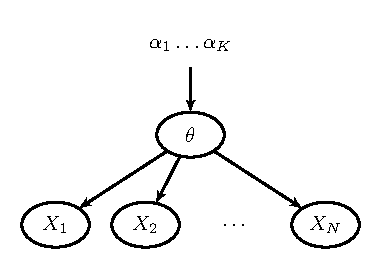
\includegraphics[height=4cm]{polya_bn.pdf}
\par\end{centering}
\caption{The Bayes-net for $N$ samples of a $K$-valued Categorical random variable.}
\label{fig:polya_bn}
\end{figure}

It follows directly from this Bayes net that their joint distribution
is given by:
\begin{align*}
  p(X_1\ldots X_N,\bm{\theta};\bm{\alpha})
  &= p(\bm{\theta};\bm{\alpha}) \prod_{n} p(X_n|\bm{\theta}).
\end{align*}

These Dirichlet-Categorical dependencies are known as
Dirichlet-multinomial (also the name of the WIKI page on this) or
Polya distributions. In a graphical model description we focus on the
individual $\bm{\theta},X_i$ interactions. There might also be further
random variables depending on these Categorical RVs. To develop our
understanding we briefly investigate the flow of information in the
simplified situation shown in Fig.~\ref{fig:polyabasic}.

\begin{figure}[!h]
  \begin{centering}
    \parbox{0.9\textwidth}{
      \centering
      \psfragfig[height=6cm,crop=pdfcrop,angle=-90]{polyabasic_bn}\\
      (a) Bayes net
    }\\[5mm]
  \end{centering}
  %%%%%%%%%%%%%%
  \begin{centering}
    \parbox{0.9\textwidth}{ \centering
      \psfragfig[height=10cm,crop=pdfcrop,angle=-90]{polyabasic_cg}\\ (b)
      Cluster graph: The center cluster is the Polya distribution,
      with the pure Dirichlet cluster to its left and a pure
      Categorical cluster to its right.}
  \end{centering}
  %%%%%%%%%%%%%%
  \caption{A simple Dirichlet-Polya graphical model to be used as a
    running example for factor operators. Parameters: $\alpha_0 =
    0.8$, $\alpha_1 = 1.2$ and $p(X=Y)=0.8$. We assume that $Y=1$ is
    observed.}  \label{fig:polyabasic}
\end{figure}

\section{The joint distribution}

The full joint is now given by $p(Y,X,\bm{\theta};\bm{\alpha}) =
p(Y|X)p(X|\bm{\theta})p(\bm{\theta};\bm{\alpha})$. Let us first focus on:
\begin{align}
  p(X,\bm{\theta};\bm{\alpha})
  &= p(X|\bm{\theta})p(\bm{\theta};\bm{\alpha}) \notag\\
  &= \frac{\Gamma(\sum_k \alpha_k)}{\prod_{k}\Gamma(\alpha_k)}
  \prod_{k}\theta_k^{\alpha_k-1} \prod_{k} \theta_k^{\mathbb{[}X=k\mathbb{]}} && \text{(combining Eqs.~\ref{eq:categorical} and
\ref{eq:dirichlet}) }\notag \\
  &= \frac{\Gamma(\sum_k \alpha_k)}{\prod_{k}\Gamma(\alpha_k)}
  \prod_{k}\theta_k^{\mathbb{[}X=k\mathbb{]}+\alpha_k-1}. \label{eq:polya}
\end{align}

Note that, for this joint Polya to exist, we first needed to multiply
in the Dirichlet prior $p(\bm{\theta};\bm{\alpha})$.

Assuming that $X$ and $\bm{\theta}$ both are unobserved, we will have
to marginalise $\bm{\theta}$ out of this joint to further propagate
information towards the $Y|X$ cluster. We then get:
\begin{align*}
p(X;\bm{\alpha}) &= \int_{\bm{\theta}} p(X,\bm{\theta};\bm{\alpha})d\bm{\theta} \\
p(Y,X;\bm{\alpha}) &= p(Y|X)p(X;\bm{\alpha}).
\end{align*}

Observing $Y = \mathsf{y}$ and then normalising over $X$ immediately
gives us a distribution $p(X|Y=\mathsf{y};\bm{\alpha})$.  Dividing
this by $p(X;\bm{\alpha})$ gives the message $p(X|Y=\mathsf{y})$ which
now needs to be multiplied in at the Polya cluster, enriching it with
the knowledge as to what value $Y$ was. We now have the marginal
$p(X,\bm{\theta}|Y = \mathsf{y};\bm{\alpha})$ at the Polya
cluster. Marginalising $X$ out from this, and then dividing by the
$p(\bm{\theta};\bm{\alpha})$ originally sent from the Dirichlet
cluster, gives the resultant message
\begin{align*}
  p(\bm{\theta}|Y =
\mathsf{y}) &= \frac{\sum_Xp(X,\bm{\theta}|Y =
\mathsf{y};\bm{\alpha})}{p(\bm{\theta};\bm{\alpha})}.
\end{align*}
to now send to the Dirichlet cluster. Finally, multiplying this with
the original $p(\bm{\theta};\bm{\alpha})$ gives the marginal
$p(\bm{\theta}|Y = \mathsf{y};\bm{\alpha})$. In the following sections
we provide more detail on these (and other) operations.

\section{Sampling}
This is pretty easy.
\begin{description}
  \item[Step 1:] You first sample the Dirichlet distribution as
    explained above to get values for $\bm{\theta}$. These are the
    respective (discrete) probabilities applicable to the Categorical
    variable $X$.
  \item[Step 2:] Simply sample $X$ accordingly to get the sample
    $(\bm{\mathsf{\theta}},\mathsf{x})$.
  \item [Question:] What about the case where the Polya also gets
    multiplied with an incoming $p(X)$ message? Answ: Should not be a
    problem, we sample only in the causal direction.
\end{description}

\section{Observing values} \label{sec:polya_obsv}

\subsubsection{Observing $\bm{\theta}$:}~\\
If we get to observe $\bm{\theta}$, we no longer have any need for a
Polya distribution. The $p(X|\bm{\theta})$ reduces to a standard
normalised Categorical distribution.

\subsubsection{Observing $X$:}~\\
If we observe that $X=\mathsf{x}$, the Polya distribution changes to a
pure Dirichlet form:
\begin{align}
  p(X=\mathsf{x}, \bm{\theta};\bm{\alpha})
  &\propto \frac{\Gamma(\sum_k\alpha_k) }{\prod_{k}\Gamma(\alpha_k)}
  \prod_{k}\theta_k^{\mathbb{[}\mathsf{x}=k\mathbb{]}+\alpha_k-1}. \label{eq:polya_obsvx}
\end{align}

Let us now determine the volume of this resultant distribution. By
inspecting the factors in the product we recognise the form of a
Dirichlet distribution with all the $\alpha_k$ values intact, apart
from the $\mathsf{x}$'th factor which has a new parameter value of
$\alpha'_{\mathsf{x}} = \alpha_{\mathsf{x}}+1$.

To determine the volume of the above we first we need a little
integration trick. Applying the fact that a probability distribution
must have unity volume to Eq~\ref{eq:dirichlet} gives:
\begin{align}
  \int_{\bm{\theta}}\frac{\Gamma(\sum_k\alpha_k)}{\prod_{k}\Gamma(\alpha_k)}
  \prod_{k}\theta_k^{\alpha_k-1} d\bm{\theta} &= 1 \notag\\
  \therefore \int_{\bm{\theta}} \prod_{k}\theta_k^{\alpha_k-1} d\bm{\theta}
  &= \frac{\prod_{k}\Gamma(\alpha_k)}{\Gamma(\sum_k\alpha_k)} \label{eq:dir_int_trick}
\end{align}

From this follows that:
\begin{align}
  \frac{\Gamma(\sum_j\alpha_j)}{\prod_{j}\Gamma(\alpha_j)} \int_{\bm{\theta}}
  \prod_{k}\theta_k^{\mathbb{[}\mathsf{x}=k\mathbb{]}+\alpha_k-1} d\bm{\theta}
  &= \frac{\Gamma(\sum_j{\alpha_j})}{\prod_{j}\Gamma(\alpha_j)} \frac{\Gamma(1+\alpha_\mathsf{x})\prod_{k\neq{\mathsf{x}}}\Gamma(\alpha_k)}{\Gamma(1+\sum_k\alpha_k)},\notag \\
  &= \frac{\Gamma(\sum_j{\alpha_j})}{\prod_{j}\Gamma(\alpha_j)} \frac{\alpha_\mathsf{x}\Gamma(\alpha_\mathsf{x})\prod_{k\neq{\mathsf{x}}}\Gamma(\alpha_k)}{\Gamma(\sum_k\alpha_k)\sum_k\alpha_k}, \notag \\
  &= \frac{\alpha_\mathsf{x}}{\sum_k\alpha_k}. \label{eq:polya_obsvx_vol}
\end{align}
We therefore know exactly what the volume is after we sliced through
the Polya at the observed value of $X$. This makes it easy to
renormalise by dividing by the quantity in Eq.~\ref{eq:polya_obsvx_vol}.

To find the message to send back to the original Dirichlet node, we
need to divide out the (incoming) message sent from the Dirichlet to
the Polya node. Working directly from the unnormalised distribution in
Eq.~\ref{eq:polya_obsvx} results in:

\begin{align}
  p(\bm{\theta}|X=\mathsf{x})
  &= \prod_{k}\theta_k^{\mathbb{[}\mathsf{x}=k\mathbb{]}}. \label{eq:polya_observed}
\end{align}
We recognise this as a properly normalised Dirichlet distribution with
$\alpha_{k\neq \mathsf{x}}=1$ and $\alpha_{\mathsf{x}}=2$.

This is a very satisfying result:
\begin{itemize}
  \item It matches the intuitive understanding that observing a single
    count of $X = \mathsf{x}$ should contribute a single count towards
    its Dirichlet phantom counts.
  \item We will also find this result useful as a sanity check when we
    are marginalising a Polya over $X$. Specifically, when a
    particular $X = \mathsf{x}$ has probability one (and the other
    values of $X$ therefore has a probability zero), is equivalent to
    observing $X = \mathsf{x}$. The resultant distributions should
    therefore also match.
  \item From a number of samples of $X$ this allows us to estimate the
    Dirichlet Distribution that those $X$'s arose from. Very useful
    for Monte-Carlo applications.
\end{itemize}

\section{Marginalising Eq.~\ref{eq:polya} over $\bm{\theta}$ (vanilla version)}
This one is fairly easy, and we will need its result in other places
too. So let us get it out of the way, reserving marginalising over $X$
for a later section.

Applying the integration trick of Eq.~\ref{eq:dir_int_trick} to
Eq.~\ref{eq:polya} while also remembering that $\Gamma(1+x) =
x\Gamma(x)$ yields:
\begin{align}
  p(X=\mathsf{x};\bm{\alpha})
  &= \int_{\bm{\theta}}p(X=\mathsf{x},\bm{\theta};\bm{\alpha})d\bm{\theta} \notag \\
  &= \frac{\Gamma(\sum_k\alpha_k))}{\prod_{k}\Gamma(\alpha_k)} \int_{\bm{\theta}} \prod_{k}\theta_k^{\mathbb{[}\mathsf{x}=k\mathbb{]}+\alpha_k-1}d\bm{\theta} \notag \\
  &= \frac{\Gamma(\sum_k\alpha_k))}{\prod_{k}\Gamma(\alpha_k)} \frac{\Gamma(1+\alpha_{\mathsf{x}})\prod_{k\neq\mathsf{x}}\Gamma(\alpha_k)}{\Gamma(1+\sum_k\alpha_k)} \notag\\
  &= \frac{\Gamma(\sum_k\alpha_k))}{\prod_{k}\Gamma(\alpha_k)} \frac{\alpha_{\mathsf{x}}\Gamma(\alpha_{\mathsf{x}})\prod_{k\neq\mathsf{x}}\Gamma(\alpha_k)}{\sum_k(\alpha_k)\Gamma(\sum_k\alpha_k)} \notag\\
  &=  \frac{\alpha_{\mathsf{x}}}{\sum_k\alpha_k}. \label{eq:marg_theta_van}
\end{align}

\section{Multiplication} \label{sec:polya_mpy}
\subsubsection{Multiplication (from the left) with $p(\bm{\theta};\bm{\alpha})$:}~\\
We have pretty much covered this one already, this is how we formed
the Polya joint in the first place. The result is given in
Eq.~\ref{eq:polya}.

\subsubsection{Multiplication (from the right) with $p(X|Y=\mathsf{y})$:}~\\
To simplify things we are doing the following with $X$ a binary
variable. The results, however, straightforwardly carry over to the
more general case of Categorical variables.

Let us rewrite Eq.~\ref{eq:polya} into a form that makes the role of
$X$ more explicit:
\begin{align*}
  p(X,\bm{\theta};\bm{\alpha}) &= \left\{
    \begin{array}{lr}
    c\theta_0^{\alpha_0}\theta_1^{\alpha_1-1} & \mbox{ with } X=0\\
    c\theta_0^{\alpha_0-1}\theta_1^{\alpha_1} & \mbox{ with } X=1
\end{array}
\right.,
\end{align*}
with
\begin{align*}
  c &= \frac{\Gamma(\alpha_0+\alpha_1)}{\Gamma(\alpha_0)\Gamma(\alpha_1)}.
\end{align*}

I.e. the joint density consists of two separate/distinct (continuous)
Dirichlet functions with a combined unity volume. We can determine
their respective volumes via Eq.~\ref{eq:marg_theta_van} as:
\begin{align*}
  p(X=\mathsf{0};\bm{\alpha}) &= \frac{\alpha_0}{\alpha_0+\alpha_1} & \text{and}\\
  p(X=\mathsf{1};\bm{\alpha}) &= \frac{\alpha_1}{\alpha_0+\alpha_1}.
\end{align*}

Multiplying the joint with
\begin{align*}
  p(X|Y=\mathsf{y}) &= \left\{
    \begin{array}{lr}
    p_0 & \mbox{ with } X=0\\
    p_1 & \mbox{ with } X=1
\end{array}
\right.
\end{align*}
results in:

\begin{align*}
  p(X,\bm{\theta};\bm{\alpha})p(X|Y=\mathsf{y}) &= \left\{
  \begin{array}{lr}
    p_0c\theta_0^{\alpha_0}\theta_1^{\alpha_1-1} & \mbox{ with } X=0\\
    p_1c\theta_0^{\alpha_0-1}\theta_1^{\alpha_1} & \mbox{ with } X=1
  \end{array}
  \right..
\end{align*}

The two volumes rescale with $p_0$ and $p_1$ respectively so that
their non-normalised relative volumes become:
\begin{align*}
  p(X=\mathsf{0}|Y=\mathsf{y};\bm{\alpha}) &= \frac{p_0\alpha_0}{\alpha_0+\alpha_1} & \text{and}\\
  p(X=\mathsf{1}|Y=\mathsf{y};\bm{\alpha}) &= \frac{p_1\alpha_1}{\alpha_0+\alpha_1}.
\end{align*}

This product therefore has an unnormalised volume of:
\begin{align*}
  d &= \frac{p_0\alpha_0 + p_1\alpha_1}{\alpha_0+\alpha_1} \leq 1.
\end{align*}

Finally our normalised joint distribution becomes:

\begin{align}
  p(X,\bm{\theta};\bm{\alpha})p(X|Y=\mathsf{y}) &= \left\{
  \begin{array}{lr}
    \frac{p_0c}{d}\theta_0^{\alpha_0}\theta_1^{\alpha_1-1} & \mbox{ with } X=0\\
    \frac{p_1c}{d}\theta_0^{\alpha_0-1}\theta_1^{\alpha_1} & \mbox{ with } X=1
  \end{array}
  \right.. \label{eq:polya_updated}
\end{align}

\textbf{Note:} It is tempting to replace this product with a new Polya
with parameters $\alpha_i^{'} = p_i\alpha_i$. It is easy to see that
this is wrong.

\section{Marginalising Eq.~\ref{eq:polya_updated} over $\bm{\theta}$ (stracciatella version)}
When using the belief update (BU) algorithm (in general), or even
using the belief propagation (BP) algorithm in a more complex
situation (where multiple Categorical distributions are linked to the
Polya -- see for instance $p(X_3|\bm{\theta})$ in
Fig.~\ref{fig:polya_example}) transforms the Polya joint to the
situation depicted in Eq.~\ref{eq:polya_updated}. If we now
marginalise over $\bm{\theta}$ to find the probability of
$X=\mathsf{x}$:
\begin{align}
  p(X=\mathsf{x};\bm{\alpha},\ldots)
  &= \int_{\bm{\theta}} p(X=\mathsf{x},\bm{\theta};\bm{\alpha})p(X=\mathsf{x}|Y=\mathsf{y})d\bm{\theta}
  && \text{(marginalising Eq.~\ref{eq:polya_updated})} \notag\\
  &= \frac{p_\mathsf{x}c}{d}\int_{\bm{\theta}}\prod_i \theta_i^{[i=\mathsf{x}]+\alpha_i-1} d\bm{\theta} \notag\\
  &= \frac{p_\mathsf{x}}{d}\frac{\Gamma(\sum_i\alpha_i)}{\prod_i\Gamma(\alpha_i)}
  \frac{\prod_i\Gamma([i=\mathsf{x}] + \alpha_i)}{\Gamma(1+\sum_i\alpha_i)}
  && \text{(using Eq.~\ref{eq:dir_int_trick})}\notag\\
  &= \frac{p_\mathsf{x}\sum_i\alpha_i}{\sum_ip_i\alpha_i}\frac{\Gamma(\sum_i\alpha_i)}{\prod_i\Gamma(\alpha_i)}
  \frac{\alpha_\mathsf{x}}{\sum_i\alpha_i}\frac{\prod_i\Gamma(\alpha_i)}{\Gamma(\sum_i\alpha_i)}
  && (\text{with } d = \frac{\sum_ip_i\alpha_i}{\sum_i\alpha_i})\notag\\
     &= \frac{p_\mathsf{x}\alpha_\mathsf{x}}{\sum_ip_i\alpha_i} \label{eq:marg_theta_strac}.
\end{align}

Note that the denominator is independent of $\mathsf{x}$ -- it simply
serves as a normalisation term. The probability that $X=\mathsf{x}$ is
proportional to $p_\mathsf{x}\alpha_\mathsf{x}$.

\section{Marginalising Eq.~\ref{eq:polya} over $X$ (vanilla version)}
To make things more explicit, let us consider Eq.~\ref{eq:polya} for the binary case:
\begin{align*}
  p(X,\bm{\theta};\bm{\alpha}) &= \frac{\Gamma(\sum_i\alpha_i)}{\prod_i\Gamma(\alpha_i)}\left\{
    \begin{array}{lr}
    \theta_0^{\alpha_0}\theta_1^{\alpha_1-1} & \mbox{ with } X=0\\
    \theta_0^{\alpha_0-1}\theta_1^{\alpha_1} & \mbox{ with } X=1
\end{array}
\right..
\end{align*}
Marginalising this over $X$ gives:
\begin{align}
  p(\bm{\theta};\bm{\alpha})
  &= \frac{\Gamma(\sum_i\alpha_i)}{\prod_i\Gamma(\alpha_i)}
  \left(\theta_0\theta_0^{\alpha_0-1}\theta_1^{\alpha_1-1} + \theta_1\theta_0^{\alpha_0-1}\theta_1^{\alpha_1-1}\right) \notag\\
  &= \frac{\Gamma(\sum_i\alpha_i)}{\prod_i\Gamma(\alpha_i)}
  \theta_0^{\alpha_0-1}\theta_1^{\alpha_1-1}
  \left(\theta_0+\theta_1\right) \notag\\
  &= \frac{\Gamma(\sum_i\alpha_i)}{\prod_i\Gamma(\alpha_i)}
  \theta_0^{\alpha_0-1}\theta_1^{\alpha_1-1} && \text{(the $\theta$'s sum to one)}.
\end{align}
This should not come as a huge surprise. If no other information
entered the system, we get our original Dirichlet back. In the next
section we consider the case where an incoming message over $X$ alters
our knowledge of the situation.

As an aside, note that marginalising Eq.~\ref{eq:polya_updated} while
limiting $p(X|Y=\mathsf{y})$ to be flat/uniform, would have yielded
the same result.

\section{Marginalising Eq.~\ref{eq:polya_updated} over $X$ (stracciatella version)}

We now turn our attention to the message/distribution that must be
passed back from the Polya cluster to the Dirichlet cluster assuming
that we have received a message from the $X|Y$ cluster. To marginalise
we once again sum over the values of $X$:

\begin{align}
  p(\bm{\theta}|Y=\mathsf{y};\bm{\alpha})
  &= \sum_{\mathsf{x}} p(X,\bm{\theta}|Y=\mathsf{y};\bm{\alpha}) \notag \\
  &= \frac{p_0c}{d}\theta_0^{\alpha_0}\theta_1^{\alpha_1-1} + \frac{p_1c}{d}\theta_0^{\alpha_0-1}\theta_1^{\alpha_1} \notag\\
  &= c\theta_0^{\alpha_0-1}\theta_1^{\alpha_1-1}\frac{\left[p_0\theta_0+p_1\theta_1 \right]}{d}, \text{ or in general}\notag\\
  &= \left(c\prod_k\theta_k^{\alpha_k-1}\right)\left(\frac{\sum_kp_k\theta_k}{d}\right). \label{eq:dirich_true_post}
\end{align}

We recognise this as the message originally received from the
Dirichlet cluster, multiplied by a (flat) hyperplane over
$\bm{\theta}$. Note that, with all $p_k$ values equal, this will once
again revert to the result obtained in the previous section (i.e. we
simply return the original Dirichlet).

Note that, since we marginalised the full joint, we still have to
divide out the original Dirichlet message before assimilating the
result in the Dirichlet prior. This leaves us with a hyperplane over
the $\theta$-space parameterised by the various $p_k$ values to pass
on to the Dirichlet cluster. Intuitively satisfying, this message
travelling from the right to the left in Fig.~\ref{fig:polyabasic}
does not depend on the $\alpha_k$ values.

\subsection{How to approximate the marginal}
Unfortunately Eq.~\ref{eq:dirich_true_post} is not in a form conjugate
to the Dirichlet parameterisation and we will have to approximate it
with something more suitable.  We can approach this approximation
either from an optimisation angle, or from a sampling angle.

\begin{enumerate}
\item Using optimisation we can minimise the Kullback-Leibler divergence
  between Eq.~\ref{eq:dirich_true_post} and its Dirichlet
  approximation. Depending on the order of the two distributions this
  leads to either:
  \begin{enumerate}
  \item Forward / moment approximation: expectation propagation (EP)
    or
  \item reversed / information approximation: variational message
    passing (VMP).
  \end{enumerate}
  We will return to these topics later.
\item Instead we use a sampling approach in the following. The reasoning is as
  follows:
  \begin{enumerate}
  \item We know how to update the Dirichlet posterior if we observe
    values for $X$. We simply increment the count of the
    corresponding $\alpha$ values.
  \item The given model is sufficiently detailed that we can sample a
    large number of $X$ values from it. We can use these samples to
    update the Dirichlet correspondingly.
  \item By carefully paying attention to the relative proportions of
    $X$ values, we can infer the general formula that should be
    applicable with infinitely many samples.  This should be the
    marginalisation we are looking for.
  \end{enumerate}
\end{enumerate}

In the next section we apply this sampling approach and find,
surprisingly, that the approximation also depends on the $\alpha_k$
values.

\subsection{Marginalisation via hierarchical sampling}

Our first approach is to do a large number of simulations of the
situation depicted in Fig.~\ref{fig:polyabasic}. From these we can
remove all cases where $Y$ does not match the observation
$Y=\mathsf{y}$ we made. The remaining cases depict sampled values of
$X$ consistent with both the model structure and the observed $Y$
values. We can then combine the averaged occurrences of the
corresponding $X$ values with the original Dirichlet priors in an
estimate of the Dirichlet posterior. From this we can deduce what the
message passed from the Polya cluster to the Dirichlet cluster, should
be. Let's dive into the detail:

In Figure~\ref{fig:polyabasic} we encounter three different
distribution clusters, each conditionally dependent on the one coming
before it. Let's summarise each of them:

First we sample $\bm{\theta}$ from the Dirichlet distribution given by:
\begin{align*}
  p(\bm{\theta};\bm{\alpha}) &\propto \theta_0^{\alpha_0-1}\theta_1^{\alpha_1-1}.
\end{align*}

If we stick this $\bm{\mathsf{\theta}}$ into the Polya distribution,
it changes to a Categorical distribution in $X$ given by:
\begin{align*}
  p(X|\bm{\theta}) &= \left\{
    \begin{array}{lr}
    \mathsf{\theta_0} & \mbox{ with } X=0\\
    \mathsf{\theta_1} & \mbox{ with } X=1\\
    \end{array}
    \right..
\end{align*}

We sample $X=\mathsf{x}$ from it and stick it into the distribution
for $p(Y|X)$:\\
%\begin{table}[!h]
    \begin{center}
    \begin{tabular}{c c|l}
    $X$ & $Y$ & $p(Y|X)$\\ \hline
    0 & 0 & 0.8 \\
    0 & 1 & 0.2 \\
    1 & 0 & 0.2 \\
    1 & 1 & 0.8
    %\multicolumn{2}{c|}{elsewhere} & 0.0 \\
    \end{tabular}
    \end{center}
 % \caption{Probability factor $p(Y|X)$. }
%\end{table}

This gives us a distribution over $Y$ as dictated by the particular
$\mathsf{x}$ (it picks out either the top or bottom half of this
table). We then sample $Y$ from this distribution.  From the
description from Fig.~\ref{fig:polyabasic} we know that the observed
value of $Y$ should be 1. If this matches our sample, we record this
specific run of samples. If not, we discard it and start anew. For each
one of the retained sample runs, we can estimate a posterior Dirichlet
by updating its $\alpha$ parameters to:
\begin{align*}
  \alpha'_k &= \alpha_k+[x=k]
\end{align*}

After having completed many sampling runs, we can simply average each
set of $\alpha_k$ values over the runs thereby estimating the
posterior value for $\alpha_k$. Table~\ref{tab:samplepolya} gives the results for such
a simulation over 100k accepted runs:
\begin{table}[!h]
\begin{center}
  \begin{tabular}{c | cc}
    $k$ & 0 & 1\\ \hline
    $\alpha_k$ & 0.8 & 1.2 \\
    $\sum_n[x_n=k]$ & 14247 & 85753 \\
    $\frac{1}{100000}\sum_n \alpha_k + [x_n=k]$ & 0.94247 & 2.05753
  \end{tabular}
\end{center}
\caption{Estimating posterior $\bm{\alpha}$ via hierarchical sampling from Fig.~\ref{fig:polyabasic}.  \label{tab:samplepolya} }
\end{table}

Let's analytically confirm this:
\begin{align*}
  p(X,Y,\bm{\theta};\bm{\alpha}) &= p(Y|X)p(X|\bm{\theta})p(\bm{\theta};\bm{\alpha})\\
  \therefore p(X,Y;\bm{\alpha}) &= p(Y|X)\int_{\bm{\theta}} p(X,\bm{\theta};\bm{\alpha}) d\bm{\theta} \\
  \therefore p(X=\mathsf{x},Y;\bm{\alpha}) &= p(Y|X=\mathsf{x})\frac{\alpha_{\mathsf{x}}}{\sum_k{\alpha_k}}.
\end{align*}
If we now observe $\mathsf{y}$ this reduces to:
\begin{align*}
  p(X=\mathsf{x},Y=\mathsf{y};\bm{\alpha}) &= p(Y=\mathsf{y}|X=\mathsf{x})\frac{\alpha_{\mathsf{x}}}{\sum_k{\alpha_k}} \\
  &= \frac{p_{\mathsf{x}}\alpha_{\mathsf{x}}}{\sum_k{\alpha_k}},
\end{align*}
where $\mathsf{y}$ is the observed value of $Y$ and $p_{\mathsf{x}} =
p(Y=\mathsf{y}|X=\mathsf{x})$. To determine
$p(X=\mathsf{x}|Y=\mathsf{y};\bm{\alpha})$ we simply normalise this
function over all the possible values of $\mathsf{x}$. This reduces the expression to
\begin{align}
  p(X=\mathsf{x}|Y=\mathsf{y};\bm{\alpha}) &= \frac{p_{\mathsf{x}}\alpha_{\mathsf{x}}}{\sum_k{p_k\alpha_k}}.
  \label{eq:dirich_est_msg}
\end{align}
This gives the fraction of times we will expect to see $X =
\mathsf{x}$. To get our posterior Dirichlet estimate $\bm{\alpha}'$ we still
need to add the original $\bm{\alpha}$ values to this:
\begin{align}
  \alpha'_{\mathsf{x}} &= \frac{p_{\mathsf{x}}\alpha_{\mathsf{x}}}{\sum_k{p_k\alpha_k}} + \alpha_{\mathsf{x}}.
  \label{eq:dirich_est_post}
\end{align}
From this equation we confirm that $p_{\mathsf{x}}=1$ simply adds one
to the corresponding original $\alpha_{\mathsf{x}}$ (as expected).
Applying this to Fig.~\ref{fig:polyabasic} with $y=1$ yields
$\alpha'_0 = 0.94286, \alpha'_1= 2.05714$.  This beautifully matches
our previous experimentally obtained values. We have our first
approximate Polya marginalisation over $X$. And, surprisingly, it is
dependent on the $\alpha$ values originally supplied by the
destination Dirichlet distribution!

TODO: Add reasoning on how to move from this posterior to the required
marginalisation of the Polya. (Answ: same expression)

\begin{figure}[!h]
  \begin{centering}
    \parbox{0.48\textwidth}{
      \centering
      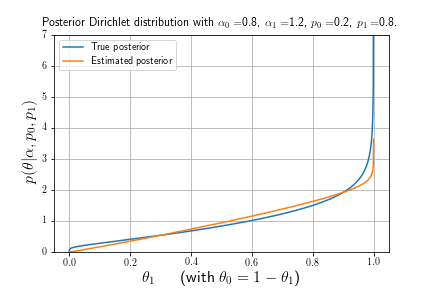
\includegraphics[width=0.48\textwidth]{pdir1.png}
      (a) The parameter set from Fig.~\ref{fig:polyabasic} approximates well.
    }
  \end{centering}
  %%%%%%%%%%%%%%
  \begin{centering}
    \parbox{0.48\textwidth}{ \centering
      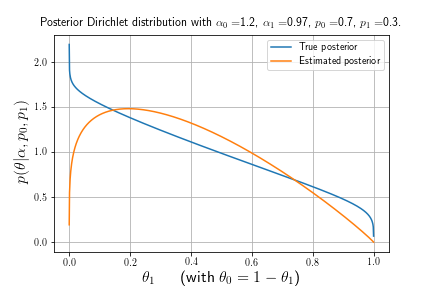
\includegraphics[width=0.48\textwidth]{pdir2.png}
      (b) This parameter set seems to be more difficult to approximate.
    }
  \end{centering}
  %%%%%%%%%%%%%%
  \caption{Comparing the true Dirichlet posterior as in
    Eq.~\ref{eq:dirich_true_post} to its approximation via
    Eq.~\ref{eq:dirich_est_post}. Clearly the quality of the
  approximation varies from case to case.}
\label{fig:post_dirichlet}
\end{figure}

\subsection{Say whattt?}
\subsection{Recap}
With reference to Fig.~\ref{fig:polyabasic}(b) we noticed that the
true posterior given by Eq.~\ref{eq:dirich_true_post}:
\begin{align}
  p(\bm{\theta}|Y=\mathsf{y};\bm{\alpha})
  &= \left(c\prod_k\theta_k^{\alpha_k-1}\right)\left(\frac{\sum_kp_k\theta_k}{d}\right), \nonumber
\end{align}
is not conjugate to the Dirichlet prior. The message that we ideally
want to send from the Polya cluster to the Dirichlet, after cancelling
the incoming message to the Polya, would have been the hyperplane
$\frac{\sum_kp_k\theta_k}{d}$, but this also is not conjugate to the
Dirichlet. We need to somehow approximate this with a message that
\emph{is} conjugate. To solve this we make use a thought experiment
where we imagine a large number of samples of the random variables
involved. In such a fully sampled situation each sample set allocates
values to all the variables, therefore replacing all latent variables
with observed samples. From these samples we can do a ML/MAP estimate
of the parameters of the posterior Dirichlet distribution - we do this
by averaging the appropriate estimate from each of these samples.

However, this sampling and averaging is a laborious business. If we
really wanted to go this way, we would have used an MCMC procedure in
the first place. Can we achieve the same result without actually doing
the sampling? The answer turns out to be yes. For each observation
$X=k$, we know that the ML estimate simply adds a single count to the
corresponding $\alpha_k$ parameter. We are averaging out over all the
observations, we therefore need to divide each of these counts with
the number of samples. So in effect ultimately each $\alpha_k$ is
incremented with $p(X=k|\text{everything else})$. But we can actually
calculate these probabilities directly, this is exactly what is given
in Eq.~\ref{eq:dirich_est_msg}! QED.

\subsection{Yeah right, but what exactly is actually going down here?}
The explanation here still needs to be properly verified. But this is
what I think is going on.

\subsubsection{The Dirichlet distribution as a member of the Exponential Family}

We can rewrite Eq.~\ref{eq:dirichlet} into exponential form by setting
\begin{align}
  h(\bm{x})      &= 1, \\
  \bm{\eta}      &= \left[\alpha_0-1, \alpha_1-1, \hdots, \alpha_{K-1}-1\right]^T, \\
  Z(\bm{\eta})   &= \frac{\prod_k\Gamma(\alpha_k)}{\Gamma(\sum_k \alpha_k)} \text{ and } \\
  \bm{T}(\bm{x}) &= \left[\log \theta_0, \log \theta_1, \hdots, \log \theta_{K-1}\right]^T.
\end{align}

We can find the parameters by noting the relationship:
\begin{align}
  \nabla_{\bm{\eta}} Z(\bm{\eta})
  &= \mathbb{E}\left[\bm{T}(\bm{x})\right] \label{eq:dlogZ} \\
  &= \frac{1}{N}\sum_n\bm{T}(\bm{x}_n) \label{eq:momentmatch}.
\end{align}

Unfortunately these do not have closed form solutions and must be solved iteratively. For the Dirichlet distribution
Eq.~\ref{eq:dlogZ} reduces to:
\begin{align}
  \Psi(\alpha_k) - \Psi(\sum_k\alpha_k) &= \log \theta_k.
\end{align}

Somehow Eq.~\ref{eq:dirich_est_post} ends up being a decent approximation to this.


\subsection{Variational marginalisation}
Eq~\ref{eq:dirich_true_post} gives the true posterior for
$\bm{\theta}$ as:
\begin{align}
  p(\bm{\theta}|Y=y;\bm{\alpha})  &= c\prod_k\theta_k^{\alpha_k-1}\frac{\sum_kp_k\theta_k}{d}.
\end{align}
We could also have approached this directly as a variational
problem. The message passing aspects are the same, but the
minimisation can now be considered explicitly. The resulting
approximate distribution must have the following (conjugate) form:
\begin{align}
  q(\bm{\theta};\bm{\beta})  &= \frac{\sum_k\beta_k}{\prod_k\Gamma(\beta_k)}\prod_{k}\theta_k^{\beta_k-1}.
\end{align}
We can optimise the approximation by minimising the KL divergence in
one of two directions:

\paragraph{Approximation via variational inference}
Minimise
\begin{align*}
  \text{KL}[q(\bm{\theta};\bm{\beta})||p(\bm{\theta}|Y=y;\bm{\alpha})]
  &= \int_{\bm{\theta}} q(\bm{\theta};\bm{\beta})
  \log{\frac{q(\bm{\theta};\bm{\beta})}{p(\bm{\theta}|Y=y;\bm{\alpha})} d\bm{\theta}} \\
  &= \int_{\bm{\theta}}
  \frac{\Gamma(\sum_k\beta_k)}{\prod_k\Gamma(\beta_k)}\prod_{k}\theta_k^{\beta_k-1}
  \log \left[
    \frac{\frac{\Gamma(\sum_k\beta_k)}{\prod_k\Gamma(\beta_k)}\prod_{k}\theta_k^{\beta_k-1}}
         {c\prod_k\theta_k^{\alpha_k-1}\frac{\sum_kp_k\theta_k}{d}}
         \right] d\bm{\theta},
\end{align*}
w.r.t. $\bm{\beta}$. TOBECOMPLETED

\paragraph{Approximation via expectation propagation}
Minimise
\begin{align*}
  \text{KL}[p(\bm{\theta}|Y=y;\bm{\alpha})||q(\bm{\theta};\bm{\beta})]
  &= \int_{\bm{\theta}} p(\bm{\theta}|Y=y;\bm{\alpha})
  \log{\frac{p(\bm{\theta}|Y=y;\bm{\alpha})}{q(\bm{\theta};\bm{\beta})} d\bm{\theta}} \\
  &= \int_{\bm{\theta}}
  c\prod_k\theta_k^{\alpha_k-1}\frac{\sum_kp_k\theta_k}{d}
  \log \left[
    \frac{c\prod_k\theta_k^{\alpha_k-1}\frac{\sum_kp_k\theta_k}{d}}
         {\frac{\Gamma(\sum_k\beta_k)}{\prod_k\Gamma(\beta_k)}\prod_{k}\theta_k^{\beta_k-1}}
         \right] d\bm{\theta},
\end{align*}
w.r.t. $\bm{\beta}$. TOBECOMPLETED

\section{Normalisation}
There are two operations that can disrupt the unitary volume of a
Polya distribution namely to observe one of its random variables, or
to multiply it with a distribution over one of its random variables.
Sections~\ref{sec:polya_obsv} and \ref{sec:polya_mpy} explicitly
quantifies this. We can therefore easily renormalise the distribution
whenever we have a need for that.

\section{Message smoothing / damping / distances}
This operator applies to the messages entering the Polya node. These
are either a Dirichlet or a Categorical. Since both of them are
already covered elsewhere, we can simply ignore this operator.

\section{Examples}

\subsubsection{Example:}
Fig.~\ref{fig:polya_example} shows an (contrived) example of the typical
use of a Polya in a cluster graph. In this example we do not get
to observe any of the $X_m \in \{0,1\},\hspace{2mm} m = 1\ldots 4$
directly, but can access their sums via $Y_{mn} = X_m+X_n$.

\begin{figure}[htb]
\noindent \begin{centering}
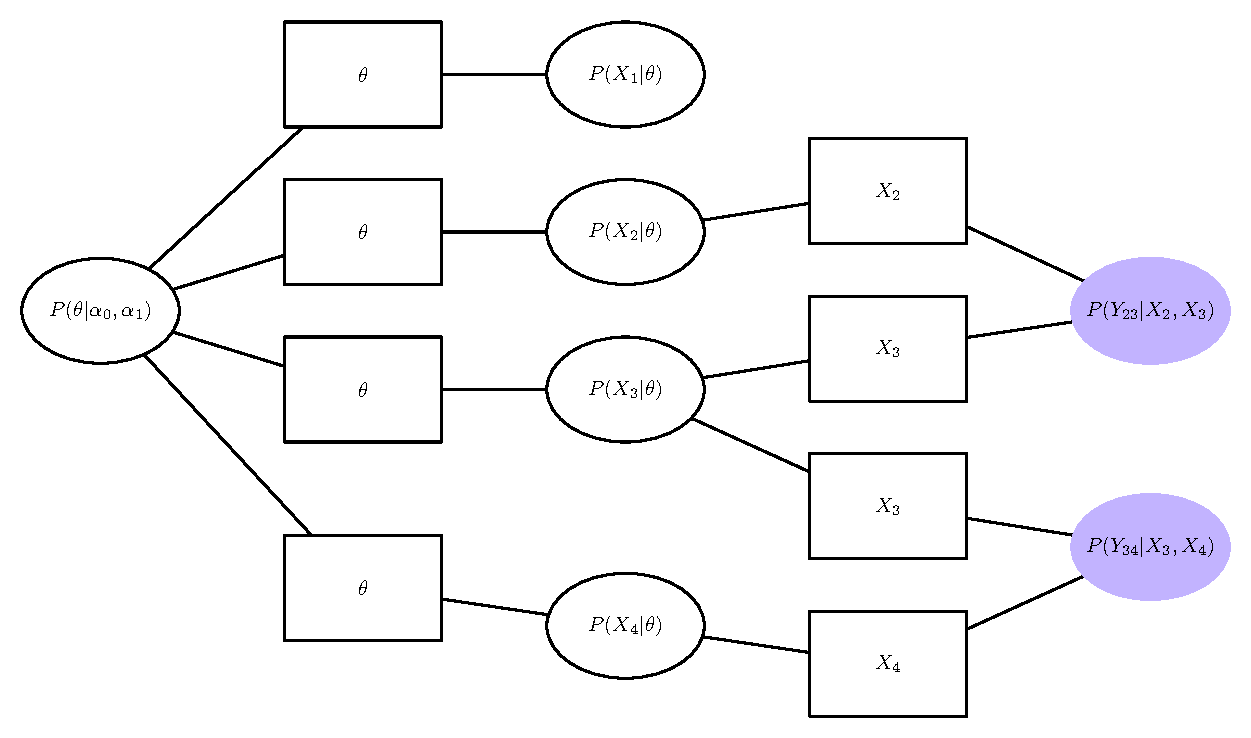
\includegraphics[height=8cm]{polya_example.pdf}
\par\end{centering}
\caption{Some coins $X_m \in \{0,1\},\hspace{2mm} m = 1\ldots 4$ are
  tossed, but sometimes we can only observe them indirectly via the
  $Y_{mn}$ variables. With $Y_{mn} = X_m+X_n$ with $Y_{mn} \in \{0,1,2\}$. Determine
$p(\theta| Y_{23}=0, Y_{34}=1;\alpha_0, \alpha_1)$? (Answ:
$\mbox{DIR}(\theta;\bm{\gamma})$ with $\gamma_0 =
\alpha_0+2$, $\gamma_1=\alpha_1+1$.)}
\label{fig:polya_example}
\end{figure}

\part{Conditional Categoricals and Company}

\chapter*{Some examples of conditional categoricals}

\section*{Bayesian inference of the parameters in a Hamming (7,4) error code}

Fig.~\ref{fig:hamming74a_bn} is the graphical model for the Hamming
(7,4) error correction code. Bits $b_0 \ldots b_3$ are the original
four (uncoded) bits to be sent. To that was added check bits $c_4,c_5$
and $c_6$ that added extra information dependent on the original four
(in this case enforcing even parity, but lets ignore that knowledge
for the moment). Now suppose we did not know the probabilities
$p(r_i|\text{pa}(r_i))$ and $p(c_i|\text{pa}(c_i))$. To find them we
either have to do some ML type of estimation, or handle the whole
situation using Bayesian inference. We are now going to investigate
this latter case.

\begin{figure}[htb]
  \begin{centering}
    \psfragfig[width=0.75\textwidth,crop=pdfcrop,angle=0]{hamming74a_bn}\\
    \caption{Bayes net for Hamming (7,4) code. The received bits
      $r_0\ldots r_6$ are observed.\label{fig:hamming74a_bn} }
  \end{centering}
\end{figure}

Note that each $\text{pa}(r_i)$ is a single $b_i$, where-as each
$\text{pa}(c_i)$ consists of several $b_i$'s. Both of these cases
represent conditional categoricals, but the multiplicity of marginals
implied by the latter case is going to be inconvenient. Following the
cue of Section~\ref{sec:multicat} we instead avoid the issue by
replacing these several parent nodes by a single parent which in its
turn is mapped to those multiple original parents. These newly
introduced 'mapped' latent variables appear as the various $z$
variables in Fig.~\ref{fig:hamming74b_bn}. The clustergraph in
Fig.~\ref{fig:hamming74b_cg} is useful to appreciate the various
marginalisations we defer to the purely categorical conditionals in
this manner.

Fig.~\ref{fig:hamming74b_bn} is the Bayesian version of
Fig.~\ref{fig:hamming74a_bn}. $\bm{\Theta}$ is a ConditionalDirichlet
prior describing the bit errors. Such a ConditionalDirichlet consists
of several Dirichlet distributions, one for each of the values that
the conditional variable can take on. Since we are assuming that all
bit errors have the same occurence probabilities, we have only a
single ConditionalDirichlet to describe this. In contrast, at the
bottom of the figure we allowed the parity check variables (the $z$'s)
to each have its own parity check logic - these are being described by
$\bm{\Phi}_{4\ldots 6}$.

We should be able to learn the distributions of all these Dirichlets
from observing enough packets $N$ of received bits $r_0 \ldots
r_6$. As an interesting aside one can also investigate how far one can
get with inferring the structure of the error coding if we initially
allow all the check bits to depend on all four message bits (instead
of just three). If we are able to learn which message bits
\emph{really} matter, we have also accomplished a type of structure
learning.

\begin{figure}[htb]
  \begin{centering}
    \psfragfig[width=0.75\textwidth,crop=pdfcrop,angle=0]{hamming74b_bn}\\
    \caption{Bayes net for Hamming (7,4) code with Bayesian
      priors. The received bits $r_0\ldots r_6$ are observed. Note the
      difference between the ConditionalPolyas at the $c_i$ nodes vs
      those at the $r_i$ nodes. In the case of the former the linked
      $r_i$ node creates an additional external distribution over the
      target $c_i$ node. In the case of the latter the $r_i$ nodes has
      no such external influence (recognisable by being linked only to
      its ConditionalDirichlet and conditioned-on nodes - i.e. only
      two connections). \\ Also note that $\bm{\Phi}_4, \bm{\Phi}_5
      \text{ and } \bm{\Phi}_6$ are three distinct
      ConditionalDirichlets, each consisting of eight internal
      Dirichlets (if we wanted to make use of the prior knowledge that
      they in fact only have one distribution, we also could have
      consolidated them into a single ConditionalDirichlet, also with
      eight internal Dirichlets). $\bm{\Theta}$ is just a single
      ConditionalDirichlet describing the errors in the received
      bits. \label{fig:hamming74b_bn} }
  \end{centering}
\end{figure}

\begin{figure}[htb]
  \begin{centering}
    \psfragfig[width=0.98\textwidth,crop=pdfcrop,angle=0]{hamming74b_cg}\\
    \caption{Cluster graph for Hamming (7,4) code with Bayesian
      priors.\label{fig:hamming74b_cg} }
  \end{centering}
\end{figure}

\FloatBarrier

\section*{Topic modelling via Latent Dirichlet Allocation (LDA)}

Fig.~\ref{fig:lda_bn} gives the structure used in topic modelling
(LDA) systems -- the $n$'th word in document $m$ is $W_{m,n}$. It
depends on the (latent) topic $Z_{m,n}$ present in the document, which
in its turn determines the appropriate Dirichlet RV
$\bm{\phi}_{\mathsf{z}_{i,j}}$ describing the words present in each
topic. (TO BE COMPLETED)

\begin{figure}[!h]
  \begin{centering}
    \parbox{0.95\textwidth}{
      \centering
      \psfragfig[width=0.9\textwidth,crop=pdfcrop,angle=0]{lda_bn}\\
      (a) Bayes net
    }\\[5mm]
  \end{centering}
  %%%%%%%%%%%%%%
  \begin{centering}
    \parbox{0.95\textwidth}{ \centering
      \psfragfig[width=0.2\textwidth,height=15cm,crop=pdfcrop,angle=-90]{lda_cg}\\ (b)
      Cluster graph}
  \end{centering}
  %%%%%%%%%%%%%%
  \caption{A Bayesian LDA system. The received bits $r_0\ldots r_6$
    are observed. $p(\bm{\theta}_m)$ is the Dirichlet distribution
    over the topics in document $m$. On the far right the Conditional
    Dirichlet $p(\bm{\Phi};\bm{B})$ contains the $K$ Dirichlet
    distributions $p(\bm{\phi}_k;\bm{\beta}_k)$ -- respectively
    describing the words in topic $k$. Also note the Conditional Polya
    distribution $p(W_{m,n}|Z_{m,n},\bm{\Phi})$, with latent $Z_{m,n}$
    selecting which of the $\bm{\phi}_k$'s to apply. The word
    $W_{m,n}$ is observed. \label{fig:lda_bn} }
\end{figure}


\chapter{Conditional Dirichlet}

\begin{figure}[!b]
  %%%%%%%%%%%%%%
  \begin{centering}
    \parbox{0.95\textwidth}{ \centering
      \psfragfig[width=0.5\textwidth,crop=pdfcrop,angle=0]{condpolya_bn}\\
      (a) Bayes net.}\\[5mm]
  \end{centering}
  %%%%%%%%%%%%%%
  \begin{centering}
    \parbox{0.95\textwidth}{ \centering
      \psfragfig[width=0.95\textwidth,crop=pdfcrop,angle=0]{condpolya_cg}\\
      (b) Cluster graph.}\\[5mm]
  \end{centering}
  %%%%%%%%%%%%%%
  \caption{Configuration to be used as a running example for
    conditional Polya operations. The latent RV $Z$ determines which
    $\bm{\phi}_{\mathsf{z}}$ to use to describe the probabilities of
    $Y$. We also included an RV $X$ to allow for other variables that
    also impacts on $Y$. $\bm{\beta}_k = [\beta_{k,0},\beta_{k,1},
      \ldots, \beta_{k,M-1}]^T$ is the vector of $\beta$ values
    applicable when $Z=k$ (with $M$ the cardinality of
    $Y)$. $\bm{\Phi};\bm{B}$ collects all the Dirichlets into one
    ConditionalDirichlet.\label{fig:condpolya} }
\end{figure}

We often have a situation where a categorical RV $Y$ (cardinality $M$)
is dependent on another categorical RV $Z$ (cardinality $K$). For any
given/known value of $Z$ the situation is exactly as we previously
encountered for Dirichlet and Polya distributions. However, with $Z$
latent, we now need $K$ different Dirichlet priors, one for each of
the possible values for $Z$. Now $\bm{\phi}_{\mathsf{z}} =
[\phi_{\mathsf{z},0},\phi_{\mathsf{z},1},\ldots,\phi_{\mathsf{z},M-1}]^T$
(with M the cardinality of $Y$) is a Dirichlet distribution describing
the probabilities applicable to $Y$ when we know that $Z=\mathsf{z}$.

Using this we define the conditional Polya distribution
$p(Y|Z,\bm{\phi}_{0\ldots K-1})$. The latent variable $Z$ picks out
which one of the $K$ Dirichlets $\bm{\phi}_{0\ldots K-1}$ to use as
prior distribution for describing the $M$ probabilities for the
various values of $Y$.

For the discussion below we are going to use the simplified version of
this as shown in Fig.~\ref{fig:condpolya} -- the Dirichlet priors
appear on the far right of the diagrams. These Dirichlets look like
the ones we've seen before, but they are subtly different. Those
subscripts also identify which particular value of $Z$ the Dirichlet
corresponds to. So we are going to think of them as carrying, in
addition to the $\bm{\beta}_k$ parameters, one extra parameter namely
$k$ itself. The Conditional Polya distribution can then interrogate
these to match them to the appropriate $\mathsf{z}$. However, since
$Z$ typically is latent, we have to think of them as a single entity
which we'll call a ConditionalDirichlet and denote with the upper
case symbol $\bm{\Phi}$.

\chapter{Conditional Polya}

\section{The joint distribution}

In Fig.~\ref{fig:condpolya} lets first ignore the $p(X|Y)$ term and
assume that both $Z$ and $Y$ are binary (i.e. $K=M=2$ -- this
generalises easily to the general case where $Z\in\{0\ldots{K-1}\}$
and $Y\in\{0\ldots{M-1}\}$). Then, multiplying a conditional Polya
with its associated set of Dirichlet distributions results in:

\begin{align*}
  p(Y,\bm{\phi}_{0\dots K-1}|Z=\mathsf{z};\bm{\beta}_{0\ldots K-1})
  &= p(Y|Z=\mathsf{z}) p(\bm{\phi}_{\mathsf{z}};\bm{\beta}_{\mathsf{z}}) \\
  &= \left\{
  \begin{array}{lr}
    \frac{\Gamma(\sum_m\beta_{0,m}) }{\prod_{m}\Gamma(\beta_{0,m})} \prod_m\phi_{0,m}^{[Y=m]+\beta_{0,m}-1} & \mbox{ with } Z=0\\[3mm]
    \frac{\Gamma(\sum_m\beta_{1,m}) }{\prod_{m}\Gamma(\beta_{1,m})} \prod_m\phi_{1,m}^{[Y=m]+\beta_{1,m}-1}  & \mbox{ with } Z=1.
\end{array}
\right.
\end{align*}

As it stands here the total volume is 2 (or $K$ in general if $Z$ can
take on $K$ values -- see Eq.~\ref{eq:polya}). Multiplying with $p(Z)$ gives us a normalised %!!!
joint:
\begin{align}
  p(Y,Z,\bm{\phi}_0,\bm{\phi}_1;\bm{\beta}_{0\ldots K-1}) &= \left\{
    \begin{array}{lr}
    \frac{p(Z=0)\Gamma(\sum_m\beta_{0,m}) }{\prod_{m}\Gamma(\beta_{0,m})} \prod_m\phi_{0,m}^{[Y=m]+\beta_{0,m}-1} & \mbox{ with } Z=0\\[3mm]
    \frac{p(Z=1)\Gamma(\sum_m\beta_{1,m}) }{\prod_{m}\Gamma(\beta_{1,m})} \prod_m\phi_{1,m}^{[Y=m]+\beta_{1,m}-1}  & \mbox{ with } Z=1.
\end{array}
\right.
\end{align}

Each of these equations has the same structure as we previously
encountered with the Polya distribution. Marginalising over $Y$ given
a particular $Z=\mathsf{z}$ can similarly be reformulated as the
particular Dirichlet applicable, multiplied by a flat hyperplane
determined from the various $Y=\mathsf{y}$ probabilities (similar as
in in Eq.~\ref{eq:dirich_true_post}). We will not pursue that line of
reasoning further here.

In many situations where $Y$ remains latent, our network might also
contain a further distributions involving $Y$ -- depicted in
Fig.~\ref{fig:condpolya} via the $p(X|Y)$ factor (see
Fig.~\ref{fig:hamming74b_bn} for a typical use-case). If we were to
also multiply with this distribution we get the following
non-normalised joint distribution:

\begin{table}[!h]
  \begin{center}
    \(
    \renewcommand{\arraystretch}{1.5}
    \begin{array}{l|cc}
      & Y=0 & Y=1 \\ \hline
      Z=0 & \frac{p(Z=0)p(Y=0)\Gamma(\sum_m\beta_{0,m}) }{\prod_{m}\Gamma(\beta_{0,m})} \phi_{0,0}^{\beta_{0,0}}  \phi_{0,1}^{\beta_{0,1}-1}  ~~
      & \frac{p(Z=0)p(Y=1)\Gamma(\sum_m\beta_{0,m}) }{\prod_{m}\Gamma(\beta_{0,m})} \phi_{0,0}^{\beta_{0,0}-1} \phi_{0,1}^{\beta_{0,1}}\\[3mm]
      Z=1 & \frac{p(Z=1)p(Y=0)\Gamma(\sum_m\beta_{1,m}) }{\prod_{m}\Gamma(\beta_{1,m})} \phi_{1,0}^{\beta_{1,0}} \phi_{1,1}^{\beta_{1,0}-1}
      & \frac{p(Z=1)p(Y=1)\Gamma(\sum_m\beta_{1,m}) }{\prod_{m}\Gamma(\beta_{1,m})} \phi_{1,0}^{\beta_{1,0}-1} \phi_{1,1}^{\beta_{1,0}}
    \end{array} \)
  \end{center}
  \caption{Non-normalised joint distribution for
    $\tilde{p}(Y,Z,\bm{\phi}_{\mathsf{z}})$. Although illustrated here for both $Z$
    and $Y$ binary, we can generalise this joint into as many separate
    functions as there are combinations of $Z$ and
    $Y$.\label{tab:condpolya_joint} }
\end{table}

For any given $Z=\mathsf{z}$ and $Y=\mathsf{y}$ we can determine the
volume of the corresponding function in Table~\ref{tab:condpolya_joint}
by making use of the result from Eq.~\ref{eq:polya_obsvx_vol}:

\begin{align}
  v_{\mathsf{z,y}}
  &= \frac{p(Z=\mathsf{z})p(Y=\mathsf{y})\Gamma(\sum_m\beta_{\mathsf{z},m}) }{\prod_{m}\Gamma(\beta_{\mathsf{z},m})} \int_{\bm{\theta}_{\mathsf{z}}} \prod_m\phi_{\mathsf{z},m}^{[\mathsf{Y=m}]+\beta_{\mathsf{z},m}-1} d\bm{\theta}_{\mathsf{z}} \notag\\
  &= p(Z=\mathsf{z})p(Y=\mathsf{y})\frac{\beta_{\mathsf{z,y}}}{\sum_m\beta_{\mathsf{z},m}}, \label{eq:condpolya_vols}
\end{align}
where the $m$ index runs over all the values $Y$ can take on. Applying
this to the binary case depicted by Table~\ref{tab:condpolya_joint}
results in volumes $v_{\mathsf{z,y}}$ as stipulated in
Table~\ref{tab:condpolya_vols}. From this one can calculate the
applicable normalising constant, whether we are marginalising over $Z$
or $Y$, or observing any of their values.
\begin{table}[!h]
  \begin{center}
    \(
    \renewcommand{\arraystretch}{1.5}
    \begin{array}{l|cc}
      & Y=0 & Y=1 \\ \hline
      Z=0 & p(Z=0)p(Y=0) \frac{\beta_{0,0}}{\sum_m\beta_{0,m}}~~ & p(Z=0)p(Y=1) \frac{\beta_{0,1}}{\sum_m\beta_{0,m}}\\
      Z=1 & p(Z=1)p(Y=0) \frac{\beta_{1,0}}{\sum_m\beta_{1,m}}~~ & p(Z=1)p(Y=1) \frac{\beta_{1,1}}{\sum_m\beta_{1,m}}
    \end{array}
    \)
  \end{center}
  \caption{Volumes $v_{\mathsf{z,y}}$ for the different functions
    shown in Table~\ref{tab:condpolya_joint}. The $m$ index runs over
    all the values $Y$ can take on (in this case binary, in general
    $M$). \label{tab:condpolya_vols} }
\end{table}

\section{Multiplication and Division}
Multiplying/dividing with either $p(Z)$ or $p(Y)$ is taken care of in
the above equations. Multiplying with the Dirichlets that $Y$ depends
on is also taken care of -- this is primarily what changed the
conditional form to joint form in the above.

\section{Observing values}

\subsection{Observing $Z$}
This changes the Conditional Polya into a normal Polya distribution.

\subsection{Observing $Z$ and $\bm{\phi}_{\mathsf{z}}$}
This changes the Conditional Polya into a Categorical distribution.

\subsection{Observing $Y$}
This is a normal usage pattern for this class and is described by a
column of Table~\ref{tab:condpolya_joint} normalised by the sum of
corresponding volumes $\sum_kv_{\mathsf{k,y}}$ as given in
Table~\ref{tab:condpolya_vols}. What happens next depends on whether
we want to send a message to the Categorical variable $Z$ on the left,
or to the Dirichlet variables $\bm{\phi}_{\mathsf{z}}$ on the right?

\section{Marginalisation: approximation via a Monte Carlo simulation}
As a sanity check for the marginalisation derivations to follow in
subsequent sections, we are first going to do a hierarchical Monte
Carlo simulation from which all the marginal quantities can be
approximated.

\subsection{The model:}
With reference to Fig.~\ref{fig:condpolya}(a) we allocate the
following parameter values:

\parbox{0.3\textwidth}{
  \centering
  \begin{align*}
    \bm{\beta}_0 &= [0.8, 1.2]^T \\
    \bm{\beta}_1 &= [3.1, 0.9]^T,\\
    X &= 1.
  \end{align*}
}
%%%%%%%%%%%%%%
\parbox{0.3\textwidth}{
  \centering
  \begin{tabular}{c|l}
    $Z$ & $p(Z)$\\ \hline
    0 & 0.3 \\
    1 & 0.7
    %\multicolumn{2}{c|}{elsewhere} & 0.0 \\
  \end{tabular}
}
%%%%%%%%%%%%%%
\parbox{0.3\textwidth}{
  \centering
  \begin{tabular}{c c|l}
    $Y$ & $X$ & $p(X|Y)$\\ \hline
    0 & 0 & 0.9 \\
    0 & 1 & 0.1 \\
    1 & 0 & 0.4 \\
    1 & 1 & 0.6
    %\multicolumn{2}{c|}{elsewhere} & 0.0 \\
  \end{tabular}
}

\subsection{Hierchical sampling:}
To do the hierarchical sampling we proceed as follows: First we sample
a value $Z=\mathsf{z} \in \{0,1\}$. Based on this we pick the
corresponding $\bm{\phi}_{\mathsf{z}}$. Based on this we sample
probabilities $\phi_{\mathsf{}z,0}$ and $\phi_{\mathsf{}z,1}$. Based
on these probabilities we then sample $Y=\mathsf{y} \in
\{0,1\}$. Finally, based on this $\mathsf{y}$ we sample a value
$X=\mathsf{x} \in \{0,1\}$.

\subsection{Marginal 1: Posterior $p(\bm{\Phi}|X=1;\bm{\beta}_0,\bm{\beta}_1)$ (i.e. latent $Z$ and $Y$)}
Remember that we only include the observed value for $X$ to cause an
additional $p(Y)$ term. Since we have specified $X=1$ we eliminate all
sample sets that do not match this. For any one of the $N$ retained
sample runs, we will have a observed value $Y=\mathsf{y}$ and
$Z=\mathsf{z}$. The $\mathsf{z}$ value dictates which Dirichlet
$\bm{\phi}_{\mathsf{z}}$ to focus on. The $\mathsf{y}$ tell us which
of the $\beta$ values of this Dirichlet got this extra count. From
this one observation we can update the $\beta$ values:
\begin{align*}
  \beta'_{k,m} &= \beta_{k,m}+[z=k][y=m]
\end{align*}

After having completed many sampling runs, we can simply average over
these $\beta_{k,m}$ values, thereby estimating the posterior value for
$\beta_{k,m}$. Table~\ref{tab:samplecondpolya1} gives the results for such
a simulation over 100k accepted runs:
\begin{table}[!h]
\begin{center}
  \begin{tabular}{c | cc|cc}
    $k$ & \multicolumn{2}{c|}{0} & \multicolumn{2}{c}{1} \\ \hline
    $m$ & 0 & 1 & 0 & 1\\ \hline
    $\beta_{k,m}$ & 0.8 & 1.2 & 3.1 & 0.9\\
    $\sum_{\mathsf{y,z}}[z=k][y=m]$ & 4425 & 40062 & 20228 & 35285 \\
    $\frac{1}{100000}\sum_{\mathsf{y,z}} (\beta_{k,m} + [z=k][y=m])$ & 0.84425 & 1.60062 & 3.30228 & 1.25285\\
  \end{tabular}
\end{center}
\caption{Estimating posterior $\bm{\beta}$'s via hierarchical sampling from Fig.~\ref{fig:polyabasic}.  \label{tab:samplecondpolya1} }
\end{table}

Let's analytically confirm this. Using Eq.~\ref{eq:condpolya_vols}
and/or Table~\ref{tab:condpolya_vols} we can (after normalisation)
find the posterior probability of any particular combination of $z$
and $y$. This gives us:
\begin{align*}
  v_{\mathsf{z,y}} \text{ (normalised) }
  &= \left[
    \begin{array}{cc}
      0.044651 & 0.401860\\
      0.201860 & 0.351628
    \end{array}
    \right].
\end{align*}
These values directly give us the relative proportions for each of
these four configurations happening. Adding this to the original
$\beta$ values i.e.

\begin{align*}
  \beta'_{k,m} &= \beta_{k,m}+p(Z=k,Y=m|\text{ the other stuff}),
\end{align*}
results in the updated $\beta'$ values:
\begin{align*}
  \bm{\beta}^{'}_0 &= [0.84465,1.60186]^T\\
  \bm{\beta}^{'}_1 &= [3.30186, 1.25163]^T.
\end{align*}
Compared to the estimated values in Table~\ref{tab:samplecondpolya1} we
once again see an excellent fit.

\subsection{Marginal 2: Posterior $p(\bm{\phi}_{\mathsf{z}}|Y=1,X=1;\bm{\beta}_0,\bm{\beta}_1)$ (i.e. only $Z$ is latent)}
This is the classical LDA use-case -- see Fig.~\ref{fig:lda_bn}. We
proceed in a similar manner as in the previous section, but now we
also observe $Y$ (we'll use $Y=1$ for the simulation). Table~\ref{tab:samplecondpolya2} gives the results for such
a simulation over 100k accepted runs:
\begin{table}[!h]
\begin{center}
  \begin{tabular}{c | cc|cc}
    $k$ & \multicolumn{2}{c|}{0} & \multicolumn{2}{c}{1} \\ \hline
    $m$ & 0 & 1 & 0 & 1\\ \hline
    $\beta_{k,m}$ & 0.8 & 1.2 & 3.1 & 0.9\\
    $\sum_{\mathsf{y,z}}[z=k][y=m]$ & 0 & 53319 & 0 & 46681 \\
    $\frac{1}{100000}\sum_{\mathsf{y,z}} \beta_{k,m} + [z=k][y=m]$ & 0.8 & 1.73319 & 3.1 & 1.36681\\
  \end{tabular}
\end{center}
\caption{Estimating posterior $\bm{\beta}$'s via hierarchical sampling from Fig.~\ref{fig:polyabasic}.  \label{tab:samplecondpolya2} }
\end{table}

To analytically confirm this, first note that we are only working with
the second column of Table~\ref{tab:condpolya_vols}. The corresponding
normalised volumes are:
\begin{align*}
  v_{\mathsf{z,y}} \text{ (normalised) }
  &= \left[
    \begin{array}{cc}
      0.0 & 0.53333\\
      0.0 & 0.46667
    \end{array}
    \right].
\end{align*}
Using
\begin{align*}
  \beta'_{k,m} &= \beta_{k,m}+p(Z=k,Y=m|\text{ the other stuff}),
\end{align*}
we get the updated values:
\begin{align*}
  \bm{\beta}^{'}_0 &= [0.8,1.7333]^T\\
  \bm{\beta}^{'}_1 &= [3.1, 1.3667]^T.
\end{align*}
Compared to the estimated values in Table~\ref{tab:samplecondpolya2} we
once again see an excellent fit.

\subsection{Marginal 3: Posterior $p(Z|X=1;\bm{\beta}_0,\bm{\beta}_1)$ (i.e. latent $Y$ and $\bm{\Phi}$)}

For the simulation we refer to Table~\ref{tab:samplecondpolya1}. By
counting the number of cases where $Z=k$ and renormalising, we get the
estimates: $\hat{p}(Z=0) = 0.44487$ and $\hat{p}(Z=0) = 0.55513$.  To
verify this analytically, simply sum over the columns of
Table~\ref{tab:condpolya_vols} and renormalize. From this we get
$p(Z=0|\text{ the other stuff}) = 0.44651$ and $p(Z=1|\text{ the other
  stuff}) = 0.55349$. Once again a good match.

\subsection{Marginal 4: Posterior $p(Z|X=1,Y=1;\bm{\beta}_0,\bm{\beta}_1)$ (i.e. only $\bm{\Phi}$ is latent)}

For the simulation we refer to Table~\ref{tab:samplecondpolya2}. By
counting the number of cases where $Z=k$ and renormalising, we get the
estimates: $\hat{p}(Z=0) = 0.53319$ and $\hat{p}(Z=0) = 0.46681$.  To
verify this analytically, simply sum over the columns of
Table~\ref{tab:condpolya_vols} and renormalize. From this we get
$p(Z=0|\text{ the other stuff}) = 0.53333$ and $p(Z=1|\text{ the other
  stuff}) = 0.46667$. Once again a good match.

\section{Damping and distances}
On the Conditional Dirichlet side we can probably just sum the
distance between the corresponding Dirichlets. On the Categorical side
we use the existing Categorical distances.

\part{Gaussians and Company}

\chapter{The multi-variate Gaussian (MVG) distribution}


\section{Factor summary}
\begin{description}
\item [{Product/Absorb:}] Gaussian
\item [{Divide/Cancel:}] Very similar to product.
\item [{Marginalize:}] Gaussian
\item [{ObserveAndReduce:}] Gaussian
\item [{Non-reducing~observe:}] Singular, can't do.
\item [{Normalize:}] Easy, complete squares
\item [{Dampen:}] MG
\end{description}

\section{Representations}


\subsection{Covariance form}

\begin{equation}
p(\mathbf{x;\mathbf{\mu},\mathbf{\Sigma}})=\frac{1}{\sqrt{|2\pi\Sigma|}}\exp\left[-\frac{1}{2}(\mathbf{x}-\mathbf{\mu})^{T}\Sigma^{-1}(\mathbf{x}-\mathbf{\mu})\right]
\end{equation}
 In the following sections we will show alternate interpretations
of the MVG given by:


\paragraph{Example:}

\begin{align*}
\mathbf{\mu=} & \left[\begin{array}{r}
1\\
-3\\
4
\end{array}\right]\\
\Sigma= & \left[\begin{array}{rrr}
4 & 2 & -2\\
2 & 5 & -5\\
-2 & -5 & 8
\end{array}\right].
\end{align*}


Note that, with no zeros in the covariance matrix, none of the RVs
are marginally/unconditionally independent of others.


\paragraph{Correlation-coefficient version:\protect \\
\label{par:corr_coef_form}}

We can rewrite a covariance matrix as the product:

\begin{align}
  \B{\Sigma}
  =&
  \left[
    \begin{array}{cccc}
      \sigma_1 & 0 & \ldots & 0 \\
      0 & \sigma_2 &\ldots & 0 \\
      \vdots & \vdots & & \vdots \\
      0 & 0 & \ldots & \sigma_D
    \end{array}
  \right]
  \left[
    \begin{array}{cccc}
      1 & \rho_{1,2} & \ldots & \rho_{1,D} \\
      \rho_{2,1} & 1 & \ldots & \rho_{2,D} \\
      \vdots & \vdots & & \vdots \\
      \rho_{D,1} & \rho_{D,2} & \ldots & 1
    \end{array}
  \right]
  \left[
    \begin{array}{cccc}
      \sigma_1 & 0 & \ldots & 0 \\
      0 & \sigma_2 &\ldots & 0 \\
      \vdots & \vdots & & \vdots \\
      0 & 0 & \ldots & \sigma_D
    \end{array}
  \right] \nonumber\\
  =& \B{\Lambda}_D \B{\Psi} \B{\Lambda}_D. \label{eq:corrcoef}
\end{align}

$\Psi$ is known as the correlation-coefficient matrix. This form
has the advantage that the off-diagonal terms $|\rho_{i,j}|\leq1$
and the scale becomes more interpretable. If in a Bayes net we want
to consider leaving out a specific variable combination, you might
want to inspect the correlation-coefficient matrix. Note that not
all symmetric matrices with a positive determinant are positive definite.
Take for instance $\Sigma=\left[\begin{array}{rrr}
1 & 2 & 2\\
2 & 1 & 2\\
2 & 2 & 1
\end{array}\right].$ Symmetric it is, and with a determinant of 5 all seems fine, but
the correlation coefficients exceeds unity, a sufficient (although
not necessary) indication that this matrix is not positive definite.
(It has eigenvalues $\{-1,-1,5\}$.)


\paragraph{Example (continued):}

\begin{align*}
\Sigma= & \left[\begin{array}{rrr}
2 & 0 & 0\\
0 & \sqrt{5} & 0\\
0 & 0 & \sqrt{8}
\end{array}\right]\left[\begin{array}{ccc}
1 & 0.4472 & -0.3536\\
0.4472 & 1 & -0.7906\\
-0.3536 & -0.7906 & 1
\end{array}\right]\left[\begin{array}{rrr}
2 & 0 & 0\\
0 & \sqrt{5} & 0\\
0 & 0 & \sqrt{8}
\end{array}\right].
\end{align*}


From this we learn that the weakest correlation is between $x_{1}\mbox{ and }x_{3}$,
but even that is still fairly strong (far from zero).

We can also diagonalize/decorrelate the covariance matrix as $\Lambda=V^{T}\Sigma V$.
This form implies that $\mathbf{y}=V^{T}\mathbf{x}$ will be decorrelated
with diagonal covariance matrix $\Lambda$. This just might just prove
useful in combination with a Linear Gaussian representation (to be
discussed later).


\paragraph{Example (continued):\protect \\
}

\begin{align*}
\left[\begin{array}{ccc}
1.1979 & 0 & 0\\
0 & 3.1729 & 0\\
0 & 0 & 12.6292
\end{array}\right]= & \left[\begin{array}{rrr}
0.1955 & -0.9308 & -0.3089\\
-0.8167 & 0.0199 & -0.5767\\
-0.5429 & -0.3650 & 0.7563
\end{array}\right]^{T}\left[\begin{array}{rrr}
4 & 2 & -2\\
2 & 5 & -5\\
-2 & -5 & 8
\end{array}\right]\left[\begin{array}{rrr}
0.1955 & -0.9308 & -0.3089\\
-0.8167 & 0.0199 & -0.5767\\
-0.5429 & -0.3650 & 0.7563
\end{array}\right].
\end{align*}



\paragraph{Estimating the population mean and covariance:}

\begin{align*}
\mathbf{\mu} & =\frac{\sum_{i}w_{i}\mathbf{x}_{i}}{\sum_{i}w_{i}}\\
\Sigma & =\frac{\sum_{i}w_{i}(\mathbf{x}_{i}-\mathbf{\mu})(\mathbf{x}_{i}-\mathbf{\mu}){}^{T}}{\sum_{i}w_{i}}\\
 & =\frac{\sum_{i}w_{i}\mathbf{x}_{i}\mathbf{x}_{i}^{T}}{\sum_{i}w_{i}}-\mu\mu^{T}\\
 & =\frac{\sum_{i}w_{i}\mathbf{x}_{i}\mathbf{x}_{i}^{T}-\mathbf{\mu}\sum_{i}w_{i}\mathbf{x}_{i}^{T}}{\sum_{i}w_{i}}.
\end{align*}



\subsection{Information form}

\begin{equation}
p(\mathbf{x;\mathbf{\mu},}J)=\sqrt{\left|\frac{J}{2\pi}\right|}\exp\left[-\frac{1}{2}(\mathbf{x}-\mathbf{\mu})^{T}J(\mathbf{x}-\mathbf{\mu})\right]
\end{equation}



\paragraph{Example (continued):}

When we transform the above example to information form, the mean
remains unchanged and the precision/information matrix becomes:

\begin{align*}
J= & \left[\begin{array}{rrr}
0.3125 & -0.125 & 0\\
-0.125 & 0.5833 & 0.3333\\
0 & 0.3333 & 0.3333
\end{array}\right].
\end{align*}


We get an interesting parallel to the correlation coefficient matrix
when we normalize using $\frac{-J_{i,j}}{\sqrt{J_{i,i}J_{j,j}}}$.
These coefficients are known as the partial correlation coefficients%
\footnote{See http://www.tulane.edu/\textasciitilde{}PsycStat/dunlap/Psyc613/RI2.html%
} and give the correlation coefficient between $i$ and $j$ after
we have compensated for the effect of all other random variables in
the distribution. Note that the zero in the 1,3 position indicates
that $X_{1}\bot X_{3}|X_{2}$. This type of conditional independence
will prove useful later when constructing graphs representing these
distributions.


\subsection{Canonical form (CF)}

\begin{equation}
\mathcal{C}(\mathbf{x};K,\mathbf{h})=\exp\left[-\frac{1}{2}\mathbf{x}^{T}K\mathbf{x}+\mathbf{h}^{T}\mathbf{x}+g\right]
\end{equation}


with:

\begin{align*}
K= & \Sigma^{-1}\\
\mathbf{h=} & \Sigma^{-1}\mathbf{\mu}\\
= & K\mathbf{\mu}\\
g= & -\frac{1}{2}\mathbf{\mu}^{T}\Sigma^{-1}\mathbf{\mu}-\log(\sqrt{|2\pi\Sigma|})\text{ \hspace{1em}\hspace{1em}(from covariance form parameters)}\\
= & -\frac{1}{2}\mathbf{\mu}^{T}K\mathbf{\mu}+\log\left(\sqrt{\left|\frac{K}{2\pi}\right|}\right)\text{ \hspace{1em}\hspace{1em}(from information form parameters)}\\
= & -\frac{1}{2}\mathbf{h}^{T}K^{-1}\mathbf{h}+\log\left(\sqrt{\left|\frac{K}{2\pi}\right|}\right)\text{ \hspace{1em}(from canonical form parameters)}.
\end{align*}


We can also easily transform from canonical form back to the original
covariance form via $\Sigma=K^{-1}$and then setting $\mathbf{\mu}=\Sigma\mathbf{h}$
(with $K$ symmetrical and positive definite). If we want to go from
canonical form to information form, it is better to directly solve
for $\B\mu$ from $\mathbf{\mathbf{h}}=K\mu$.

Note that $g$ is fully specified i.t.o. $K$ and $\mathbf{h}$, and
therefore is redundant -- we will often simply ignore it. However,
should we want to calculate it, it turns out to be a bit of a bummer:
In both the canonical and covariance forms we need to find an inverse
and a determinant; the information form only requires a determinant
(which hints that it might turn out to be particularly useful to instead
work with triangular decompositions).


\paragraph{Example (continued):}

\begin{align*}
K= & \left[\begin{array}{rrr}
0.3125 & -0.125 & 0\\
-0.125 & 0.5833 & 0.3333\\
0 & 0.3333 & 0.3333
\end{array}\right]\\
h= & \left[\begin{array}{r}
0.68750\\
-0.54167\\
0.33333
\end{array}\right].
\end{align*}



\section{CF Factor operations \cite[p 610]{Koller2009}}


\subsection{Factor product}

\begin{equation}
\mathcal{C}(\mathbf{x};K_{1},\mathbf{h}_{1}, g_1)\mathcal{C}(\mathbf{x};K_{2},\mathbf{h}_{2}, g_2)=\mathcal{C}(\mathbf{x};K_{1}+K_{2},\mathbf{h}_{1}+\mathbf{h}_{2}, g_1+g_2)\label{eq:cfprod}
\end{equation}


To do this it might be necessary to first extend the scope of the
canonical forms involved to a common one.

(Cost ($\mathcal{O}(D^{2})$.)


\subsection{Factor division}

\begin{equation}
\frac{\mathcal{C}(\mathbf{x};K_{1},\mathbf{h}_{1}, g_1)}{\mathcal{C}(\mathbf{x};K_{2},\mathbf{h}_{2}, g_2)}=\mathcal{C}(\mathbf{x};K_{1}-K_{2},\mathbf{h}_{1}-\mathbf{h}_{2}, g_1-g_2)\label{eq:cfdiv}
\end{equation}


(Cost ($\mathcal{O}(D^{2})$.)


\subsection{Factor marginalization}

This one is trivial if we are already working with the covariance
form. Lets say we are interested in $p(\mathbf{x})$ given a $p(\mathbf{x},\mathbf{y})$
with covariance form parameters:

\begin{align*}
\Sigma= & \left[\begin{array}{cc}
\Sigma_{X,X} & \Sigma_{X,Y}\\
\Sigma_{Y,X} & \Sigma_{Y,Y}
\end{array}\right]\mbox{ ; }\mathbf{\mu}=\left[\begin{array}{c}
\mathbf{\mu_{x}}\\
\mathbf{\mu_{y}}
\end{array}\right].
\end{align*}


The marginal is then simply $p(\mathbf{x;\mathbf{\mu_{x}},\mathbf{\Sigma_{xx}}})$.
If we need to repeatedly marginalize a joint distribution w.r.t. various
subsets of its variables, it makes sense to first convert to covariance
form thereby paying this \textbf{matrix inversion} cost only once.
At $\mathcal{O}(D^{3})$ this probably is the main contributor to
the inference cost in a belief propagation system.

However, if the representation is in information form or canonical
form and the marginalisation is a once-off matter, it will be cheaper
to directly work with the precision matrix. To do this we need to
find $\Sigma_{X,X}$ i.t.o. the components of $K$ (and no,
unfortunately $\Sigma_{X,X}\neq K_{X,X}^{-1}$).
The following explores this.

In the joint canonical form $\mathcal{C}(\mathbf{x},\mathbf{y};K,\mathbf{h})$,
let:

\begin{align*}
K= & \left[\begin{array}{cc}
K_{X,X} & K_{X,Y}\\
K_{Y,X} & K_{Y,Y}
\end{array}\right]\mbox{ ; }\mathbf{h}=\left[\begin{array}{c}
\mathbf{h}_{X}\\
\mathbf{h}_{Y}
\end{array}\right].
\end{align*}


A useful identity for the inverse of a partitioned matrix is \cite[pg 87]{Bishop2006}:

\begin{align*}
\left[\begin{array}{cc}
A & B\\
C & D
\end{array}\right]^{-1}= & \left[\begin{array}{cc}
M & -MBD^{-1}\\
-D^{-1}CM & D^{-1}+D^{-1}CMBD^{-1}
\end{array}\right]\,\text{ with}
\end{align*}


\begin{align*}
M= & \left(A-BD^{-1}C\right)^{-1}.
\end{align*}


From this it follows that with:

\begin{align*}
\left[\begin{array}{cc}
K_{X,X} & K_{X,Y}\\
K_{Y,X} & K_{Y,Y}
\end{array}\right]^{-1}= & \left[\begin{array}{cc}
\Sigma_{X,X} & \Sigma_{X,Y}\\
\Sigma_{Y,X} & \Sigma_{Y,Y}
\end{array}\right],\text{ }
\end{align*}


\begin{align*}
\Sigma_{X,X}= & (K_{X,X}-K_{X,Y}K_{Y,Y}^{-1}K_{Y,X})^{-1}.
\end{align*}


Our marginalised precision now is:

\begin{align}
K'= & K_{X,X}-K_{X,Y}K_{Y,Y}^{-1}K_{Y,X}.\label{eq:cfmarg_K}
\end{align}


The marginalised potential becomes

\begin{align*}
\mathbf{h'=} & \Sigma_{X,X}^{-1}\mathbf{\mu_{x}}\\
= & K_{X,X}\mathbf{\mu_{x}}-K_{X,Y}K_{Y,Y}^{-1}K_{Y,X}\mathbf{\mu_{x,}}
\end{align*}


which (apparently, I have not done it) simplifies to:

\begin{align}
\mathbf{h}'= & \mathbf{h}_{X}-K_{X,Y}K_{Y,Y}^{-1}\mathbf{h}_{Y}.\label{eq:cfmarg_h}
\end{align}

The new scaling constant becomes:

\begin{align}
g' =& g + \frac{1}{2}\left(\log|2\pi K_{Y,Y}^{-1}| + \mathbf{h}_Y^T K_{Y,Y}^{-1}\mathbf{h}_Y\right). \label{eq:cfmarg_g}
\end{align}

The canonical form for $p(\mathbf{x})$ then is $\mathcal{C}(\mathbf{x};K',\mathbf{h}')$.
It is with satisfaction that we note that the matrix inversion is
limited to the smaller precision matrix of the variables we want to
marginalise out.


\subsection{Observing variables}

Lets say we are interested in $p(\mathbf{x}|\mathbf{y})$ given a
$p(\mathbf{x},\mathbf{y})$. With the joint canonical form as before,
the canonical form for $p(\mathbf{x}|\mathbf{y})$ then is $\mathcal{C}(\mathbf{x};K',\mathbf{h}')$,
with:

\begin{align}
K'= & K_{X,X},\label{eq:cfcond_K}\\
\mathbf{h}'= & \mathbf{h}_{X}-K_{X,Y}\mathbf{y},\label{eq:cfcond_h}\\
g'= & g + \mathbf{h}_Y^T\mathbf{y}-\frac{1}{2}\mathbf{y}^T K_{Y,Y}\mathbf{y}.\label{eq:cfcond_g}
\end{align}

The main computational expense is the matrix-vector product, but since
this is normally only done \textbf{outside the loop} during the initialisation
of a inference system, it is of little consequence.


\subsection{Factor normalization}

When normalised $g$ is fully dependent on $ K$ and
$\mathbf{h}$ and can therefore be ignored. However, in situations
where we purposefully want the PDF volume to not normalized, and also
if we explicitly need the height of the pdf at some particular point,
$g$ will be required.


\subsection{Message damping}

Oops, we're in trouble here. A weighted combination of Gaussians is
a mixture Gaussian. So either we have to a) not dampen, or b) approximate
(typically weak marginalisation) or c) work with GMMs. Normally we
also determine the difference between two messages in this step --
it is used to select factors to propagate and also determine convergence.
The Mahanalobis distance seems to do a decent job (although it needs
a \textbf{cholesky solver} for finding the mean), the fuller solution
would be a symmetric KL distance (very expensive).


\subsection{Vacuous canonical form}

When we need a ``unity'' canonical form distribution (as in the
initial step of loopy belief propagation) we simply set $K=\mathbf{h}=g=0$.


\section{Laplace's approximation}

Sometimes we have a non-Gaussian distribution that we want to approximate
as a Gaussian. The approximation, of course, will minimise some measure
as to how well it fits the original Gaussian. If in particular we
want to find the best fit that maintains the same mode, and approximates
the covariance in the vicinity of this mode, one can consider the
Laplace approximation. Some requirements:
\begin{itemize}
\item It is only applicable to continuous variables and
\item works better if the underlying density that we are trying to approximate,
is bell-shaped. Sometimes a good axis transformation can help to make
densities more bell-shaped. One should expect that multi-modal densities
will behave particularly badly.
\item In order to apply this we need to be able to find the maximum point
of the underlying density, and
\item also its Hessian at this maximum point. The Hessian must be negative
definite at his point, i.e. we must be at a local maximum, not a saddle
point or local minimum.
\end{itemize}
Let $P^{*}(\mathbf{x})$ be the unnormalised underlying density that
we want to approximate. Let $\mathbf{x}_{0}$ be the point at which
it attains a maximum. Then if we use the first two terms of the Taylor
series expansion we get:
\begin{align}
\log(P^{*}(\mathbf{x})) & \simeq\log(P^{*}(\mathbf{x}))-\frac{1}{2}({\mathbf{x}}-\B{x}_{0})^{T}\B{A}(\B{x}-\B{x}_{0})
\end{align}
 with $\B{A}$ the second derivative i.e. the Hessian of $-\log(P^{*}(\B{x}))_{\text{ at }\B{x}=\B{x}_{0}}$.
The absent first-order Taylor term is because the first derivative
is zero at the maximum. Comparing this to the log of the Gaussian
density shows the correspondences:

\begin{align}
\log(Q(\B{x})) & =\log\left(\sqrt{\frac{|\B{A}|}{(2\pi)^{D}}}\right)-\frac{1}{2}(\B{x}-\B{x}_{0})^{T}\B{A}(\B{x}-\B{x}_{0}).
\end{align}


From this we can identify $\B{x}_{0}$ as the mean vector and $\B{A}$
as the precision matrix of the Gaussian. We can also find the approximation
for the normalisation constant:
\begin{align}
Z_{P} & \simeq\frac{P^{*}(\B{x}_{0})}{\sqrt{\frac{|\B{A}|}{(2\pi)^{D}}}}.
\end{align}



\section{Approximating a Gaussian Mixture with a Gaussian}

From Koller \cite[pg 620]{Koller2009} we have (weak marginalisation):

\begin{align}
\mathbf{\mu}= & \sum_{i}w_{i}\mathbf{\mathbf{\mu}_{i}}\\
\Sigma= & \sum_{i}w_{i}\Sigma_{i}+\sum_{i}w_{i}(\mathbf{\mu}_{i}-\mu)(\mathbf{\mu}_{i}-\mu)^{T}\nonumber \\
= & \sum_{i}w_{i}\Sigma_{i}+\sum_{i}w_{i}\mathbf{\mu}_{i}\mathbf{\mu}_{i}^{T}-\mathbf{\mu}\mathbf{\mu}^{T}\label{eq:gauss_approx_gmm}
\end{align}


\chapter{The multi-variate Gaussian (MVG) (numerically fragile)}

\section{Purpose:}
This is a basic, unconditional multivariate Gaussian. Typically used
as a prior over some continuous quantity such as a spacial position
(tracking and mapping problems), the mean of a parameter vector etc.

\section{Design philosophy}
We also need several extensions on the MVG (see lower down). One
approach to this is to pick the most complex one for which all the
others will be special cases, and handle all cases with this. This has
the advantage that we only have one code set to work with. The
disadvantage is that it will be less than optimal for the simpler
cases, and our re-use of code is always cluttered with unnecessary
complexity.

The other alternative (and the one that I favour) is to keep each
distribution in its own class, reusing the appropriate simpler classes
by containment. Because we have such flexibility with the return types
from our factor operators, these can then broker the compatibility
during interactions between distributions from different
types. However, I suspect that we should not be overly puristic about
this -- if we supply some of the simpler classes with some well chosen
extra functionality, the more complex classes can probably avoid code
duplication.

An example of this will be the $g$ parameter of the MVG Canonical
form. We do not need that for a straight MVG, it is implicitly
normalised via the $\bm{K}$ and $\bm{h}$ parameters. We very much do
need $g$ in Conditional Gaussians (CGs).

\section{Parameterisiation:}
We have got several options here. Most well known is the Covariance Form:

\begin{equation}
p(\bm{x;\bm{\mu},\bm{C}})=\frac{1}{\sqrt{|2\pi \bm{C}|}}\exp\left[-\frac{1}{2}(\bm{x}-\bm{\mu})^{T}\bm{C}^{-1}(\bm{x}-\bm{\mu})\right]
\end{equation}

By setting $\bm{J} = \bm{C}^{-1}$ we get the Information Form
$p(\bm{x;\bm{\mu},\bm{J}})$. $\bm{J}$ is known as the
precision or information matrix.

However, the brunt of the work is done via the Canonical Form:

\begin{equation}
\mathcal{C}(\bm{x};\bm{K},\bm{h})=\exp\left[-\frac{1}{2}\bm{x}^{T}\bm{K}\bm{x}+\bm{h}^{T}\bm{x}+g\right]
\end{equation}

with:

\begin{align*}
\bm{K}= & \bm{C}^{-1}\\
\bm{h=} & \bm{C}^{-1}\bm{\mu}\\
= & \bm{K}\bm{\mu}\\
g= & -\frac{1}{2}\bm{\mu}^{T}\bm{C}^{-1}\bm{\mu}-\log(\sqrt{|2\pi \bm{C}|})\text{ \hspace{1em}\hspace{1em}(from covariance form parameters)}\\
= & -\frac{1}{2}\bm{\mu}^{T}\bm{K}\bm{\mu}+\log\left(\sqrt{\left|\frac{\bm{K}}{2\pi}\right|}\right)\text{ \hspace{1em}\hspace{1em}(from information form parameters)}\\
= & -\frac{1}{2}\bm{h}^{T}\bm{K}^{-1}\bm{h}+\log\left(\sqrt{\left|\frac{\bm{K}}{2\pi}\right|}\right)\text{ \hspace{1em}(from canonical form parameters)}\\
= & -\frac{1}{2}\bm{h}^{T}\bm{\mu}+\log\left(\sqrt{\left|\frac{\bm{K}}{2\pi}\right|}\right)\text{ \hspace{1em}\hspace{1em}(from both information and canonical form parameters)}.
\end{align*}

We can also easily transform from canonical form back to the original
covariance form via $\bm{C}=\bm{K}^{-1}$and then setting $\bm{\mu}=\bm{C}\bm{h}$
(with $\bm{K}$ symmetrical and positive definite). If we want to go from
canonical form to information form, it is better to directly solve
for $\bm{\mu}$ from $\bm{\bm{h}}=\bm{K}\mu$.

Note that for a \emph{normalised} Gaussian $g$ is fully specified
i.t.o. $\bm{K}$ and $\bm{h}$. However, there are situations involving
conditional Gaussians (CGs, see section~\ref{sec:CG}) where we will
have need for this constant. To calculate it turns out to be a bit of
a bummer: In both the canonical and covariance forms we need to find
an inverse and a determinant; the information form only requires a
determinant (which hints that it might turn out to be particularly
useful to instead work with triangular decompositions).

\section{Supported operators}

\begin{tabular}{lllll}
  Parameterisation         & Operator               & Result                 & Details & Notes\\ \hline
  MVG $(\bm{K},\bm{h})$     & Product                & MVG $(\bm{K},\bm{h})$   &         & \parbox{0.3\textwidth}{}\\
  MVG $(\bm{K},\bm{h})$     & Divide                 & MVG $(\bm{K},\bm{h})$   &         & \parbox{0.3\textwidth}{}\\
  MVG $(\bm{K},\bm{h})$     & Sum-marginalise        & MVG $(\bm{K},\bm{h})$   &         & \parbox{0.3\textwidth}{Matrix inversion lemma \\ Integrate over subset}\\
  MVG $(\bm{C},\bm{\mu})$   & Max-marginalise        & MVG $(\bm{C},\bm{\mu})$ &         & \parbox{0.3\textwidth}{Observe subset at mode}\\
  MVG $(\bm{K},\bm{h})$     & Observe/reduce         & MVG $(\bm{K},\bm{h})$   &         & \parbox{0.3\textwidth}{}\\
  MVG                      & Normalise              & MVG                    &         & \parbox{0.3\textwidth}{Implicitly normalised, no $g$}\\
  MVG $(\bm{C},\bm{\mu})$   & Dampen                 & MVG $(\bm{C},\bm{\mu})$ &         & \parbox{0.3\textwidth}{Technically a MG, but we \\approx with weak marginalisation}\\
  MVG $(J,\bm{\mu})$   & Distance (Mahanalobis) &                        &         & \parbox{0.3\textwidth}{}\\
  MVG $(J,\bm{C},\bm{\mu})$ & Distance (KL)          &                        &         & \parbox{0.3\textwidth}{}\\
  MVG $(\bm{R},\bm{\mu})$   & Sample                 &                        &         & \parbox{0.3\textwidth}{}\\
  MVG $(\bm{R},\bm{\mu})$   & Sigma Points (UT)      &                        &         & \parbox{0.3\textwidth}{}\\
\end{tabular}


\chapter{More linear algebra: Triangular forms and rank-one updates}

The next chapter (on the square root canonical parameterisation of the
MVG) relies extensively on the content in this chapter. Notation: all
vectors are assumed to be column vectors.

\section{Rank-one updates}

\section{Givens rotations}

\tikzset{column/.pic ={\draw (0, 0) -- (0, 1.0) -- (0.125, 1.0) -- (0.125, 0.0) -- (0, 0);}}
\tikzset{ltriangle/.pic ={\draw (0, 0) -- (0, 1.0) -- (1.0, 0.0) -- (0, 0);}}

\section{cholUL: Rank-one updates using lower triangular form}

\paragraph{Purpose:}~\\
\textbf{U}pdate a lower/\textbf{L}eft triangular matrix
$\bm{L}$ with a vector $\bm{v}$ to a lower triangular matrix
$\bm{L}^{'}$ so that:
\begin{align*}
    \bm{L}^{}\bm{L}^{T}+\bm{v}\bm{v}^T &= \bm{L}^{'}\bm{L}^{'T}.
\end{align*}

\paragraph{Details:}~\\
With $\bm{L}$ a lower triangular matrix, consider the partitioned form:
\begin{align*}
    \begin{bmatrix}
    \bm{v} & \bm{L}
  \end{bmatrix}
    \begin{bmatrix}
      \bm{v^T} \\
      \bm{L}^{T}
  \end{bmatrix}
  &=
    \begin{bmatrix}
    \bm{0} & \bm{L}^{'}
  \end{bmatrix}
    \begin{bmatrix}
      \bm{0^T} \\
      \bm{L}^{'T}
  \end{bmatrix}\\
    \therefore
    \bm{L}^{}\bm{L}^{T}+\bm{v}\bm{v}^T
    &=
    \bm{L}^{'}\bm{L}^{'T}.
\end{align*}

We use Givens rotations to reduce $\bm{L}$ (on the LHS) to
$\bm{L}^{'}$ (on the RHS).  The important details to take care of is
shown in Figure~\ref{fig:UDL}. In particular note that to maintain the
triangular form, very specific rotation orders are required.


\begin{figure}[h]
  \begin{center}
    \begin{tikzpicture}
      \node at (1.25,1.25) {$\bm{0}$};
      \pic[scale=4,rotate=180] at (4,4) {ltriangle};
      \node[above] at (2.5,2.5) {$\bm{L}^T$};
      \pic[scale=4,rotate=-90] at (0,4.5) {column};
      \node[above] at (2.5,4.0) {$\bm{v}^T$};
    \end{tikzpicture}
    \caption{Structure of rank-one update using lower triangular
      form. Rotate $(\bm{L}_{i,i},\bm{v}_i)$ so that
      $\bm{v}_i^{\text{new}}=0$. Follow rotation through over rows
      (contiguous for column dense $\bm{L}$). Rotation order $i = 0
      \ldots N-1$.} \label{fig:UDL}
  \end{center}
\end{figure}

\section{cholDL: Rank-one downdates using lower triangular form}

\paragraph{Purpose:}~\\
\textbf{D}owndate a lower/\textbf{L}eft triangular matrix
$\bm{L}$ with a vector $\bm{v}$ to a lower triangular matrix
$\bm{L}^{'}$ so that:
\begin{align*}
    \bm{L}^{}\bm{L}^{T}-\bm{v}\bm{v}^T &= \bm{L}^{'}\bm{L}^{'T}.
\end{align*}

\paragraph{Details:}~\\

With $\bm{L}$ a lower triangular matrix, consider the generic partitioned form:
\begin{align*}
  \begin{bmatrix}
    \bm{p}^T & \rho\\
    \bm{L} & \bm{0}
  \end{bmatrix}
  \begin{bmatrix}
    \bm{p} & \bm{L}^T\\
    \rho & \bm{0}^T
  \end{bmatrix}
  &=
  \begin{bmatrix}
    \bm{0}^T & 1\\
    \bm{L}^{'} & \bm{v}
  \end{bmatrix}
  \begin{bmatrix}
    \bm{0} & \bm{L}^{'T}\\
    1 & \bm{v}^T
  \end{bmatrix}\\
  \therefore
  \begin{bmatrix}
    \bm{p}^T\bm{p} + \rho^2 & \bm{p}^T\bm{L}^T\\
    \bm{L}\bm{p} & \bm{L}\bm{L}^T
  \end{bmatrix}
  &=
  \begin{bmatrix}
    1 & \bm{v}^T\\
    \bm{v} & \bm{L}^{'}\bm{L}^{'T}+\bm{v}\bm{v}^T
  \end{bmatrix}.
\end{align*}

The bottom right cells in both the LHS and RHS gives us precisely the
downdate relationship we require. To achieve this we do the following:
\begin{enumerate}
\item Solve $\bm{p}$ from $\bm{L}\bm{p} = \bm{v} $.
\item Find $\rho$ from $\rho^2 = 1- \bm{p}^T\bm{p}$.
\item Reduce
  $\begin{bmatrix}
  \bm{p}^T & \rho\\
  \bm{L} & \bm{0}
  \end{bmatrix}$
  to
  $\begin{bmatrix}
    \bm{0}^T & 1\\
    \bm{L}^{'} & \bm{v}
  \end{bmatrix}$.
  The important details to take care of is shown in
  Figure~\ref{fig:DDL}. In particular note that to maintain the
  triangular form, very specific rotation orders are required.
\end{enumerate}


\begin{figure}[h]
  \begin{center}
    \begin{tikzpicture}
      \node[above] at (2.5,2.5) {$\bm{0}$};
      \pic[scale=4,rotate=0] at (0,0) {ltriangle};
      \node at (1.25,1.25) {$\bm{L}$};
      \pic[scale=4,rotate=-90] at (0,4.5) {column};
      \node[above] at (2.5,4.0) {$\bm{p}^T$};
      \node[above] at (4.25,4.0) {$\rho$};
      \pic[scale=4,rotate=0] at (4.0,0) {column};
      \node[above] at (4.25,2.5) {$\bm{0}$};
    \end{tikzpicture}
    \caption{Structure of rank-one downdate using lower triangular
      form. Rotate $\rho,\bm{p}_i)$ so that
      $\bm{p}_i^{\text{new}}=0$. Follow rotation through over columns
      (contiguous for column dense $\bm{L}$). Rotation order $i = N-1
      \ldots 0$.} \label{fig:DDL}
  \end{center}
\end{figure}

\section{cholUR: Rank-one updates using upper triangular form}

\paragraph{Purpose:}~\\
\textbf{U}pdate an upper triangular/\textbf{R}ight matrix
$\bm{R}$ with a vector $\bm{v}$ to an upper triangular matrix
$\bm{R}^{'}$ so that:
\begin{align*}
    \bm{R}^{}\bm{R}^{T}+\bm{v}\bm{v}^T
    &=
    \bm{R}^{'}\bm{R}^{'T}.
\end{align*}

\paragraph{Details:}~\\

With $\bm{R}$ an upper triangular matrix, consider the partitioned form:
\begin{align*}
    \begin{bmatrix}
    \bm{v} & \bm{R}
  \end{bmatrix}
    \begin{bmatrix}
      \bm{v^T} \\
      \bm{R}^{T}
  \end{bmatrix}
  &=
    \begin{bmatrix}
    \bm{0} & \bm{R}^{'}
  \end{bmatrix}
    \begin{bmatrix}
      \bm{0^T} \\
      \bm{R}^{'T}
  \end{bmatrix}\\
    \therefore
    \bm{R}^{}\bm{R}^{T}+\bm{v}\bm{v}^T
    &=
    \bm{R}^{'}\bm{R}^{'T}.
\end{align*}

We use Givens rotations to reduce $\bm{R}$ (on the LHS) to
$\bm{R}^{'}$ (on the RHS). The important details to take care of is
shown in Figure~\ref{fig:UDR}. In particular note that to maintain the
triangular form, very specific rotation orders are required.

\begin{figure}[h]
  \begin{center}
    \begin{tikzpicture}
      \node[above] at (2.5,2.5) {$\bm{0}$};
      \pic[scale=4,rotate=0] at (0,0) {ltriangle};
      \node at (1.25,1.25) {$\bm{R}^T$};
      \pic[scale=4,rotate=-90] at (0,4.5) {column};
      \node[above] at (2.5,4.0) {$\bm{v}^T$};
    \end{tikzpicture}
    \caption{Structure of rank-one update using upper triangular
      form. Rotate $(\bm{R}_{i,i},\bm{v}_i)$ so that
      $\bm{v}_i^{\text{new}}=0$. Follow rotation through over rows
      (contiguous for column dense $\bm{R}$). Rotation order $i = N-1
      \ldots 0$.} \label{fig:UDR}
  \end{center}
\end{figure}

\section{cholDR: Rank-one downdates using upper triangular form}

\paragraph{Purpose:}~\\
\textbf{D}owndate an upper/\textbf{R}ight triangular matrix
$\bm{R}$ with a vector $\bm{v}$ to an upper triangular matrix
$\bm{R}^{'}$ so that:
\begin{align*}
    \bm{R}^{}\bm{R}^{T}-\bm{v}\bm{v}^T
    &=
    \bm{R}^{'}\bm{R}^{'T}.
\end{align*}

\paragraph{Details:}~\\

With $\bm{R}$ an upper triangular matrix, consider the generic partitioned form:
\begin{align*}
  \begin{bmatrix}
    \bm{p}^T & \rho\\
    \bm{R} & \bm{0}
  \end{bmatrix}
  \begin{bmatrix}
    \bm{p} & \bm{R}^T\\
    \rho & \bm{0}^T
  \end{bmatrix}
  &=
  \begin{bmatrix}
    \bm{0}^T & 1\\
    \bm{R}^{'} & \bm{v}
  \end{bmatrix}
  \begin{bmatrix}
    \bm{0} & \bm{R}^{'T}\\
    1 & \bm{v}^T
  \end{bmatrix}\\
  \therefore
  \begin{bmatrix}
    \bm{p}^T\bm{p} + \rho^2 & \bm{p}^T\bm{R}^T\\
    \bm{R}\bm{p} & \bm{R}\bm{R}^T
  \end{bmatrix}
  &=
  \begin{bmatrix}
    1 & \bm{v}^T\\
    \bm{v} & \bm{R}^{'}\bm{R}^{'T}+\bm{v}\bm{v}^T
  \end{bmatrix}.
\end{align*}

The bottom right cells in both the LHS and RHS gives us precisely the
downdate relationship we require. To achieve this we do the following:
\begin{enumerate}
\item Solve $\bm{p}$ from $\bm{R}\bm{p} = \bm{v} $.
\item Find $\rho$ from $\rho^2 = 1- \bm{p}^T\bm{p}$.
\item Reduce
  $\begin{bmatrix}
  \bm{p}^T & \rho\\
  \bm{R} & \bm{0}
  \end{bmatrix}$
  to
  $\begin{bmatrix}
    \bm{0}^T & 1\\
    \bm{R}^{'} & \bm{v}
  \end{bmatrix}$.
  The important details to take care of is shown in
  Figure~\ref{fig:DDR}. In particular note that to maintain the
  triangular form, very specific rotation orders are required.
\end{enumerate}

\begin{figure}[h]
  \begin{center}
    \begin{tikzpicture}
      \node at (1.25,1.25) {$\bm{0}$}; \pic[scale=4,rotate=180] at
      (4,4) {ltriangle}; \node[above] at (2.5,2.5) {$\bm{R}$};
      \pic[scale=4,rotate=-90] at (0,4.5) {column}; \node[above] at
      (2.5,4.0) {$\bm{p}^T$}; \node[above] at (4.25,4.0) {$\rho$};
      \pic[scale=4,rotate=0] at (4.0,0) {column}; \node[above] at
      (4.25,2.5) {$\bm{0}$};
    \end{tikzpicture}
    \caption{Structure of rank-one downdate using upper triangular
      form. Rotate $(\rho,\bm{p}_i)$ so that
      $\bm{p}_i^{\text{new}}=0$. Follow rotation through over columns
      (contiguous for column dense $\bm{R}$). Rotation order $i = 0
      \ldots N-1$.} \label{fig:DDR}
  \end{center}
\end{figure}

\section{Matrix multiplication via outer products}

Just as a reminder- we can write a matrix product in terms of the sum of outer products:
\begin{align*}
  \bm{UV}^T = \sum_i \bm{u}_i\bm{v}_i^T,
\end{align*}
where the subscript $i$ selects a column from the corresponding matrix
(instead of the more usual inner product procedure we normally
encounter). Specialising this to $\bm{VV}^T$ very naturally leads to the
rank-one updates we considered above.

\chapter{SqrtMVG}

\section{Triangular forms}
Let's consider the Cholesky factorisation of the precision matrix
$\bm{K} = \bm{L}\bm{L}^T$, with $\bm{L}$ a lower triangular
matrix. Let's invert to get this in covariance form:
\begin{align*}
  \bm{C}
  &= (\bm{L}\bm{L}^T)^{-1} \\
  &= \bm{L}^{-T} \bm{L}^{-1} \\
  &= \bm{R} \bm{R}^T,
\end{align*}
with $\bm{R}=\bm{L}^{-T}$ an upper triangular matrix. This upper times
lower factorisation is somewhat unusual, but facilitates easy
translation between these two forms by using triangular matrix
inversion (for example using LaPack DTRTRI).

We could of course have opted for the more tradional form for the
factorisation of both $\bm{K}$ and $\bm{C}$, but that would have
required separate Cholesky decompositions. It will be hugely
beneficial (both in terms of numerical stability, as well as
computational efficiency) if we can parameterise with the triangular
forms $\bm{L}$ and $\bm{R}$ without ever converting back to $\bm{K}$
or $\bm{C}$. However, to do this we will also have to figure out how
to do this for the various supported operators.

\section{What happens to $\bm{L}$ when the order of the elements of
  random vector $\bm{x}$ is changed?}  The short answer: the rows and
columns of $\bm{K}$ gets to be re-arranged accordingly. Left
multiplying by a permutation matrix $\bm{P}$ simply re-arranges the
rows of the following matrix. Right multiplying by a permutation
matrix $\bm{P}^T$ re-arranges the columns of the preceding
matrix. Mathematically we therefore have:

\begin{align*}
  \bm{K}^{'} &= \bm{P}\bm{K}\bm{P}^T \\
  &= \bm{P}\bm{L}\bm{L}^T\bm{P}^T \\
  &= (\bm{P}\bm{L})(\bm{P}\bm{L})^T\\
  &= \bm{W}\bm{W}^T.
\end{align*}

I.e. we merely re-arrange the rows of $\bm{L}$. This of course
destroys its lower triangular form. To once again transform $\bm{W}$
to lower triangular form we make use of use Givens rotations. However,
instead of applying the Givens rotations from the left (i.e. transform
rows) as is normally done, we will do this from the right (i.e. zero
upper triangular values by transforming columns). This gives us:

\begin{align*}
  \bm{L^{'}}\bm{L}^{'T} &=
  \bm{W}\bm{G}\bm{G}^T\bm{W}^T\\
  &= \bm{W}\bm{W}^T  = \bm{K}^{'} &\text{(Givens rotations $\bm{G}$ are orthonormal).}
\end{align*}


\section{ML Estimates}
The standard ML population-based estimates for the mean and covariance is:
\begin{align*}
  \bm{\mu}_N &= \frac{1}{N}\sum_{n=0}^{N-1}\bm{x}_n,\\
  \bm{C}_N &= \frac{1}{N}\left(\sum_{n=0}^{N-1}\bm{x}_n\bm{x}^T_n - N \bm{\mu}_N\bm{\mu}_N^T\right).
\end{align*}
Can we directly estimate $\bm{L}$ and $\bm{h}$ from samples while
avoiding the quadratic terms? Indeed we can:
\begin{align*}
  \text{Let } \sum_{n=0}^{N-1}\bm{x}_n\bm{x}^T_n &= \bm{B}_N\bm{B}_N^T,\\
  \text{then } \bm{B}_N\bm{B}_N^T &= \bm{B}_{N-1}\bm{B}_{N-1}^T + \bm{x}_{N-1}\bm{x}^T_{N-1},\\
  \text{and } \bm{C}_N &= \frac{1}{N}\bm{B}_{N}\bm{B}_{N}^T - \bm{\mu}_N\bm{\mu}_N^T \\
                       &= \bm{R} \bm{R}^T.
\end{align*}

This looks like a typical cholUR, cholDR application. If $\bm{R}$ is
upper triangular, its transposed inverse will yield the required lower
triangular $\bm{L}$.

We can find $\bm{h}$ directly as:
\begin{align*}
  \bm{h} &= \bm{L}(\bm{L}^{T}\bm{\mu}),
\end{align*}
or via two triangular solves:
\begin{align*}
  \bm{h} &= \bm{R}^{-T}\bm{R}^{-1}\bm{\mu}\\
  \bm{R}^{T}\bm{h} &= \bm{R}^{-1}\bm{\mu}\\
  \text{ set } \bm{R}^{-1}\bm{\mu} &= \bm{v} \\
  \text{ solve } \bm{R}\bm{v} &= \bm{\mu}\\
  \text{ finally solve } \bm{R}^{T}\bm{h} &= \bm{v}.
\end{align*}

\section{Normalise}
\begin{align*}
  g &= -0.5 \bm{h}^T\bm{K}^{-1}\bm{h} - \frac{D}{2}\log(2\pi) + \log(\sqrt{|\bm{K}|}),\\
  &= -0.5 (\bm{L}^{-1}\bm{h})^T)(\bm{L}^{-1}\bm{h}) - \frac{D}{2}\log(2\pi) + \log(\sqrt{|\bm{K}|}).
\end{align*}

The square root on the far right is easy:
\begin{align*}
  \sqrt{|\bm{K}|} &= \prod_i \bm{L}_{i,i}.
\end{align*}

The term on the left hand side can be handled as follows:
\begin{align*}
  \text{set }\bm{L}^{-1}\bm{h} &= \bm{b} \\
  \therefore \bm{L}\bm{b} &= \bm{h},
\end{align*}
from which $\bm{b}$ can be directly solved.

\section{Product}
The short version: Extend the \{lhs,rhs\} $\bm{L}$'s and $\bm{h}$'s
with zeros on the dimensions it does not share with the \{rhs,lhs\},
i.e. the new $\bm{L}$'s and $\bm{h}$'s will now have identical scope
with zeros on the dimensions that it lacked. The lhs $\bm{L}$ matrix
can then be updated with the column vectors from the rhs $\bm{L}$
matrix using cholUL (or vice versa). (We use the column vectors since
we think of the rhs as the sum of the outer products of the column
vectors.)

The lhs $\bm{h}$ vector and $g$
constant can be updated by adding the corresponding rhs version to it.

\section{Division}
The short version: Extend the \{lhs,rhs\} $\bm{L}$'s and $\bm{h}$'s
with zeros on the dimensions it does not share with the \{rhs,lhs\},
i.e. the new $\bm{L}$'s and $\bm{h}$'s will now have identical scope
with zeros on the dimensions that it lacked. The lhs $\bm{L}$ matrix
can then be downdated with the column vectors from the rhs $\bm{L}$
matrix using cholDL (or vice versa).

The lhs $\bm{h}$ vector and $g$
constant can be downdated by subtracting the corresponding rhs version
from it.

\section{Sample}
Consider $\bm{y} = \bm{A}\bm{x}$ where $\bm{x}$ is Gaussian with mean
$\bm{\mu}_x$ and covariance matrix $\bm{C}_{X,X}$. Then $\bm{C}_{Y,Y} =
\bm{A}\bm{C}_{X,X}\bm{A}^T$.  If also $\bm{C}_{X,X}= \bm{I}$, this
reduces to $\bm{C}_{Y,Y} = \bm{A}\bm{A}^T$. This implies that if we
have a standard/normalised/whitened Gaussian $\bm{x}$, we can
transform it to $\bm{y}$ by pre-multiplying by the triangular
Cholesky root of $\bm{C}_{Y,Y}$.

In our specific case here, $\bm{C}_{Y,Y} = \bm{K}_{Y,Y}^{-1} =
\bm{L}^{-T}\bm{L}^{-1}$. Therefore $\bm{y} =
\bm{L}^{-T}\bm{x}$. Rewrite this as $\bm{L}^{T}\bm{y} = \bm{x}$ and
solve for $\bm{y}$.

\section{Sigma points}
With $K = L * L^T$ it follows that $C = L^{-T} * L^{-1}$.
Let $R = L^{-T}$ (note upper triangular).
Then sigma point $i = 1$:\text{dim} is given by $x_i = k * R^{(i)}$
with $k = \sqrt{(\text{dim}+0.5)}$ and $^{(i)}$ denoting column $i$.
I.e. $X^{(1:\text{dim})} = R*D$ with $D = kI$.
Therefore $L^{T} * X = D$.
Solve for $X$. $X^{(0)} = \mu$.

\section{Dampen}
Our options are:
\begin{itemize}
\item The weak marginalisation route which approximates a two component Gaussian mixture with a single supporting Gaussian,
\item or we can directly go for some type of interpolation where:
  \begin{align*}
    \bm{K}^{'} &= \alpha\bm{K}_1 + (1-\alpha)\bm{K}_2 \\
    \therefore
    \bm{L}^{'}\bm{L}^{'T}
    &= \alpha\bm{L}_1\bm{L}_1^{T} + (1-\alpha)\bm{L}_2\bm{L}_2^{T} && \text{(cholUL)}\\
    &\text{and}\\
    \bm{h}^{'} &= \alpha\bm{h}_1 + (1-\alpha)\bm{h}_2.
  \end{align*}
  This replaces the two Gaussians with a type of averaged Gaussian.
\end{itemize}

\section{Distance}
\section{Marginalising out the trailing dimensions of the random vector.}

\begin{align*}
  \bm{K} &=
  \begin{bmatrix}
    \bm{K}_{X,X} & \bm{K}_{X,Y}\\
    \bm{K}_{Y,X} & \bm{K}_{Y,Y}
  \end{bmatrix} \\
  \therefore  \bm{L}\bm{L}^T &=
  \begin{bmatrix}
      \bm{L}_{0,0} & \bm{0}\\
      \bm{L}_{1,0} & \bm{L}_{1,1}
    \end{bmatrix}
  \begin{bmatrix}
      \bm{L}_{0,0}^T & \bm{L}_{1,0}^T\\
      \bm{0}^T & \bm{L}_{1,1}^T
  \end{bmatrix} \\
  &=
  \begin{bmatrix}
      \bm{L}_{0,0} \bm{L}_{0,0}^T & \bm{L}_{0,0}\bm{L}_{1,0}^T\\
      \bm{L}_{1,0}\bm{L}_{0,0}^T & \bm{L}_{1,0}\bm{L}_{1,0}^T+\bm{L}_{1,1}\bm{L}_{1,1}^T
    \end{bmatrix},
\end{align*}
where the various $\bm{L}_{?,?}$ sub-matrices are of the same size
as the corresponding $\bm{K}_{?,?}$ sub-matrices. From this one can
directly find the various sub-matrices of $\textbf{K}$ directly
i.t.o. the sub-matrices of $\textbf{L}$, i.e.
\begin{align}
  \bm{K}_{X,X} &= \bm{L}_{0,0} \bm{L}_{0,0}^T, \nonumber\\
  \therefore \bm{L}_{X,X} \bm{L}_{X,X}^T &= \bm{L}_{0,0} \bm{L}_{0,0}^T, \\
  \bm{K}_{X,Y} &= \bm{L}_{0,0}\bm{L}_{1,0}^T \text{ and } \\
  \bm{K}_{Y,Y} &= \bm{L}_{1,1}\bm{L}_{1,1}^T+\bm{L}_{1,0}\bm{L}_{1,0}^T \nonumber\\
  \therefore \bm{L}_{Y,Y} \bm{L}_{Y,Y}^T &= \bm{L}_{1,1}\bm{L}_{1,1}^T+\bm{L}_{1,0}\bm{L}_{1,0}^T
\end{align}
Note that we directly have $\bm{L}_{X,X}$ and can calculate $\bm{L}_{Y,Y}$ with rank one updates.

The precision of the distribution marginalised to only $\bm{X}$ is
given by (see elsewhere for the proof, it involves the matrix
inversion lemma):
  \begin{align*}
    \bm{K}^{'} &= \bm{K}_{X,X}-\bm{K}_{X,Y}\bm{K}_{Y,Y}^{-1}\bm{K}_{Y,X} \label{eq:cfmarg_K}.
  \end{align*}

  If we can express $\bm{K}_{Y,Y}^{-1}$ i.t.o. its Cholesky factors,
  the term on the far right also seems expressible as a sequence of
  rank one updates. This seems to imply that this is indeed do-able. Procedure:
  First get:
  \begin{align*}
    \bm{K}_{Y,Y} &= \bm{L}_{Y,Y}\bm{L}_{Y,Y}^{T} \\
    \therefore \bm{K}_{Y,Y}^{-1} &= \bm{L}_{Y,Y}^{-T}\bm{L}_{Y,Y}^{-1} \\
  \end{align*}
  From this we can reformulate the above marginalised precision as:
  \begin{align}
    \bm{L}^{'}\bm{L}^{'T}
    &= \bm{L}_{X,X}\bm{L}_{X,X}^T -
    \bm{K}_{X,Y}\bm{L}_{Y,Y}^{-T}\bm{L}_{Y,Y}^{-1}\bm{K}_{Y,X} \nonumber\\
    &= \bm{L}_{X,X}\bm{L}_{X,X}^T -
    (\bm{K}_{X,Y}\bm{L}_{Y,Y}^{-T})(\bm{K}_{X,Y}\bm{L}_{Y,Y}^{-T})^T \nonumber\\
    &= \bm{L}_{X,X}\bm{L}_{X,X}^T -
    \bm{Q}\bm{Q}^T \nonumber\\
    &= \bm{L}_{X,X}\bm{L}_{X,X}^T -
    \sum_{i=0}^{D-1}\bm{q}_{i}\bm{q}_{i}^{T}.
  \end{align}
From this it is clear that we can do the marginalisation directly with
a sequence of rank-one downdates. $\bm{Q}^T$ matrix can
be determined efficiently by solving systems of triangular equations:
\begin{align}
  \bm{Q} &= \bm{K}_{X,Y}\bm{L}_{Y,Y}^{-T} \nonumber\\
  \bm{Q}\bm{L}_{Y,Y}^T &= \bm{K}_{X,Y} \nonumber\\
  \bm{L}_{YY}\bm{Q}^T &= \bm{K}_{X,Y}^T              \text{ (and solve for $\bm{Q}^T$)}.
\end{align}

Now we still need to find $\bm{h}^{'} =
\bm{C}_{X,X}^{-1}\bm{\mu}_X$. This is given by (see Koller):
\begin{align*}
  \bm{h}^{'} &= \bm{h}_X - \bm{K}_{X,Y}\bm{K}_{Y,Y}^{-1}\bm{h}_Y \\
  &= \bm{h}_X - (\bm{K}_{X,Y}\bm{L}_{Y,Y}^{-T})(\bm{L}_{Y,Y}^{-1}\bm{h}_Y) \\
  &= \bm{h}_X - \bm{Q}\bm{v}, \text{ with } \bm{v} = \bm{L}_{Y,Y}^{-1}\bm{h}_Y. & ***
\end{align*}
We we can efficiently solve $\bm{v}$ from $\bm{L}_{Y,Y}\bm{v} = \bm{h}_Y$.

\section{Observing the trailing dimensions of the random vector}
Consider the joint density $p(\bm{x},\bm{y})$ with $\bm{y}$ being the
trailing dimensions in a joint triangular canonical form as defined in
the previous section. If we now think of $\bm{y}$ as observed, the
joint density is expressed as follows:
\begin{align}
  p(\bm{x},\bm{y})
  &= \exp\left(-0.5
  \begin{bmatrix}
    \bm{x}^T & \bm{y}^T
  \end{bmatrix}
  \begin{bmatrix}
    \bm{L}_{0,0} & \bm{0}\\
    \bm{L}_{1,0} & \bm{L}_{1,1}
  \end{bmatrix}
  \begin{bmatrix}
    \bm{L}_{0,0}^T & \bm{L}_{1,0}^T\\
    \bm{0}^T & \bm{L}_{1,1}^T
  \end{bmatrix}
  \begin{bmatrix}
    \bm{x} \\ \bm{y}
  \end{bmatrix} +
  \begin{bmatrix}
    \bm{h}_x^T & \bm{h}_y^T
  \end{bmatrix}
  \begin{bmatrix}
    \bm{x} \\ \bm{y}
  \end{bmatrix} +
  g \right) \nonumber \\
  &= \exp\left(-0.5
  \begin{bmatrix}
    \bm{x}^T\bm{L}_{0,0}+\bm{y}^T\bm{L}_{1,0} & \bm{y}^T\bm{L}_{1,1}
  \end{bmatrix}
  \begin{bmatrix}
    \bm{x}^T\bm{L}_{0,0}+\bm{y}^T\bm{L}_{1,0} & \bm{y}^T\bm{L}_{1,1}
  \end{bmatrix}^T+
  \bm{h}_x^T\bm{x} + \bm{h}_y^T\bm{y} +  g \right) \nonumber\\
  &= \exp\left(-0.5\left(
    \bm{x}^T\bm{L}_{0,0}\bm{L}_{0,0}^T\bm{x}+2\bm{y}^T\bm{L}_{1,0}\bm{L}_{0,0}^T\bm{x} +  \bm{y}^T\bm{L}_{1,0}\bm{L}_{1,0}^T\bm{y} + \bm{y}^T\bm{L}_{1,1}\bm{L}_{1,1}^T\bm{y}\right)+
  \bm{h}_x^T\bm{x} + \bm{h}_y^T\bm{y} +  g \right) \nonumber\\
  &= \exp\left(
  -0.5\bm{x}^T\bm{L}_{0,0}\bm{L}_{0,0}^T\bm{x}-\bm{y}^T\bm{L}_{1,0}\bm{L}_{0,0}^T\bm{x}
  -0.5  \bm{y}^T(\bm{L}_{1,1}\bm{L}_{1,1}^T+\bm{L}_{1,0}\bm{L}_{1,0}^T)\bm{y}+
  \bm{h}_x^T\bm{x} + \bm{h}_y^T\bm{y} +  g \right) \nonumber\\
  &= \exp\left(
  -0.5\bm{x}^T\bm{L}_{0,0}\bm{L}_{0,0}^T\bm{x}+(\bm{h}_x^T-\bm{y}^T\bm{L}_{1,0}\bm{L}_{0,0}^T)\bm{x}+
  g + \bm{h}_y^T\bm{y} -0.5  \bm{y}^T(\bm{L}_{1,1}\bm{L}_{1,1}^T+\bm{L}_{1,0}\bm{L}_{1,0}^T)\bm{y}\right) \nonumber
\end{align}

From this we can find the parameters of the unnormalized conditional distribution as:
\begin{align}
  \bm{L}^{'} &= \bm{L}_{0,0} \\
  \bm{h}^{'} &= \bm{h}_x-\bm{L}_{0,0}\bm{L}_{1,0}^T\bm{y} \\
  g^{'}      &= g + \bm{h}_y^T\bm{y} -0.5  \bm{y}^T(\bm{L}_{1,1}\bm{L}_{1,1}^T+\bm{L}_{1,0}\bm{L}_{1,0}^T)\bm{y} \nonumber\\
             &= g + \bm{h}_Y^T\bm{y}-0.5(\bm{L}_{Y,Y}^T\bm{y})^T(\bm{L}_{Y,Y}^T\bm{y}).
\end{align}

\section{Constructing a joint Gaussian with $\bm{y} = \bm{A}^T\bm{x} + \bm{b} + \bm{\eta}$}
We can show that (see elsewhere):
\begin{align*}
  \bm{C}_{X,Y} &=
  \begin{bmatrix}
    \bm{C}_{X} & \bm{C}_{X}\bm{A} \\
    (\bm{C}_{X}\bm{A})^T & \bm{A}^T\bm{C}_{X}\bm{A} + \bm{C}_{\eta}
  \end{bmatrix}.
\end{align*}
If we factorise $\bm{C}_{X} = \bm{R}\bm{R}^T$, $\bm{C}_{\eta} =
\bm{U}\bm{U}^T$ and $\bm{C}_{X,Y} = \bm{Q}\bm{Q}^T$ with
$\bm{R},\bm{U} \text{ and } \bm{Q}$ all upper triangular matrices, we
have:
\begin{align*}
  \begin{bmatrix}
    \bm{C}_{X} & \bm{C}_{X}\bm{A} \\
    (\bm{C}_{X}\bm{A})^T & \bm{A}^T\bm{C}_{X}\bm{A} + \bm{C}_{\eta}
  \end{bmatrix}
  &=
  \begin{bmatrix}
    \bm{Q}_{0,0} & \bm{Q}_{0,1}\\
    \bm{0} & \bm{Q}_{1,1}
  \end{bmatrix}
  \begin{bmatrix}
    \bm{Q}_{0,0}^T & \bm{0}^T\\
    \bm{Q}_{0,1}^T & \bm{Q}_{1,1}^T
  \end{bmatrix}\\
  \therefore
  \begin{bmatrix}
    \bm{R}\bm{R}^T & \bm{R}\bm{R}^T\bm{A} \\
    (\bm{R}\bm{R}^T\bm{A})^T & \bm{A}^T\bm{R}(\bm{A}^T\bm{R})^T + \bm{U}\bm{U}^T
  \end{bmatrix}
  &=
  \begin{bmatrix}
    \bm{Q}_{0,0}\bm{Q}_{0,0}^T+ \bm{Q}_{0,1}\bm{Q}_{0,1}^T & \bm{Q}_{0,1}\bm{Q}_{1,1}^T\\
    (\bm{Q}_{0,1}\bm{Q}_{1,1}^T)^T & \bm{Q}_{1,1}\bm{Q}_{1,1}^T
  \end{bmatrix}.
\end{align*}
From this we have:
\begin{align*}
  \bm{Q}_{1,1}\bm{Q}_{1,1}^T
  &= \bm{U}\bm{U}^T + \bm{A}^T\bm{R}(\bm{A}^T\bm{R})^T
  && \Longrightarrow \text{ use cholUR to find $\bm{Q}_{1,1}$},\\
  \bm{Q}_{1,1}\bm{Q}_{0,1}^T
  &= \bm{A}^T\bm{R}\bm{R}^T
  && \Longrightarrow \text{ solve $\bm{Q}_{0,1}$ via linear system},\\
  \bm{Q}_{0,0}\bm{Q}_{0,0}^T
  &= \bm{R}\bm{R}^T - \bm{Q}_{0,1}\bm{Q}_{0,1}^T
  && \Longrightarrow \text{ use cholDR to find $\bm{Q}_{0,0}$}.
\end{align*}

Having $\bm{Q}$ as an \emph{upper} triangular matrix is rather convenient, we
can now find the \emph{lower} triangular canonical form for $\bm{K}_{X,Y} =
\bm{L}\bm{L}^T = \bm{Q}^{-T}\bm{Q}^{-1}$, i.e. $\bm{L} = \bm{Q}^{-T}$.

\textbf{Note:} The sigma-point version of this is similar, but with
changed expressions for the various covariance/cross-covariance
terms. Since it includes the linear case discussed here as a special
and mathematically equivalent case, we will at least initially only
implement that version.

\section{Constructing a joint Gaussian for $\bm{Y} = \text{g}(\bm{X})+ \bm{\eta}$
  via two sets of sigma points}
Let's assume having two RVs $\bm{X}$ and $\bm{Y}$. They are related by
some function $\bm{Y} = \text{g}(\bm{X})+ \bm{\eta}$ where $\bm{\eta}$
is some zero-mean Gaussian noise. This includes $\text{g}(\bm{X}) =
\bm{A}^T\bm{X} + \bm{b}$ as a special case. We know the sigma points
of $\bm{X}$ as $\bm{x}_i$, where they are being mapped to $\bm{y}_i =
\text{g}(\bm{x}_i)$. We also know the covariance $\bm{C}_{\eta,\eta} =
\bm{R}_\eta\bm{R}^T_\eta$. We need to estimate the joint
$\text{p}(\bm{X},\bm{Y})$.

\begin{align*}
  \bm{C}
  &= \bm{R}\bm{R}^{T}\\
  \therefore
  \begin{bmatrix}
    \bm{C}_{X,X} & \bm{C}_{X,Y} \\
    \bm{C}_{Y,X} & \bm{C}_{Y,Y} + \bm{C}_{\eta,\eta}
  \end{bmatrix}
  &=
    \begin{bmatrix}
    \bm{R}_{0,0} & \bm{R}_{0,1}\\
    \bm{0} & \bm{R}_{1,1}
  \end{bmatrix}
  \begin{bmatrix}
    \bm{R}_{0,0}^T & \bm{0}^T\\
    \bm{R}_{0,1}^T & \bm{R}_{1,1}^T
  \end{bmatrix}\\
  &=
  \begin{bmatrix}
    \bm{R}_{0,0}\bm{R}_{0,0}^T+ \bm{R}_{0,1}\bm{R}_{0,1}^T & \bm{R}_{0,1}\bm{R}_{1,1}^T\\
    (\bm{R}_{0,1}\bm{R}_{1,1}^T)^T & \bm{R}_{1,1}\bm{R}_{1,1}^T
  \end{bmatrix}.
\end{align*}

Let's unpack this a bit. We already know how to calculate
$\bm{C}_{X,X} = \bm{R}_X \bm{R}^T_X$ and $\bm{C}_{Y,Y} = \bm{R}_Y
\bm{R}^T_Y$ from a population. From other work we also know that:
\begin{align*}
\bm{C}_{Y,X} &=  \frac{\sum_{m}\mathbf{y}_{m}\mathbf{x}_{m}^{T}}{N} - \mathbf{\mu_{y}}\mathbf{\mu_{x}}^{T}.
\end{align*}

From this we have:
\begin{align*}
  \bm{R}_Y \bm{R}^T_Y + \bm{R}_\eta \bm{R}^T_\eta
  &= \bm{R}_{1,1}\bm{R}_{1,1}^T
  && \Longrightarrow \text{ use cholUR to find $\bm{R}_{1,1}$},\\
  \bm{C}_{Y,X} &= \bm{R}_{1,1}\bm{R}_{0,1}^T
  && \Longrightarrow \text{ solve $\bm{R}_{0,1}^T$ via linear system},\\
  \bm{R}_X \bm{R}^T_X
  &= \bm{R}_{0,0}\bm{R}_{0,0}^T+ \bm{R}_{0,1}\bm{R}_{0,1}^T
  && \Longrightarrow \text{ use cholDR to find $\bm{R}_{0,0}$}.
\end{align*}

From this we can assemble the $\bm{R}$ for the joint distribution. From that we get $\bm{L} = (\bm{R}^{T})^{-1}$ as the lower Cholesky root of the precision matrix $\bm{K}$.

Finally we find $\bm{h}$ directly as $\bm{h} = \bm{L}(\bm{L}^{T}\bm{\mu})$.

\chapter{Priors for Gaussians}


\section{The Wishart or alternatively Inverse-Wishart distribution}

See Steven Nydick's ``The Wihart and Inverse Wishart Distributions''
on the web. This is the multi-dimensional generalisation of the Gamma
distribution. It is the conjugate prior to use for the precision matrix
of the MVG. I am currently still unsure which one to implement (if
not both). Factors to consider is how commonly they appear and how
well they will blend with the rest of the system. The Wishart version
corresponds to a multi-variate Gamma or Chi-Squared which gives it
a very generic standing. On the other hand, we may be able to do a
sigma-point type of thing with the Inverse Wishart fractionally easier.
We might also want to consider the triangular form. However, in the
end it seems that they are pretty much two versions of the same thing.
\begin{itemize}
\item I am not sure if we will use this on its own, apart from a building
block in the Gaussian-Wishart. Which, of course, is enough reason
to build this.
\item Check its relationship to the exponential family.
\item Check wether it has a canonical form that will support our required
set of factor operations.
\item What about a triangular form?
\item Check if we can develop a sigma-point form for this that we can easily
convert (both ways) between Wishart and a carefully selected set of
samples from it. Each sigma point will then comprise a full precision/covariance
matrix.
\end{itemize}

\subsection{Gamma distribution for the scalar case}

Lets consider IID scalar Gaussian RVs $X_{n}\sim\mathcal{N}(0,\sigma_{X}^{2})$.
We use standard theory on transforming random variables to find the
distribution of $Y_{n}=X_{n}^{2}$ as:

\begin{align*}
p(y_{n}|a=\frac{1}{2},b=\frac{1}{2\sigma_{X}^{2}}) & \propto y_{n}^{\frac{1}{2}-1}e^{-\frac{1}{2\sigma_{X}^{2}}y_{n}}.
\end{align*}


We recognise this as a Gamma distribution with characteristic function:

\begin{align*}
\Phi_{Y_{n}}(\omega) & =\left(\frac{\frac{1}{2\sigma_{X}^{2}}}{\frac{1}{2\sigma_{X}^{2}}-j\omega}\right)^{\frac{1}{2}}.
\end{align*}


Summing $N$ of these $Y_{i}$'s i.e. $Z=\sum_{n=1}^{N}X_{n}^{2}$
then has a a characteristic function:

\begin{align*}
\Phi_{Z}(\omega) & =\left(\frac{\frac{1}{2\sigma_{X}^{2}}}{\frac{1}{2\sigma_{X}^{2}}-j\omega}\right)^{\frac{N}{2}}.
\end{align*}


This is another Gamma distribution:

\begin{align*}
p(z|a=\frac{N}{2},b=\frac{1}{2\sigma_{X}^{2}}) & \propto z^{\frac{N}{2}-1}e^{-\frac{1}{2\sigma_{X}^{2}}z}.
\end{align*}


There are a number of distributions that match this general form as
is summarised in Table~\ref{tab:gamma_family}.

\begin{table}
\noindent \begin{centering}
$\begin{array}{cccccccc}
N & \sigma_{X}^{2} & a & b & p(z) & \Phi_{Z}(\omega) & \mathbb{E}[Z] & \text{var}(Z)\\
\hline 2a>0 & \frac{1}{2b}>0 & \frac{N}{2} & \frac{1}{2\sigma_{X}^{2}} & \text{Gam}(a,b) & \left(\frac{b}{b-j\omega}\right)^{a} & \frac{a}{b}=N\sigma_{X}^{2} & \frac{a}{b^{2}}=2N\sigma_{X}^{4}\\
2 & \frac{1}{2b}>0 & 1 & \frac{1}{2\sigma_{X}^{2}} & \text{Exp}(a) & \left(\frac{b}{b-j\omega}\right)^{1} & 2\sigma_{X}^{2} & 4\sigma_{X}^{4}\\
2,4,6\ldots & \frac{1}{2b}>0 & N'=\frac{N}{2} & \frac{1}{2\sigma_{X}^{2}} & \text{\ensuremath{\text{Erl}(b,N'=N/2)}} & \left(\frac{b}{b-j\omega}\right)^{N'} & 2N'\sigma_{X}^{2} & 4N'\sigma_{X}^{4}\\
1,2\ldots & 1 & \frac{N}{2} & \frac{1}{2} & \text{Chi}^{2}(N) & \left(\frac{\frac{1}{2}}{\frac{1}{2}-j\omega}\right)^{\frac{N}{2}} & N & 2N
\end{array}$
\par\end{centering}

\caption{Family of Gamma related distributions. Note that $\sigma_{X}^{2}$
is the variance of $X$, not of $Z$.}


\label{tab:gamma_family}
\end{table}


Bottom line for the most generic case: If we sum the squares of a
certain number (which also could be non-integer i.e. positive real-valued)
of iid zero-mean Gaussians, we end up with a Gamma distribution for
the sum. The $2b$ is the precision of the original $X$'s and $2a$
is the number of those $X$'s we squared and added.

How does this relate to the prior for the unknown variance of $X$
-- given by $\sigma_{x}^{2}=\mathbb{E}[X^{2}-(\mu_{X})^{2}]$? Lets
consider the likelihood function

\begin{align*}
p(x_{1\ldots N}|\mu_{X},\sigma_{X}^{2}) & =K\prod_{n=1}^{N}\lambda^{\frac{1}{2}}e^{-\frac{\lambda}{2}(x_{n}-\mu)^{2}}\\
 & \propto\lambda^{\frac{N}{2}}e^{-\frac{\lambda}{2}\sum_{n=1}^{N}(x_{n}-\mu)^{2}}
\end{align*}
with $x_{1\ldots N}$, $\mu_{X}$ known, and $\lambda_{X}=\frac{1}{\sigma_{X}^{2}}$
the unknown precision. The corresponding conjugate prior thus needs
a product of a power of $\lambda$ with the exponent of an expression
linear%
\footnote{If we worked with the variance instead of the precision we will no
longer have a linear expression in the exponent.%
} in $\lambda$ i.e. the Gamma distribution. We therefore use the Gamma
distribution:

\begin{align*}
p(\lambda|a_{0},b_{0}) & \propto\lambda^{a_{0}-1}e^{-\lambda b_{0}}
\end{align*}
 as prior for $\lambda$. We must specify a $b_{0}$ that is related
to our initial guess of the precision $\lambda_{0}=\frac{1}{\sigma_{0}^{2}}$.
For that we first choose an $a_{0}=\frac{N_{0}}{2}$ where $N_{0}$
is the assumed number of initial observations we based our $b_{0}$
on. Since $\mathbb{E}[\lambda]=\frac{a}{b}$ we set $\frac{1}{\sigma_{0}^{2}}=\frac{N_{0}}{2b_{0}}$
i.e. $b_{0}=\frac{N_{0}\sigma_{0}^{2}}{2}$. We multiply to get the
posterior:

\begin{align*}
p(\lambda|x_{1\ldots N},\mu_{X};a_{0},b_{0}) & \propto\lambda^{a_{0}+\frac{N}{2}-1}e^{-\lambda\left(b_{0}+\frac{1}{2}\sum_{n=1}^{N}(x_{n}-\mu)^{2}\right)}
\end{align*}


\textbf{Example:} Lets sample data from a zero-mean $X$ with true
variance 3 i.e. the true precision is $\frac{1}{3}$. We'll assume
$N_{0}=4$ prior samples (i.e. $a_{0}=2$) and 'guess' our initial
variance as $\sigma_{0}^{2}=1$ (i.e. $b_{0}=2)$. Then we'll proceed
to extract 33 samples from the actual distribution of $X$ and update
our estimate for the precision. Figure~\ref{fig:prec_prior_and_posterior_1d}
shows clearly how our prior 'guess' is refined by the subsequent observations.

\begin{figure}
\noindent \begin{centering}
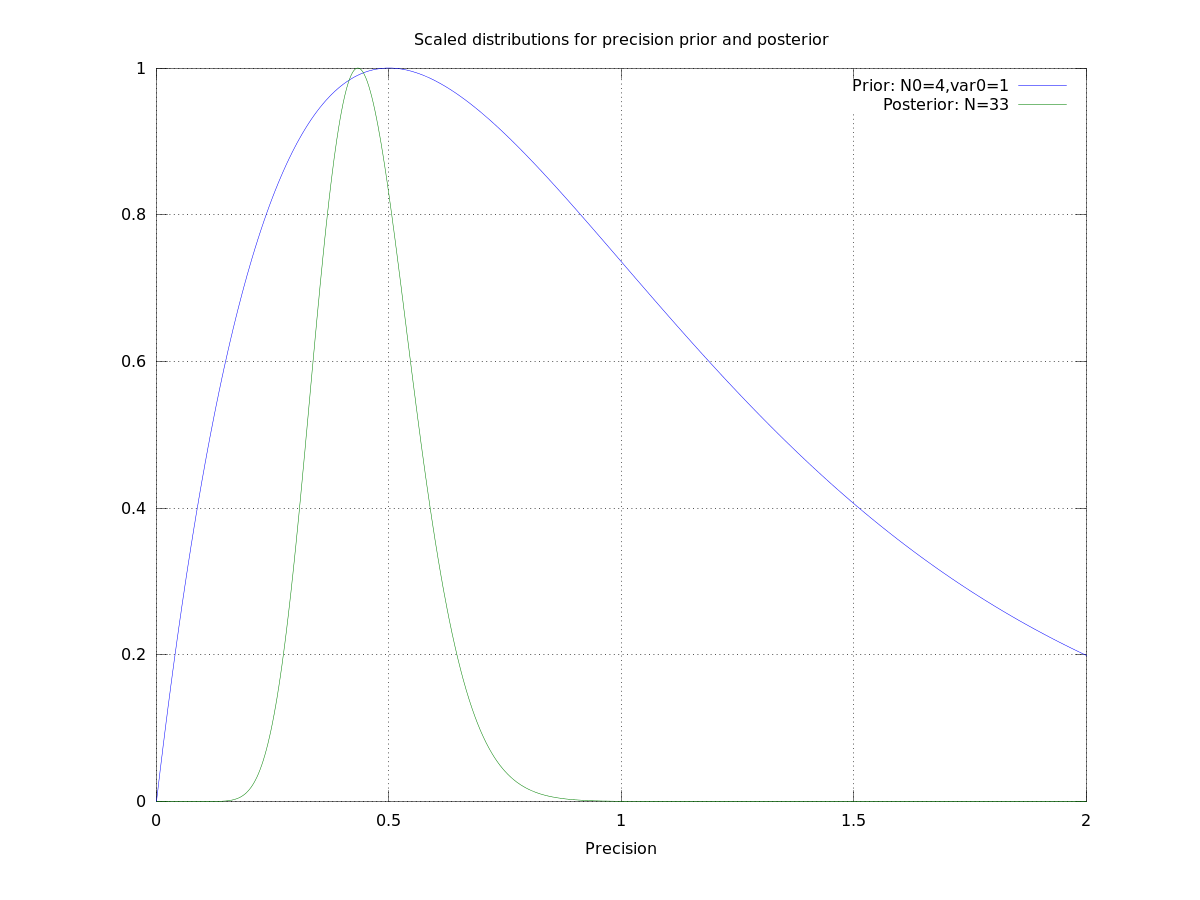
\includegraphics[height=5cm]{precision_prior_and_posterior_1d}
\par\end{centering}

\caption{Estimating the precision of a Gaussian: prior and posterior.}
\label{fig:prec_prior_and_posterior_1d}
\end{figure}


This is all very heart warming, but only applicable if $X$ is fully
observed. In the more general case we will need the full joint $p(X,\mu_{x},\Sigma_{X})$,
quite another kettle of fish.


\subsection{Wishart for the multi-variate case}

Since our RV is a matrix (instead of a vector), the covariance no
longer fits into a matrix, but now needs a 4-dimensional structure.


\section{The Gaussian-Wishart or alternatively Normal Inverse Wishart distribution}

The conjugate prior for the combined mean and precision/covariance
of the Gaussian distribution.


\subsection{Factor operations}
\begin{itemize}
\item Products/divisions with other Gaussians, Wisharts or Gaussian-Wisharts
seems to involve only the product/division of the Gaussian parts with
each other, and the Wishart parts with each other.
\item The marginal wrt $\mathbf{X}$ will be Gaussian, while the marginal
wrt both $\mathbf{\mu}$ and $\Sigma$ will be GW/NIW again, the only
two marginals I think we will need.
\item On the observation side we probably only need to bother with observing
$\mathbf{X}$, it seems unlikely that we will have a need for observing
$\mathbf{\mu}$ and $\Sigma$.
\item We probably can get along without damping.
\item I am still unsure about the normalisation. If the Gaussian part is
in canonical form it is inherently normalised. I suspect a similar
result will hold for the Wishart part.
\end{itemize}
See Murphy pg 125 and on for details. On the wish list for a fine
day.



From the Wiki page: ``The least informative, proper Wishart prior
is obtained by setting n = p.

The prior mean of $W_p(V, n)$ is $nV-1$. This implies that a good
choice for $V$ is $n\mathcal{S}_0$, where $\mathcal{S}_0$ is some
prior guess for the covariance matrix.''


\chapter{The Linear Gaussian (LG) distribution}

\section{Purpose}
In many situations we need the distribution $p(Y|X)$ with $X$ Gaussian
and $Y = AX+\text{ noise }$ - this is an LG. Note, this is not simply
a case of upfront initialising the distribution based on that of
$X$. This distribution is continuously adapting as the distribution of
$X$ is evolving.  A typical use is for instance in the state propagation
of a Kalman Filter.

\section{Ramifications}
Here are a couple of trip-ups to watch out for, all in some way
coupled to the basic distribution being conditional:
\begin{itemize}
\item Without that noise term the joint covariance matrix is singular,
  indeed of the same rank as that of $C_X$.
\item In a PGM we first have to receive (multiply with) a $p(X)$
  message, thereby changing the above to $p(X,Y)$ before we can
  accomplish anything. This means that the order of messages are
  important. I think we can get past this one by sending out a vacuous
  message if we are required to output a message before having
  received the conditioning input. The message scheduler should then
  pick up that no new news was generated, and move this factor to the
  back burner until is has more interesting news.
\item In a network (such as a Kalman Smoother) we might also receive
  opposite direction messages i.e. $p(Y)$. We need to formulate an
  appropriate way to handle this.
\end{itemize}

\section{Operators}

\begin{tabular}{lllll}
  Parameterisation         & Operator             & Result                   & Details & Notes\\ \hline
                           & Product              &                          &         & \parbox{0.3\textwidth}{}\\
                           & Divide               &                          &         & \parbox{0.3\textwidth}{}\\
                           & Sum-marginalise      &                          &         & \parbox{0.3\textwidth}{Integrate over subset}\\
                           & Max-marginalise      &                          &         & \parbox{0.3\textwidth}{Observe subset at mode}\\
                           & Observe/reduce       &                          &         & \parbox{0.3\textwidth}{}\\
                           & Normalise            &                          &         & \parbox{0.3\textwidth}{Note, $g$ matters now}\\
                           & Dampen               &                          &         & \parbox{0.3\textwidth}{}\\
                           & Distance             &                          &         & \parbox{0.3\textwidth}{}\\
                           & Sample               &                          &         & \parbox{0.3\textwidth}{}\\
\end{tabular}

\chapter{Affine transformations of Gaussian RVs with application to parameter estimation}


\section{MVGs as a network of Linear Gaussians (LG)}

We often work with situations where an RV $\bm{x}$ is
affinely\footnote{This is also commonly referred to as a linear
Gaussian.}  transformed to an RV $\bm{y}$ i.e.
\begin{align*}
  \bm{y}=\bm{A}^{T}\bm{x}+\bm{c}+\bm{\nu},
\end{align*}
where
$\bm{x}\sim\mathcal{N}(\mu_{\bm{x}},\bm{\,\Sigma}_{\bm{xx}})$,
$\bm{c}$ is an offset vector and
$\bm{\nu}\sim\mathcal{N}(\bm{0},\,\bm{\Sigma}_{\bm{\nu\nu}})$.  As you
will see below, the joint $p(\bm{x},\bm{y})$ is also a Gaussian --
this proves useful in many situations. We can therefore reinterpret a
linear Gaussian description as a full joint Gaussian. The description
below is in terms of vector RVs, but the scalar case is easily
extracted by merely setting the dimensions of the vector in question,
to unity.

\subsection{From a linear Gaussian to a joint Gaussian}

Let us first consider $\bm{y}'=\bm{A}^{T}\bm{x}+\bm{c}$.
It is easy to show that
\[
\bm{y}'\sim\mathcal{N}(\bm{\mu_{\bm{y}'}=}\bm{A}^{T}\bm{\mu_{\bm{x}}}+\bm{c},\,\bm{\Sigma}_{\bm{y'y'}}=\bm{A}^{T}\Sigma_{\bm{xx}}\bm{A}).
\]
When we consider $\bm{x}$ and $\bm{y}'$ jointly (or conditionally),
the situation degenerates because the one determines the other. For
instance
$p(\bm{y'|}\bm{x)}=\delta(\bm{y'}-(\bm{A^{T}}\bm{x}+\bm{c}))$.  After
adding the noise term $\bm{\nu}$ (same dimension as $\bm{y}$), we are
in business again. The distribution for $\bm{y}$
now becomes:

\[
\bm{y}\sim\mathcal{N}(\bm{\mu_{\bm{y}}=}\bm{A}^{T}\bm{\mu_{\bm{x}}}+\bm{c},\,\bm{\Sigma}_{\bm{yy}}=\bm{A}^{T}\Sigma_{\bm{xx}}\bm{A}+\bm{\Sigma}_{\bm{\nu\nu}}).
\]


To specify the full joint $p(\bm{x},\bm{y})$ we still need
to determine the joint covariance $\bm{\Sigma}_{\bm{xy}}$:

\begin{align*}
\bm{\Sigma}_{\bm{xy}}= & \mathbb{E}[(\bm{x}-\mu_{\bm{x}})(\bm{y}-\mu_{\bm{y}})^{T}\\
= & \mathbb{E}[(\bm{x}-\mu_{\bm{x}})(\bm{\bm{A}^{T}\bm{x}}+\bm{\bm{c}}+\bm{\bm{\nu}}-(\bm{A}^{T}\bm{\mu_{\bm{x}}}+\bm{c}))^{T}]\\
= & \mathbb{E}[(\bm{x}-\mu_{\bm{x}})(\bm{A}^{T}(\bm{\bm{x}}-\bm{\mu_{\bm{x}}})+\bm{\bm{\nu}})^{T}]\\
= & \mathbb{E}[(\bm{x}-\mu_{\bm{x}})(\bm{(\bm{\bm{x}}-\bm{\mu_{\bm{x}}}){}^{T}A}+\bm{\bm{\nu}}^{T})]\\
= & \Sigma_{\bm{xx}}\bm{A}.
\end{align*}
The joint density therefore is:

\begin{equation}
\left[\begin{array}{c}
\bm{x}\\
\bm{y}
\end{array}\right]\sim\mathcal{N}\left(\left[\begin{array}{c}
\bm{\mu_{\bm{x}}}\\
\bm{\bm{A}^{T}\bm{\mu_{\bm{x}}}+\bm{c}}
\end{array}\right],\left[\begin{array}{cc}
\Sigma_{\bm{xx}} & \Sigma_{\bm{xx}}\bm{A}\\
\bm{A}^{T}\Sigma_{\bm{xx}}\hspace{5mm} & \bm{A}^{T}\Sigma_{\bm{xx}}\bm{A}+\bm{\Sigma}_{\bm{\nu\nu}}
\end{array}\right]\right).  \label{eq:linGaussToGauss}
\end{equation}

If we know the parameters
$(\mu_{\bm{x}},\bm{\,\Sigma}_{\bm{xx}},\,\bm{A} \text{ and } \bm{\Sigma}_{\bm{\nu\nu}})$ of an affine Gaussian specification, we
can use Eq \ref{eq:linGaussToGauss} to determine the corresponding
joint Gaussian distribution. Note, in contrast to earlier lectures, we
now think of $\bm{x}$ as an RV, not just a constant serving as parameter
of $\bm{y}$.


\paragraph{Example:}

We have a random variable $\mu\sim\mathcal{N}(0,1)$, and a second
random variable $x\sim\mathcal{N}(\mu,2)$ (i.e. $x$ is an RV centered
around whatever the value of RV $\mu$ is). Find and sketch their joint
distribution $p(x,\mu)$:

In this case we have $x=1\Mu+0+\nu$ with $\nu\sim\mathcal{N}(0,2)$.
Therefore from Eq.~\ref{eq:linGaussToGauss} we get the joint as:

\begin{align*}
\left[\begin{array}{c}
\mu\\
x
\end{array}\right]= & \mathcal{N}\left(\left[\begin{array}{c}
0\\
0
\end{array}\right],\left[\begin{array}{cc}
1 & 1\\
1 & 3
\end{array}\right]\right).
\end{align*}


For later use we also calculate the precision matrix

\begin{align*}
J= & \left[\begin{array}{cc}
1.5 & -0.5\\
-0.5 & 0.5
\end{array}\right].
\end{align*}


See Fig \ref{fig:bayesmeanest}(a) for a plot of the joint distribution.


\paragraph{Example:}

For the previous example, we observe%
\footnote{The true mean used to generate the $x_{i}$ values was $\mu=1.5$.%
} the following values

\begin{align*}
x_{1\ldots10}= & (-0.45,1.68,0.49,2.29,2.65,3.10,0.89,0.90,0.25,-0.04).
\end{align*}


From this, determine the sequential (i.e. after the first observation,
then after the first two observations, etc.) ML, MAP and Bayesian
estimates for the distribution of $p(x|x_{1\ldots N_{i}})$ with
$N_{i}=1\ldots10$.

a) The ML estimate is simply the arithmetic mean of the observations:

\begin{align*}
\mu_{\mbox{MLE}}(x_{1\ldots N_{i}})= & \frac{\sum_{n=1}^{N_{i}}x_{n}}{N_{i}}.
\end{align*}


Sequentially (i.e. as we use more and more data) this gives the estimates:

\begin{align*}
\mu_{\mbox{MLE}}(x_{1\ldots N_{i}})= & (-0.450,0.615,0.573,1.003,1.332,1.627,1.521,1.444,1.311,1.176),
\end{align*}
with $N_i = 1,2, \ldots , 10$.

b) The MAP estimate of the mean is the $\mu$ that maximises

\begin{align*}
p(\mu)\prod_{i}p(x_{i}|\mu)= & \exp\left[-\frac{\mu^{2}}{2}-\sum_{i}\frac{(x_{i}-\mu)^{2}}{4}\right].
\end{align*}


Taking the log and setting the derivative wrt $\mu$ equal to zero
gives:

\begin{align*}
\mu_{\mbox{MAP}}(x_{1\ldots N_{i}})= & \frac{\sum_{n=1}^{N_{i}}x_{n}}{N_{i}+2}.
\end{align*}


In effect it is as if we had, in this case, two 'phantom' observations,
both placed at the mean of the prior i.e. at zero. Note that that
the variance of the prior dictates the number of 'phantom' observations.
The sequence of estimates (with growing $N_i)$ now changes to:

\begin{align*}
\mu_{\mbox{MAP}}(x_{1\ldots N_{i}})= & (-0.150,0.308,0.344,0.668,0.951,1.220,1.183,1.155,1.072,0.980).
\end{align*}


For both ML and MAP we work with point estimates, resulting in a distribution
for $x$ given by:

\begin{align*}
p(x|x_{1\ldots N_{i}})= & \mathcal{N}(\mu_{\mbox{est}}(x_{1\ldots N_{i}}),2).
\end{align*}


c) For the Bayesian estimate, lets start out with the graphical model
that describes $p(\mu,x|x_{1\ldots N})$:

\begin{figure}[!h]
  \hfill\begin{centering}
    \parbox{0.4\textwidth}{
      \centering
        \psfragfig*[height=6cm,crop=pdfcrop]{bayesianmean_BN} \\
        %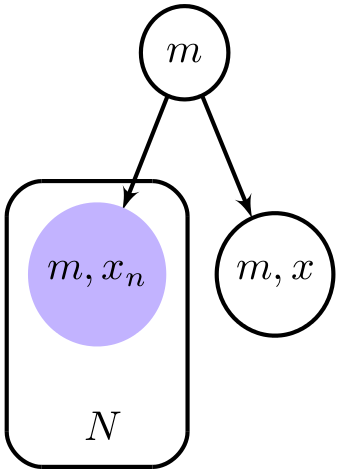
\includegraphics[width=3cm]{bayesianmean_BN} \\
      (a) Represented as a Bayes net.
    }
  \end{centering}\hfill
  %%%%%%%%%%%%%%
  \begin{centering}
    \parbox{0.4\textwidth}{ \centering
      \psfragfig*[height=6cm,crop=pdfcrop]{bayesianmean_CG} \\
      %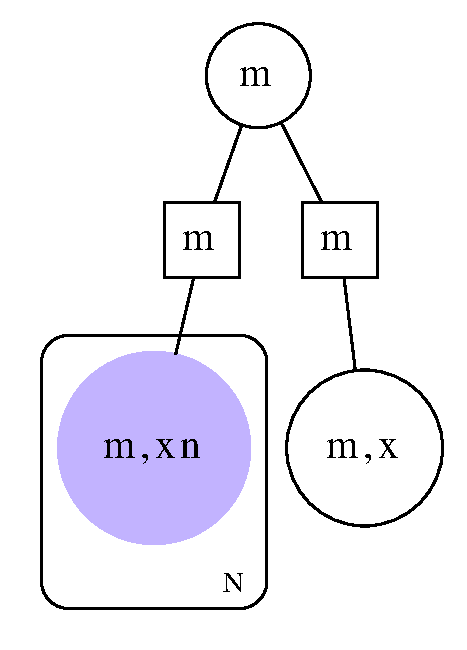
\includegraphics[width=3cm]{bayesianmean_CG}\\
 (b) Represented as a cluster graph ($\mu$ is unobserved).
}
  \end{centering} \hfill
  %%%%%%%%%%%%%%
\caption{Bayesian estimation of a mean given known covariance and
  prior. We include the extra unobserved $x$ because we are interested
  in the joint distribution of $x$ and $\mu$.}
  \label{fig:lingaus_graphs}
\end{figure}


Note from Fig. \ref{fig:lingaus_graphs}(a) that the joint
\begin{align*}
  p(\mu,x,x_{1\ldots N}) &= p(\mu) p(x|\mu)p(x_{n}|\mu).
\end{align*}
To keep things simple, we will use them in canonical form.

For the prior $p(\mu)$ the canonical parameters are:

\begin{align*}
\bm{K}_{\mu}= & \left[\begin{array}{cc}
1 & 0\\
0 & 0
\end{array}\right]\mbox{ and }\\
\bm{h}_{\mu}= & \left[\begin{array}{c}
0\\
0
\end{array}\right].
\end{align*}
The joint $p(\mu,x)$ we obtained in the previous example:

\begin{align*}
\bm{K}_{\mu,x}= & \left[\begin{array}{cc}
1.5 & -0.5\\
-0.5 & 0.5
\end{array}\right]\mbox{ and }\\
\bm{h}_{\mu,x}= & \bm{0}.
\end{align*}

With the conditional distributions of the form $p(x|\mu)$ we have to
be somewhat careful -- normally when we want a conditional
distribution we simply observe the value in the joint distribution and
that is it. However, in this case that will leave us with
$p(\mu|x_{n})$ which is not what we want. The problem arises because
the observed RV $x_{n}$ now is to the \emph{left} of the condition
bar, not in its usual place to the right of it. Either we have to
consider $\exp\left[-\sum_{n}\frac{(x_{n}-\mu)^{2}}{4}\right]$ as a
function of $\mu$ with known $x_{n}$'s, or we can equivalently
determine it via $p(x_{n}|\mu)=\frac{p(\mu,x)}{p(\mu)}.$ Using
canonical form division we get the corresponding canonical parameters
as:

\begin{align*}
\bm{K}_{x|\mu}= & \left[\begin{array}{cc}
0.5 & -0.5\\
-0.5 & 0.5
\end{array}\right]\mbox{ and }\\
\bm{h}_{x|\mu}= & \bm{0}.
\end{align*}


Note that $\bm{K}_{x|\mu}$ is singular, this should not be a surprise
since it describes a one-dimensional function. When we now observe a
particular $x_{n}$ this becomes (see Koller for the equations for
canonical form reduction):

\begin{align*}
\bm{K}_{x_{n}|\mu}= & \left[\begin{array}{cc}
0.5 & 0\\
0 & 0
\end{array}\right]\mbox{ and }\\
\bm{h}_{x_{n}|\mu}= & \left[\begin{array}{c}
0.5x_{n}\\
0
\end{array}\right].
\end{align*}

The canonical form of our full\footnote{Something interesting is
going on here with the inclusion of the $p(x|\mu)$ term and its effect
via $\bm{K}_{x|\mu}$. It does change the posterior very slightly --
only by omitting it do we get a posterior with its maximum exactly at
the MAP estimate point.} joint $p(\mu,x|x_{1\ldots N})$ is now given
by:

\begin{align*}
\bm{K}_{\mu,x|x_{1\dots N_{i}}}= & \bm{K}_{\mu}+\bm{K}_{x|\mu}+\sum_{n=1}^{N_{i}}\bm{K}_{x_{n}|\mu},\\
= & \left[\begin{array}{cc}
1.5+0.5N_{i} & -0.5\\
-0.5 & 0.5
\end{array}\right]\mbox{ and }\\
h_{\mu,x|x_{1\dots N_{i}}}= & \bm{h}_{\mu}+\bm{h}_{x|\mu}+\sum_{n=1}^{N_{i}}\bm{h}_{x_{n}|\mu}\\
= & \left[\begin{array}{c}
0.5\sum_{n=1}^{N_{i}}x_{n}\\
0
\end{array}\right].
\end{align*}


\begin{figure}
  \begin{centering}
  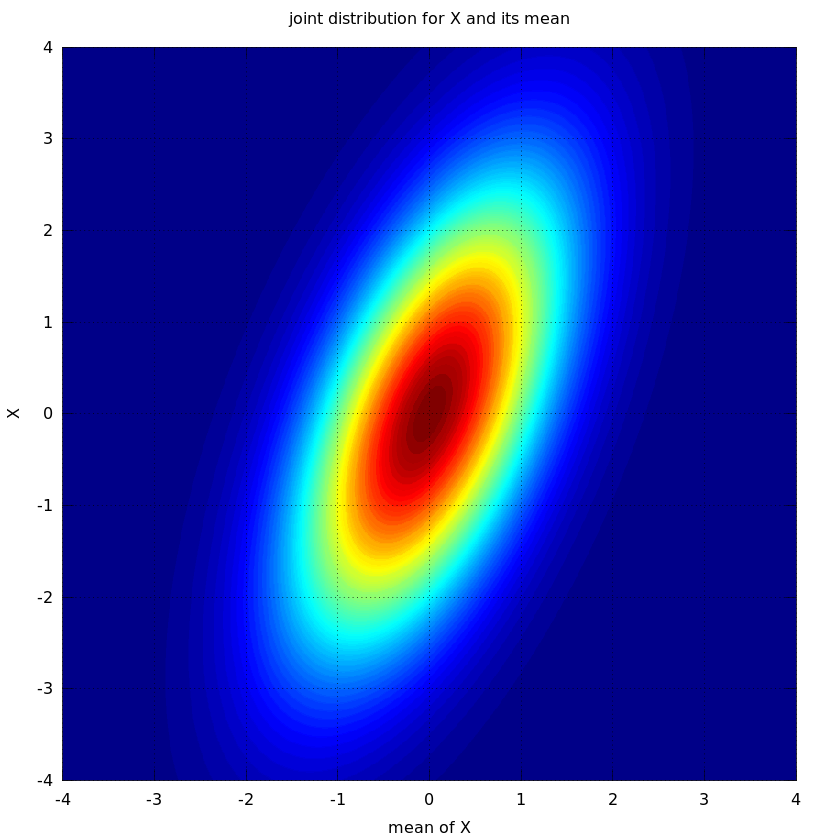
\includegraphics[width=6cm]{bayesmean0}\\
  (a) The joint $p(\mu,x)$. The correlation between $\Mu$ and $x$ is
  clear, vertical cuts shifts the conditional distribution $p(x|\mu)$.
  \end{centering}

  \begin{centering}
  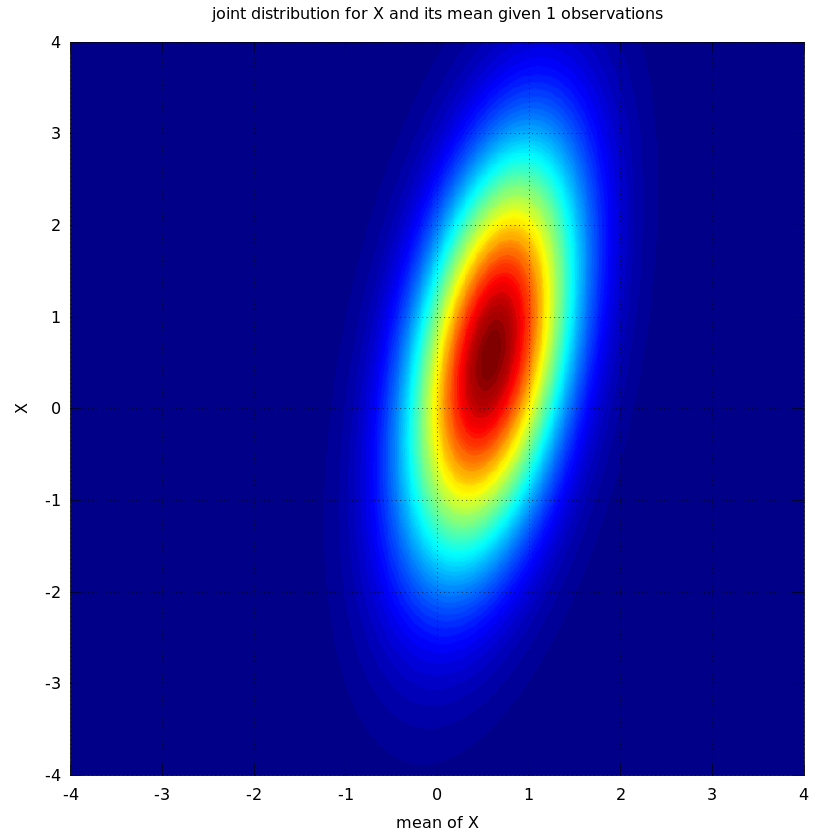
\includegraphics[width=6cm]{bayesmean1}\\
  (b) The joint $p(\mu,x|x_{1})$ (i.e. after taking one observation into
  account). A marked but controlled shift away from the prior, is evident.
  \end{centering}

  \begin{centering}
  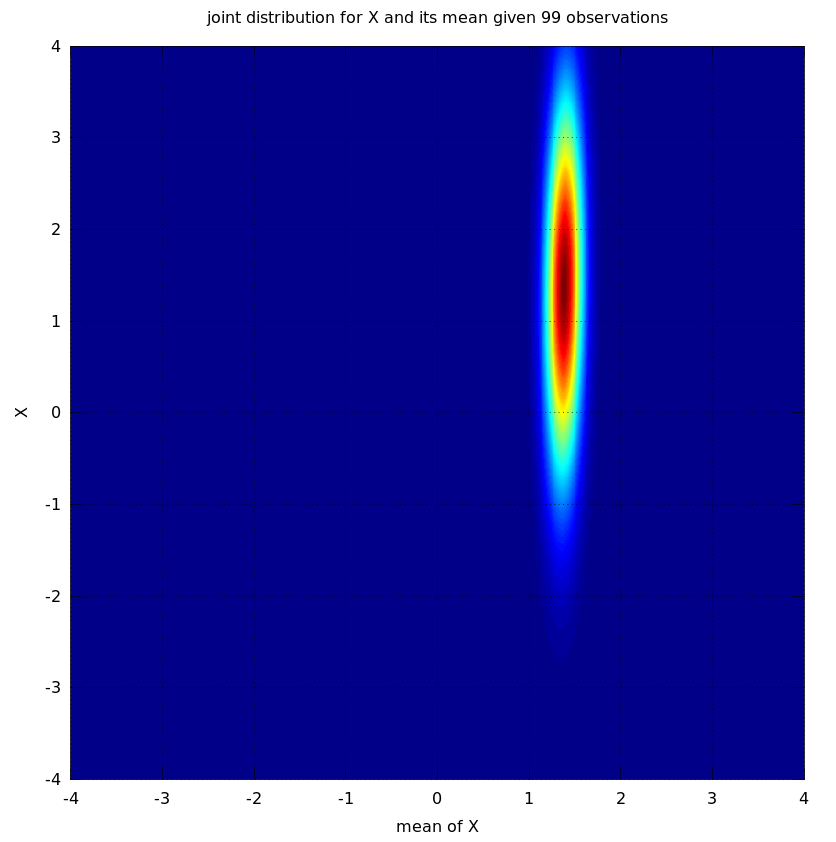
\includegraphics[width=6cm]{bayesmean99}\\
  (c) The joint $p(\mu,x|x_{1\ldots99})$ (i.e. after 99 observations).
  The estimate now lies quite close to the true underlying value (which
  was 1.5).
  \end{centering}

\caption{Bayesian estimation of the mean $\mu$ of RV $x$.}
\label{fig:bayesmeanest}
\end{figure}


Note how the inclusion of $\bm{K}_{\mu}$ on the right hand side
reverts the precision matrix to a non-singular
state. Fig. \ref{fig:bayesmeanest} shows how observing more and more
$x_{n}$ values refines our knowledge about the distribution of $\mu$.

\paragraph{Reflection:}

A subtly beautiful thing, worthwhile to reflect on, has happened here.

With the ML and MAP estimates, we designed a cost function (based
on the likelihood and prior information) and framed the problem as
estimating the \emph{single parameter point} that minimises the chosen
cost function. To do this we had to solve an \emph{optimisation} problem
-- this was quite easy for the Gaussians (it had a closed form), but
could be extremely hard for some other distributions. But if we substitute
for another set of observations, it will be different. And our point
estimate has no way to characterise this variability.

The central hard things to do in Bayesian estimates, are marginalisation
and observation. For the Gaussian the solution to these is provided
via the canonical form. We now change the problem from that of estimating
a parameter point, to estimating the \emph{distribution} of the parameters
given our prior knowledge and observations. We find this distribution,
not by optimising, but by doing inference, i.e. some form of message
passing in a graphical model. \emph{Learning now becomes inference!}
For this specific case the resultant PGM has a tree structure and
is therefore exactly solvable. In general it will have a graph structure
and we can approximately solve it using loopy belief propagation.
It can be shown \cite{Barber2012} that this is equivalent to approximate
the Bayesian estimate via variational inference\cite{MacKay2003}.
This generalising view of representing parameters by a distribution
instead of a point, makes the system much more resistant to overfitting.

In this specific case, our observations were also independent given
the parameters. We can therefore also cast this into a sequential
Bayesian estimation where we combine the prior and the first observation
to estimate a posterior distribution for the parameters (a very simple
PGM). This posterior then becomes the prior for the second observation
etc., we keep on iterating the process as we acquire more and more
information.


\subsection{From a joint Gaussian to a linear Gaussian}

It is also useful to reduce a full Gaussian description to linear
Gaussian. If we have the full Gaussian distribution available as:

\[
\left[\begin{array}{c}
\mathbf{X}\\
\mathbf{Y}
\end{array}\right]\sim\mathcal{N}\left(\left[\begin{array}{c}
\mathbf{\mu_{\mathbf{X}}}\\
\mathbf{\mu_{\mathbf{Y}}}
\end{array}\right],\left[\begin{array}{cc}
\Sigma_{\mathbf{XX}} & \Sigma_{\mathbf{XY}}\\
\Sigma_{\mathbf{YX}}=\Sigma_{\mathbf{XY}}^{T}\hspace{5mm} & \Sigma_{\mathbf{YY}}
\end{array}\right]\right),
\]
 we can find the corresponding linear Gaussian parameters as follows:

Firstly, $\mu_{\mathbf{X}}$ and $\Sigma_{\mathbf{XX}}$ are directly
known from the full covariance description. We can determine $\mathbf{A}$
from the covariance term:

\begin{align}
\Sigma_{\mathbf{XY}}= & \Sigma_{\mathbf{XX}}\mathbf{A}\nonumber \\
\therefore\mathbf{A}= & \Sigma_{\mathbf{XX}}^{-1}\Sigma_{\mathbf{XY}}.
\end{align}


With that known, $\mathbf{c}$ is easily solved by comparing the means:

\begin{equation}
\mathbf{c}=\mu_{\mathbf{Y}}-\mathbf{A}^{T}\mathbf{\mu_{\mathbf{X}}}.
\end{equation}
Finally we solve the noise covariance as:

\begin{align}
\mathbf{\Sigma}_{\mathbf{NN}}= & \Sigma_{\mathbf{YY}}-\mathbf{A}^{T}\Sigma_{\mathbf{XX}}\mathbf{A}\nonumber \\
= & \Sigma_{\mathbf{YY}}-\mathbf{A}^{T}\Sigma_{\mathbf{XY}}.
\end{align}



\subsection{Ponderings on generalising to more dependencies }

NOTE: You can easily skip this bit, I was just exploring for a moment
to see where it might lead. And my conclusion is ``nowhere special''.

Let us now generalise to the case where $\mathbf{Y}$ is dependent
on multiple $\mathbf{X}_{i}'s$ i.e.

\[
\mathbf{Y}=\mathbf{\sum_{i=1}^{N}A_{i}}^{T}\mathbf{X_{i}}+\mathbf{c_{i}}+\mathbf{N_{i}},
\]
with each $\mathbf{X_{i}}\sim\mathcal{N}(\mu_{i},\mathbf{\,\Sigma}_{ii})$
and $\mathbf{N_{i}}\sim\mathcal{N}(\mathbf{0},\, R_{ii})$ distinct
and independent of the others.

We can visualize this as a Bayes net, shown in Fig \ref{fig:lingauss_bn}.
Note that, with $\mathbf{Y}$ unobserved, all the $\mathbf{X}_{i}$'s
are statistically independent from each other. However, when $\mathbf{Y}$
is known, they all become conditionally dependent on each other. I.e.
the moralizing process involved when converting from a Bayes-net to
a Markov-random-field, will tie all these variables into one (large)
cluster/clique, irrespective of whether $\mathbf{Y}$ was observed
or not. These general independencies unfortunately does not necessarily
imply conditional independencies - the information might still be
dense in spite of a very sparse covariance matrix.

\begin{figure}
\noindent \begin{centering}
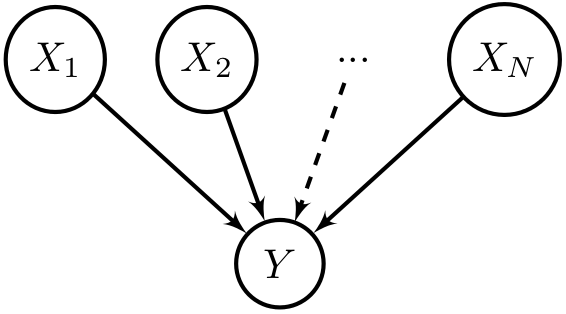
\includegraphics[height=3cm]{lingauss_bn}
\par\end{centering}

\caption{General linear Gaussian.}
\label{fig:lingauss_bn}
\end{figure}


The full Gaussian describing this situation is given by:

\begin{equation}
\left[\begin{array}{c}
\begin{array}{c}
\mathbf{X}_{1}\\
\vdots\\
\vdots\\
\mathbf{X}_{N}\\
\mathbf{Y}
\end{array}\end{array}\right]\sim\mathcal{N}\left(\left[\begin{array}{c}
\mathbf{\mu}_{1}\\
\vdots\\
\vdots\\
\mathbf{\mu}_{N}\\
\mathbf{\mathbf{\sum_{i=1}^{N}A_{i}}^{T}\mathbf{\mu_{i}}+\mathbf{c_{i}}}
\end{array}\right],\left[\begin{array}{ccccc}
\Sigma_{11} & \mathbf{0} & \hdots & \mathbf{0} & \Sigma_{11}\mathbf{A}_{1}\\
\mathbf{0} & \ddots & \ddots & \vdots & \vdots\\
\vdots & \ddots & \ddots & \mathbf{0} & \vdots\\
\mathbf{0} & \hdots & \mathbf{0} & \Sigma_{NN} & \Sigma_{NN}\mathbf{A}_{N}\\
\mathbf{A}_{1}^{T}\Sigma_{11} & \hdots & \hdots & \mathbf{A}_{N}^{T}\Sigma_{NN} & \hspace{5mm}\sum_{i=1}^{N}\mathbf{A}_{i}^{T}\Sigma_{ii}\mathbf{A}_{i}+\mathbf{R}_{ii}
\end{array}\right]\right).
\end{equation}


Note the blocks of zeros in the covariance matrix, these indicates
that the corresponding random vectors are independent \emph{if $\mathbf{Y}$}
is not known. The equations for determining the linear Gaussian parameters
from the full covariance description now becomes:

\begin{eqnarray}
\mathbf{A}_{i} & = & \Sigma_{ii}^{-1}\Sigma_{i\mathbf{Y}},\\
\sum_{i=1}^{N}\mathbf{c}_{i} & = & \mu_{\mathbf{Y}}-\sum_{i=1}^{N}\mathbf{A}_{i}^{T}\mathbf{\mu}_{i},\mbox{ and}\\
\sum_{i=1}^{N}\mathbf{R}_{ii} & = & \Sigma_{\mathbf{YY}}-\sum_{i=1}^{N}\mathbf{A}_{i}^{T}\Sigma_{i\mathbf{Y}}.
\end{eqnarray}


Note that with both $\mathbf{c}_{i}$ and $\mathbf{R}_{ii}$ we have
some extra freedom. However, the covariances must still remain symmetric
and positive definite.


\section{MVGs as a network of bi-variate Gaussians (BVGs)}


\subsection{The general idea}

Representing a multi-variate Gaussian as a network of two-dimensional
Gaussians can be very useful. Amongst others this simplifies the required
operations such as inversion etc greatly. The likely price to pay
is that the resultant structure will be loopy. Is this doable? The
short answer is a qualified yes, Koller \cite[Section 14.2.3]{Koller2009}
shows how. However, her solution has a few aspects that might not
work well with our EMDW implementation:
\begin{itemize}
\item The solution is explicitly framed as a factor graph whereas we prefer
to work with cluster graphs. Of course, with variable pairs, the graph
will always implicitly end up as being a factor graph but, instead
of dictating it from the outside, we prefer EMDW to do the configuration
automatically. In the interaction with other MVGs, things might go
wrong.
\item She breaks the graph up into a number of pairwise factors, and a number
of single factors. However, the pairwise factors can not stand on
their own legs, they \emph{must }receive their messages from the single
factors before they are able to send out their own messages. This
just might cause trouble in a loopy system if we do not explicitly
specify the message passing order beforehand -- I'm also unsure as
to how well this will work with an initial vacuous canonical form.
\end{itemize}
The approach we develop here directly models the MVG as a network
of BVG's where each BVG is a fully functional Gaussian distribution.
Fig. \ref{fig:gaussianpairs_cg} illustrates the resulting structure
as a cluster graph of BVGs. The illustration is for the five-dimensional
case, but how to extend it to arbitrary dimensions is clear. Such
a network will consist of $\frac{D(D-1)}{2}$ BVG nodes, with $D$
the number of variables represented by the MVG. Although we show the
full connected cluster graph structure (obeying the RIP property),
in general we will not concern ourselves with linking the BVG factors
-- in the EMDW system that is handled automatically by the code. If
the MVG information matrix $J$ has zeros in some locations, the corresponding
BVG terms disappear, thereby simplifying the cluster graph.

\begin{figure}
\noindent \begin{centering}
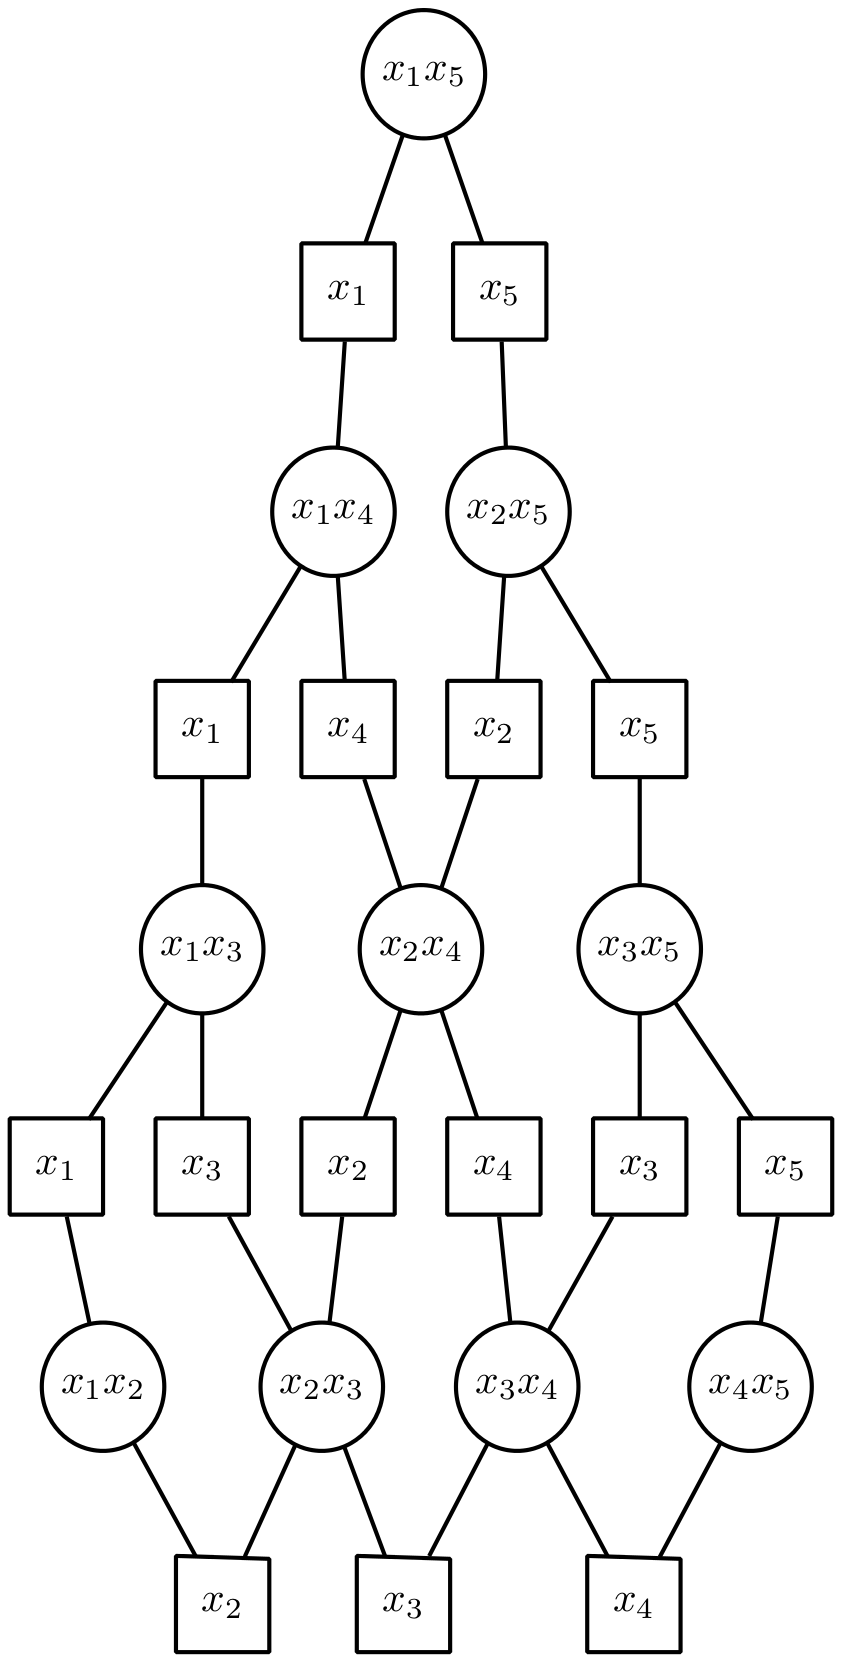
\includegraphics[height=10cm]{gaussian_pairs}
\par\end{centering}

\caption{Representing a multi-variate Gaussian on $X_{1}\hdots X_{5}$ as a
cluster graph with pairwise clusters.}
\label{fig:gaussianpairs_cg}
\end{figure}


We will find that such a structure is indeed adequate for representing
a general MVG. However, the BVGs are not uniquely specified, and the
requirement that their covariance matrices be symmetric and positive
definite, will introduce a constrained optimization as a subtask in
configuring them. Fortunately this is only necessary when initially
setting up the network, during the subsequent inference procedure
the message passing do not change the scope of the the BVGs and processing
is quite efficient.

Since both BVGs and 1VGs are just a special case of the MVG, there
also should be no limitation on combining them in a network.

To fix ideas, we are below first going to investigate the three-dimensional
case, and after that generalise to the $d$-dimensional case.


\subsection{Representing a three-dim Gaussian as three two-dim Gaussians \label{sub:Representing-a-three-dim}}


\subsubsection{From a product of three BVGs to an three-dim MVG}

Consider the product of generic canonical forms $\mathcal{C}(x,y;K_{1,2},\mathbf{h}_{1,2})\mathcal{C}(y,z;K_{2,3},\mathbf{h}_{2,3})\mathcal{C}(x,z;K_{1,3},\mathbf{h}_{1,3})$.
The identifying subscripts were chosen with some advance knowledge,
for now simply accept them as such. It covers all the pairwise connections
if we were to work with three RVs $X,Y\mbox{ and }Z$. We first have
to extend the three scopes to a common one. The information matrices
then become:

\begin{align*}
K_{1,2}= & \left[\begin{array}{ccc}
K_{1,2}^{x,x} & K_{1,2}^{x,y} & 0\\
K_{1,2}^{y,x} & K_{1,2}^{y,y} & 0\\
0 & 0 & 0
\end{array}\right],\\
K_{2,3}= & \left[\begin{array}{ccc}
0 & 0 & 0\\
0 & K_{2,3}^{y,y} & K_{2,3}^{y,z}\\
0 & K_{2,3}^{z,y} & K_{2,3}^{z,z}
\end{array}\right],\\
K_{1,3}= & \left[\begin{array}{ccc}
K_{1,3}^{x,x} & 0 & K_{1,3}^{x,z}\\
0 & 0 & 0\\
K_{1,3}^{z,x} & 0 & K_{1,3}^{z,z}
\end{array}\right].
\end{align*}


The potential vectors become:

\begin{align*}
\mathbf{h}_{1,2}= & \left[\begin{array}{c}
h_{1,2}^{x}\\
h_{1,2}^{y}\\
0
\end{array}\right],\\
\mathbf{h}_{2,3}= & \left[\begin{array}{c}
0\\
h_{2,3}^{y}\\
h_{2,3}^{z}
\end{array}\right],\\
\mathbf{h}_{1,3}= & \left[\begin{array}{c}
h_{1,3}^{x}\\
0\\
h_{1,3}^{z}
\end{array}\right].
\end{align*}
Since the $g$'s are scalar, they remain unchanged. Then we can apply
the rule for the product of canonical forms (Eq \ref{eq:cfprod})
to obtain (we identify it with an $\mbox{MVG}$ subscript in anticipation
of its later use):

\begin{align}
K_{\mbox{\mbox{MVG}}}= & \left[\begin{array}{ccc}
K_{1,3}^{x,x}+K_{1,2}^{x,x}\hspace{5mm} & K_{1,2}^{x,y} & K_{1,3}^{x,z}\\
K_{1,2}^{y,x} & K_{1,2}^{y,y}+K_{2,3}^{y,y}\hspace{5mm} & K_{2,3}^{y,z}\\
K_{1,3}^{z,x} & K_{2,3}^{z,y} & K_{2,3}^{z,z}+K_{1,3}^{z,z}
\end{array}\right],\\
\mathbf{h}_{\mbox{\mbox{MVG}}}= & \left[\begin{array}{c}
h_{1,3}^{x}+h_{1,2}^{x}\\
h_{1,2}^{y}+h_{2,3}^{y}\\
h_{2,3}^{z}+h_{1,3}^{z}
\end{array}\right],\mbox{ and }
\end{align}


This then shows the relationship between the parameters of the three
two-dim Gaussians, and that of their product.
\begin{itemize}
\item Note the one-to-one relationship of the off-diagonal terms of the
MVG to the off-diagonal terms of the BVGs -- they uniquely specify
each other.
\item However, from the summations in the diagonal terms of $K_{\mbox{MVG}}$
it is clear that the diagonal terms of the BVG information matrices
are not uniquely determined. However, this allocation will also have
to take into account that these covariances \emph{must }be symmetric
and positive definite.
\item In allocating values to $\mathbf{h}_{i}$ we also have some freedom
-- in this case there does not seem do be any special restrictions.
It should be safe to, for instance, simply split them equally.
\end{itemize}

\subsubsection{Equivalency of an MVG to a product of BVGs}

Clearly the product of BVGs is an MVG. Is this fully generic in the
sense that we can represent any MVG as the product of BVGs? Intuitively
one would think so, but unfortunately this is not so.


\paragraph{Definitions: Attractive and Diagonally Dominant:}

Symmetric matrices that are either attractive or diagonally dominant,
are guaranteed to be positive definite \cite[p 256]{Koller2009}. However,
although \emph{sufficient}, these conditions are not \emph{necessary}
for positive definiteness.
\begin{itemize}
\item According to Koller a matrix $J$ is said%
\footnote{This does not make sense to me. However, the partial correlation between
$i$ and $j$ is $\frac{-J_{i,j}}{\sqrt{J_{i,i}J_{j,j}}}$ and I presume
its absolute value should be less than one. My guess is what was intended
is: $|J_{i,j}|<\sqrt{J_{i,i}J_{j,j}}$. In similar vein I wonder if
for a covariance matrix a useful test for validity would be that the
magnitude of all correlation coefficients $|\rho_{i,j}|<1$ i.e. $|\sigma_{i,j}|<\sigma_{i}\sigma_{j}$.%
} to be attractive if, for all $i\neq j$: $-J_{i,j}\geq\sqrt{J_{i,i}J_{j,j}}$.
\item A matrix $J$ is said to be diagonally dominant if, for all%
\footnote{Personally I suspect that it will still be guarranteed positive definite
if we also allow equality for all but one of the diagonals.%
} $i$: $\sum_{j\neq i}|J_{i,j}|<J_{i,i}$.
\end{itemize}
Let us now consider the following information matrix (still from Koller):

\begin{align*}
J= & \left[\begin{array}{ccc}
1 & 0.6 & 0.6\\
0.6 & 1 & 0.6\\
0.6 & 0.6 & 1
\end{array}\right].
\end{align*}


Although neither diagonally dominant nor attractive, this matrix still
is positive definite with eigenvalues $\{0.4,0.4,2.2\}$ and $|J|=0.352$.
It therefore is a valid MVG information matrix. But it is not possible
to write this as the product of three BVGs. Bummer.

Is this particular to the way we parameterize our MVN as multiple
BVGs? If I consider the way that Koller parameterizes (see pg 255
and 613), after all messages have been multiplied in you are exactly
in this same situation and the same problem will apply. So, I don't
think so. Fortunately this problem should only crop up when initially
setting the network up, after that it should be ok.

From this we deduce that \emph{a product of BVGs can only model a
subset of the distributions MVGs can}. Which subset? I'm sure that
this must be known, but at the moment I'm in the dark about this.
My initial guess is that it might be exactly those where $J$ is constrained
to be diagonally dominant (for instance reduce the cross-terms to
0.5 in the above example). But, as yet, I have not proven this.

This result holds an important implication -- although BVGs have many
nice properties (easy inversion etc), if we want to work with arbitrary
Gaussians we will need to supplement them with MVGs.

Another interesting possibility is to extend the BVGs with some 3VGs
(and even higher dim Gaussians as is necessary) to do the factorisation.
Here there still is a lot of unknowns to me -- how many of what order
Gaussians will be necessary to model a particular high-dim Gaussian.
Does it depend on the number of places where $J$ fails being diagonally
dominant? My personal guess is that:
\begin{itemize}
\item with one diagonal index $i$ not satisfying diagonal dominance, will
call for using 3VGs combining variables $(i,j,k)$ where $(j,k)$
should cover all combinations of variables interacting with $i$.
Any BVGs defined on any two of these indices are removed since they
will also be covered by this 3VG.
\item if there is a second contravention at $p$, the same will be required
for variables $(p,q,r)$. Whenever two of these indices coincide with
a previously defined Gaussian, for instance on $(i,q,r)$, we will
probably need to replace both these 3VGs with a 4VG on $(i,p,q,r)$
etc. But there is a lot of detail to figure out here. Have a look
at Gaussians with precision matrices such as: $\begin{array}{ccc}
1.00000 & 0.60000 & 0.60000\\
0.60000 & 1.00000 & 0.60000\\
0.60000 & 0.60000 & 1.00000
\end{array}$or $\begin{array}{cccc}
1.00000 & 0.40000 & 0.40000 & 0.40000\\
0.40000 & 1.00000 & 0.40000 & 0.40000\\
0.40000 & 0.40000 & 1.00000 & 0.40000\\
0.40000 & 0.40000 & 0.40000 & 1.00000
\end{array}$. They are positive definite, but not diagonally dominant. Try and
express them as product of valid 2-dim Gaussians! How about 3-dim?
One can also relax this slightly by only breaking diagonal dominance
at a specific diagonal instead of everywhere. Something like: $\begin{array}{cccc}
1.00000 & 0.40000 & 0.40000 & 0.40000\\
0.40000 & 1.00000 & 0.20000 & 0.20000\\
0.40000 & 0.20000 & 1.00000 & 0.20000\\
0.40000 & 0.20000 & 0.20000 & 1.00000
\end{array}$. I suspect this one can be represented as the product of three valid
3-dim Gaussians.
\end{itemize}

\subsubsection{From a three-dim MVG to a product of BVGs}


\paragraph{Example (continued):}

To remind ourselves, our earlier example was 3-dim Gaussian with:

\begin{align*}
K_{\mbox{MVG}}= & \left[\begin{array}{rrr}
0.3125 & -0.125 & 0\\
-0.125 & 0.5833 & 0.3333\\
0 & 0.3333 & 0.3333
\end{array}\right]\\
\mathbf{h_{\mbox{MVG}}}= & \left[\begin{array}{r}
0.68750\\
-0.5416???7\\
0.33333
\end{array}\right].
\end{align*}


$|K_{\mbox{MVG}}|=0.020833$, therefore it is positive definite as
is required of a valid information matrix. Two of the diagonal values
are dominant, and the last one is just on the boundary of being so.
Importantly, also note that $K_{\mbox{MVG}}^{1,3}=0$. This implies
that we do not need to model $p(x,z)$, i.e $K_{1,3}=\mathbf{h}_{1,3}=g_{1,3}=0$
. Now lets first consider the positive definiteness of the $K_{i}'s$.
In this specific case the only ambiguity comes from the $0.5833=K_{1,2}^{y,y}+K_{2,3}^{y,y}$
relationship. We can (easily) evaluate the positive definiteness via
the determinant: $|K|=K^{1,1}K^{2,2}-2K^{1,2}$. From this the smallest
value that will still keep $K_{1,2}$ positive definite, is $K_{1,2}^{y,y}>\frac{0.125^{2}}{0.3125}=0.05$,
and similarly for $K_{2,3}$ we need $K_{2,3}^{y,y}>0.3333$. This
leaves us with plenty of margin, a safe choice will be $K_{1,2}^{y,y}=0.15$
and $K_{2,3}^{y,y}=0.4333.$ (With only one source of ambiguity the
solution was easy here, in the next section we consider a more general
approach for this.) From this we get the (non-uniquely) chosen reduced
BVG canonical forms as:

\begin{align*}
K_{1,2}= & \left[\begin{array}{cc}
0.3125 & -0.125\\
-0.125 & 0.15
\end{array}\right],\\
K_{2,3}= & \left[\begin{array}{cc}
0.4333 & 0.3333\\
0.3333 & 0.3333
\end{array}\right],\\
\mathbf{h}_{1,2}= & \left[\begin{array}{c}
0.68750\\
-0.27083
\end{array}\right],\\
\mathbf{h}_{2,3}= & \left[\begin{array}{c}
-0.27083\\
0.3333
\end{array}\right].
\end{align*}


Translated to the covariance form this gives the two BVG distributions
as:

\begin{align*}
p(x,y) & \sim\mathcal{N}\left(\left[\begin{array}{c}
2.21668\\
0.04170
\end{array}\right],\left[\begin{array}{cr}
4.8 & 4\\
4 & 10
\end{array}\right]\right)\mbox{ and }\\
p(y,z) & \sim\mathcal{N}\left(\left[\begin{array}{r}
-6.0413\\
7.0413
\end{array}\right],\left[\begin{array}{rr}
10 & -10\\
-10 & 13
\end{array}\right]\right).
\end{align*}



\subsection{General procedure to reduce an MVG to a network of BVGs}

We now generalise the above to MVGs of arbitrary dimensions. (I suspect
this holds at least for the case of diagonally dominant matrices.)


\subsubsection{Determine the applicable BVGs }

Specify the original MVG as a canonical form $\mathcal{C}(\mathbf{x};K_{\mbox{MVG}},\mathbf{h}_{\mbox{MVG}})$.
Inspect the upper triangle of $K_{\mbox{MVG}}$ for terms that are
non-zero%
\footnote{For the cases where $K_{\mbox{MVG}}(i,j)=0$ the corresponding BVG
canonical forms are $K_{i,j}=\mathbf{h}_{i,j}=g_{i,j}=0$ and thus
discarded. If, however, all the off-diagonals in a row are zero, that
variable is conditionally independent of all the others and need to
be modelled by an univariate Gaussian (UVG).%
}. For each such a $K_{\mbox{MVG}}^{i,j}\neq0,\; j>i$, we want to
find a BVG $\mathcal{C}(\mathbf{x}_{i,j};K_{i,j},\mathbf{h}_{i,j})$.
To make the reasoning easier to understand, in the following we extend
the $K_{i,j}$'s to the full dimension of $K_{\mbox{MVG}}$ in the
same manner as we did in Section \ref{sub:Representing-a-three-dim}.


\subsubsection{Determining the information matrices $K_{i,j}$}

$K_{i,j}$ is the information matrix for the BVG describing the relationship
between $x_{i}$ and $x_{j}$. It has four non-zero cells, we will
denote them by:

\begin{align*}
K_{i,j}= & \left[\begin{array}{ccccc}
\mathbf{0} & \mathbf{0} & \mathbf{\mathbf{0}} & \mathbf{0} & \mathbf{0}\\
\mathbf{0} & K_{i,j}^{i,i} & \mathbf{0} & K_{i,j}^{i,j} & \mathbf{0}\\
\mathbf{0} & \mathbf{0} & \mathbf{0} & \mathbf{0} & \mathbf{0}\\
\mathbf{0} & K_{i,j}^{j,i} & \mathbf{0} & K_{i,j}^{j,j} & \mathbf{0}\\
\mathbf{0} & \mathbf{0} & \mathbf{0} & \mathbf{0} & \mathbf{0}
\end{array}\right]
\end{align*}


where the superscripts denote the RVs concerned, and the subscripts
identify the specific BVG.

The off-diagonal terms are easy:

\begin{align}
K_{i,j}^{i,j}=K_{i,j}^{j,i}= & K_{\mbox{MVG}}(i,j).
\end{align}


The diagonal terms are where it becomes tricky:

\begin{align}
K_{\mbox{MVG}}^{i,i}=\sum_{j\neq i} & K_{\min(i,j),\max(i,j)}^{i,i}.
\end{align}


We can have upto $D-1$ BVG information matrices in each such summation.
At the same time each of these BVG matrices must remain positive definite,
otherwise it can not be a valid normalizable distribution. We can
(possibly?) cast this as a constrained optimization problem, or opt
for a more heuristic approach. To ensure positive definiteness we
have to satisfy one of two conditions\cite[p 255]{Koller2009}:
\begin{description}
\item [{Direct~calculation:}] $K_{i,j}^{i,i}K_{i,j}^{j,j}>2K_{i,j}^{i,j}$
-- by definition necessary and sufficient.
\item [{Diagonally~dominant:}] $K_{i,j}^{i,i}>|K_{i,j}^{i,j}|\mbox{ and }K_{i,j}^{j,j}>|K_{i,j}^{i,j}|$
-- a good guess sufficient condition.
\end{description}
The following is my pragmatic first guess as to how to do this --
we still have to verify it in practice. In the following, bear in
mind that each $K_{i,j}$ participates in two summations, one towards
$K_{\mbox{MVG}}^{i,i}$ and one towards $K_{\mbox{MVG}}^{j,j}$.
\begin{itemize}
\item Allocate from $K_{\mbox{MVG}}$ diagonal terms to the corresponding
$K_{i,j}$ diagonal terms -- fully when there is only one term in
the sum, or just enough value to satisfy the diagonal dominance test
when we have several terms in the sum.
\item Now check all the $K_{i,j}$'s for those who have positive determinants.
Reduce their determinants to zero by partly returning diagonal values
to the lower of $K_{\mbox{MVG}}^{i,i}$ or $K_{\mbox{MVG}}^{j,j}$.
After this all $|K_{i,j}|=0$.
\item Now we want to roughly equalize the $K_{\mbox{MVG}}^{i,i}$'s. We
do this by repeatedly finding the lowest $K_{\mbox{MVG}}^{i,i}$,
identify its associated $K_{i,j}$'s and for each of them find their
associated $K_{\mbox{MVG}}^{j,j}$. Starting from the biggest of these,
increase the value of $K_{i,j}^{j,j}$ and correspondingly reduce
the value of $K_{i,j}^{i,i}$, passing the difference on to $K_{\mbox{MVG}}^{i,i}$.
At this point all $|K_{i,j}|=0$, while the $K_{\mbox{MVG}}^{i,i}$'s
are approximately of same size (we could also refine by taking the
number of terms in the sum also into account).
\item If at this point you have negative $K_{\mbox{MVG}}^{i,i}$ terms,
give up and use an MVG. Or go drink beer%
\footnote{And ponder other ways to factorize it -- maybe BVG-TriVG combinations?%
}. When you feel better, use an MVG. As said before, sometimes an MVG
just can't be converted to BVGs.
\item Now take the surplus value still available in the diagonal terms of
$K_{\mbox{MVG}}$ and divide the spoils between participating $K_{i,j}$'s.
This will boost the positive definiteness of the benefitting BVGs.
\end{itemize}
After positive definite $K_{i,j}$'s have been determined, we can
strip all the padding zeros to remain with the information matrix
for those particular two RVs.


\subsubsection{Determine the potential vectors $\mathbf{h}_{i,j}$.}

Once the $K_{i,j}$'s are in place, this is dead easy. Simply divide
the capacity however you see fit.


\subsection{General procedure to reduce an MVG to a product of lower dimensional
Gaussians}


\chapter{Representing distribution via Sigma-Points}


\section{Introduction}


\section{Factor operations}


\subsection{Dependencies: Transformations (QED)}

This is what sigma points were originally developed for and here they
can really shine. You simply get the sigma points for your input variable/vector
$X$, for each one of them apply the transformation to it to get the
corresponding sample in the space of $Y$, and from the combined set
of samples for $(X,Y)$, calculate a joint parametric representation
$p(X,Y)$. It is important though to match the type of distribution
of the joint to the properties of the transformation. For instance,
with $X$ a Gaussian, and $Y$ some monotonic transformation of it,
it probably makes sense to also use a Gaussian for the joint. If,
however, the transformation was non-monotonic, one should first determine
an appropriate target distribution type, possibly via laborious mathematical
derivation. For instance, if $Y=X^{2}$ the target distribution for
$Y$ should be Wishart/Gamma/Chi-squared, and the joint probably a
Gaussian-Wishart.


\subsection{Conditional Dependencies (QED)}

This one is a special case of the above mentioned transformations
-- the difference being that we now only know the transformation as
a distribution. If we have some prior distribution (including its
sigma points) for a parameter of the target density, we can predict
samples from the target density by means of each of these sigma points.
Maybe it is best to explain via an example.

\textbf{Example:} For instance, if we have a Gaussian prior for the
mean $\mu_{X}$ of a Gaussian RV $X$, the sigma points from $p(\mu_{x})$
are possible centroids around which samples of $X$ should be scattered.
But in contrast to the fixed transformations we encountered in the
previous section, we now will have a number of target samples associated
with each of the original sigma points. The original sigma-point weight
should now also be subdivided between these multiple target samples.
(This specific example with the prior mean we have just discussed
is the sigma-point version of linear Gaussian we have previously encountered.)

As was the case in the fixed transformations, it is important to match
the target distribution to the properties. For instance, it is not
fruitful to model the prior covariance of the target $X$ as a Gaussian
distribution in an effort to keep the full joint a Gaussian too. For
that case one will have to work with a Gaussian-Wishart / Gaussian-Inverse-Wishart
distribution.


\subsection{Product and division (Prefer parametric)}

Taking a Gaussian as an example, one can see that that product will
result in the precision matrices being summed. I.e. these operations
(amongst others) also affect the spread of the result. At the moment
I can see no easy way to directly determine the sigma points of the
result without first completing the operation in the parametric domain,
and from there calculating the new sigma points. Which is a long way
of saying that, at least at the moment, I dont know how to do these
operations with sigma points.


\subsection{Marginalisation (Conceptually easy, not expensive)}

This one is remarkably easy once you have the sigma points. You simply
knock the unwanted dimensions out of the sigma-points and recalculate
the parametric form from there. The hard work here then is in getting
the sigma points. On the other hand, once you have the right parametric
form to get to the sigma points, it probably is better to do the marginalisation
directly.


\subsection{Observation (Prefer parametric)}

At first I thought this also is an easy one to do. Your first calculate
a set of sigma points of the marginal that excludes the observed value.
Then you bump up the dimension by inserting the observed value into
the sigma points. But that is just plain wrong, the implied perpendicular
projection destroyed the information. Try it with a scalar Gaussian
and its mean and you'll see what I mean.

If I look at this from a Gaussian perspective, you are indeed projecting
on to the sub-space defined by your observation and the other free
variables. But it is not a perpendicular projection, it seems that
you are projecting in parallel with your $D-d$ principal axis, with
$D$ the original dimension and $d$ the number of observed variables.
But how does this generalise? Or, seeing that this happens outside
of the inference loop in any case, should we just do this in parametric
space? Will have to think about this a bit.


\subsection{Normalisation (Trivial)}

Nothing to be done here, the samples simply are. Normalisation takes
place automatically when they are converted to parametric form.


\subsection{Damping (Conceptually easy, but more expensive)}

I think this can be done easily by pooling the two reweighted sets
of sigma points and then recalculate the parametric form from that.
The expense here is in that the pooling doubled our set of sigma points.
To reduce them to the original number we will have to go parametric
and then recalculate them from there, which will be more expensive
than weak marginalisation.


\subsection{Distance measurement (Conceptually easy, and can be cheap)}

We need this for prioritising messages. And it seems quite normal
to the sigma-point domain. We have two sets of sigma-points and we
need to calculate the total distance between them. We can do this
at varying levels of complexity:
\begin{itemize}
\item measure the distance between the means. (Fast)
\item measure the distance of one set of sigma points to the mean of the
other and vice versa. (Easy enough)
\item measure the distance between corresponding points. Use something like
earth-mover's distance to define what 'corresponding' is. (More complex)
\end{itemize}
A possible complication is that distances are not comparible over
different sets of random variables. But I think that issue is also
part of the current implementation - to avoid that you will need some
information-theoretic criterion.


\section{Gaussians}


\subsection{Sigma-Point form }

From basic matrix algebra we have that $AA^{T}=\sum_{i}A_{i}A_{i}^{T},$
with $A_{i}$ the $i$'th column of $A$. This means that we can represent
the covariance matrix as:

\begin{align*}
\Sigma= & LL^{T}\\
= & \sum_{i=0}^{D-1}L_{i}L_{i}^{T},
\end{align*}


with $D$ the dimension and $L_{i}$ the $i$'th column of the lower
triangular Choleski matrix. However, we can also use a number of weighted
samples to find the sample covariance matrix as:

\begin{align*}
\hat{\Sigma}= & \frac{\sum_{i}w_{i}(\mathbf{x}_{i}-\mathbf{\mu})(\mathbf{x}_{i}-\mathbf{\mu}){}^{T}}{\sum_{i}w_{i}}
\end{align*}


Choosing $x_{i\pm}=\mathbf{\mu}\pm kL_{i}$, all with equal weighting
$w$, we have:

\begin{align*}
\hat{\Sigma} & =\frac{w\sum_{i=0}^{D-1}k^{2}L{}_{i}L{}_{i}{}^{T}+w\sum_{i=0}^{D-1}(-k)^{2}L{}_{i}L{}_{i}{}^{T}}{2Dw}\\
 & =\frac{2wk^{2}\sum_{i=0}^{D-1}L{}_{i}L{}_{i}{}^{T}}{2Dw}\\
 & =\frac{k^{2}\Sigma}{D}\\
 & =\Sigma,
\end{align*}


with $k=\sqrt{D}$. From this we deduce that if we place $2D$ equally
weighted samples symmetrically around the mean at positions $\mu\pm\sqrt{D}L_{i}$
we can retrieve the original mean and covariance from these samples,
i.e. they are an alternative parameterisation of the Gaussian. These
sample points are known as the sigma points.

The standard sigma point formulation also includes the mean as a sampling
point, in that case the other sigma points must move slightly further
away from the mean:

\begin{align}
x_0   &=\B{\mu}, && w_0 < 1 \text{ and} \\
x_{i\pm}&=\B{\mu}\pm\sqrt{\frac{D}{1-w_0}}L^{(i)},&&w_{i\pm}=\frac{1-w_0}{2D}&& i = 1\dots D. \label{eq:sigma-point}
\end{align}

The spacing of these samples are controlled by the centroid weight
$w_{0}<1$. Positive values move points further from mean, negative
values closer to the mean. If we choose $w_{0}=1-D$ all the sigma
points are spread one standard deviation away from the mean, irrespective
of their number. However, if we should group them differently (e.g.
via clustering) we run the risk of negative-definite covariances,
a definite no-no. The other weights are all equal and combined they
sum to one: $w_{j}=\frac{1-w_{0}}{2D},\,\, j\neq0$. Another popular
option is to have all sigma points equally weighted i.e. $w_{i}=\frac{1}{2D+1},\forall i=0:2D$
in which case the sigma points are spaced at $k=\sqrt{D+0.5}$. The
matrix square root $L$ can be found in any of a number of ways, Choleski
factorisation is a popular choice.


\paragraph{Example: }

Let us consider our earlier example:

\begin{align*}
\mathbf{\mu=} & \left[\begin{array}{r}
1\\
-3\\
4
\end{array}\right]\\
\Sigma= & \left[\begin{array}{rrr}
4 & 2 & -2\\
2 & 5 & -5\\
-2 & -5 & 8
\end{array}\right].
\end{align*}


Using Choleski decomposition it follows that:

\begin{align*}
L= & \left[\begin{array}{ccc}
2 & 0 & 0\\
1 & 2 & 0\\
-1 & -2 & 1.732
\end{array}\right].
\end{align*}


Using $w_{0}=\frac{0.5}{2D+1}=\frac{1}{14}$, i.e. $w_{i\neq0}=\frac{1+\frac{1}{4D}}{2D+1}=\frac{13}{84}$
we get the following seven displacement vectors:

\begin{tabular}{ccc}
 1.000000e+00 & -3.000000e+00 & 4.000000e+00   \\
 4.594868e+00 & -1.202566e+00 & 2.202566e+00   \\
 1.000000e+00 &  5.948681e-01 & 4.051319e-01   \\
 1.000000e+00 & -3.000000e+00 & 7.113247e+00   \\
-2.594868e+00 & -4.797434e+00 & 5.797434e+00   \\
 1.000000e+00 & -6.594868e+00 & 7.594868e+00   \\
 1.000000e+00 & -3.000000e+00 & 8.867529e-01
\end{tabular}

It is easy to verify that the weighted covariance estimate of these
is the same as the original covariance we started out with.

Note from Eq.~\ref{eq:sigma-point} that as $D$ increases, the sigma
points are being placed further and further from the mean. With fairly
low $D$ this might not seem to be a problem, but with for instance
$D=100$ all the sigma points occur at about 10 standard deviations
away. If we think of the sigma points as a carefully chosen sampling
of the original density, this means all the samples occur where we
would be extremely surprised to see any sample points at all! When
we want to reinterpret these sample points with for instance a clustering
algorithm, this will not do. All our samples are where none should
be, and none of our samples is where just about all of them should
be. We need to find a way to pull them back in closer to the origin.

One approach to this is the so-called Scaled Sigma-Point form. In
this approach we simply scale all our sigma points back with a scaling
factor $\alpha$ and then compensate for that when we do the covariance
estimate. But from a first cursory glance it seems that that will
only work when we keep these sample points in their original Gaussian,
but not if we were to for instance cluster them differently.

My pragmatic solution is to have three sets of sigma points, the first
a single one at the origin, then one set at $k=1$ and another at
$k=\sqrt{2D-0.5}$. The weighting of these points are all equal. Lets
check this out to see if it will work%
\footnote{Ok, I admit it. This did not come to me in a dream, it took a bit
of squigging. %
}:

Now we have 4D+1 sigma points, chosen as $x_{0}=\mathbf{\mu}$, $x_{i\pm}=\mathbf{\mu}\pm L_{i}$
and $x_{j\pm}=\mathbf{\mu}\pm\sqrt{2D-0.5}L_{j}$, all with equal
weighting $w$:

\begin{align*}
\hat{\Sigma} & =\frac{w\mathbf{00^{T}}+2w\sum_{i=0}^{D-1}L{}_{i}L{}_{i}{}^{T}+2w\sum_{i=0}^{D-1}(2D-0.5)L{}_{i}L{}_{i}{}^{T}}{w+2wD+2wD}\\
 & =\frac{\left(2w+2w(2D-0.5)\right)\sum L{}_{i}L{}_{i}{}^{T}}{w+4wD}\\
 & =\Sigma,
\end{align*}


The first $2D+1$ samples are located in the midst of the action.
Especially in higher-dimensional systems (i.e. $D\geq10$), however,
the last $2D$ samples are really only there to balance out the moments
by exerting influence from the far beyond no-mans-land.


\paragraph{Example: }

Using the same example as before we get the following sigma points:

\begin{tabular}{ccc}
 1.000000e+00 & -3.000000e+00 &  4.000000e+00\\
 3.000000e+00 & -2.000000e+00 &  3.000000e+00\\
 1.000000e+00 & -1.000000e+00 &  2.000000e+00\\
 1.000000e+00 & -3.000000e+00 &  5.732051e+00\\
-1.000000e+00 & -4.000000e+00 &  5.000000e+00\\
 1.000000e+00 & -5.000000e+00 &  6.000000e+00\\
 1.000000e+00 & -3.000000e+00 &  2.267949e+00\\
 5.690416e+00 & -6.547921e-01 &  1.654792e+00\\
 1.000000e+00 &  1.690416e+00 & -6.904158e-01\\
 1.000000e+00 & -3.000000e+00 &  8.062019e+00\\
-3.690416e+00 & -5.345208e+00 &  6.345208e+00\\
 1.000000e+00 & -7.690416e+00 &  8.690416e+00\\
 1.000000e+00 & -3.000000e+00 & -6.201920e-02

\end{tabular}


\subsection{The model\label{sec:sigma_point_model}}

We are going to assume that $\mathbf{Y}=\text{f}(\mathbf{X})+\text{{noise}}$,
with $\mathbf{X}$ a multi-dimensional Gaussian RV, $\text{f}$ a
generic non-linear function that transforms $\mathbf{X}$ into another
(probably non-Gaussian) vector, and the noise zero-mean with covariance
$\Sigma_{NN}$. We are going to approximate the joint $(\mathbf{X},\mathbf{Y})$
as being jointly Gaussian. For this, in addition to the already available
$\mathbf{\mu_{X}}$ and $\Sigma_{\mathbf{XX}}$ we will also need
$\mathbf{\mu_{Y}}$, $\Sigma_{\mathbf{XY}}$ and $\Sigma_{\mathbf{YY}}$.
Assuming that we can use $\text{f}$ to map the sigma points of $\mathbf{X}$
to a noiseless version of $\mathbf{Y}$, we can now determine expressions
for these quantities.

The mean isn't rocket science:

\begin{align}
\mathbf{\mu_{Y}} & =\frac{1}{N}\sum_{n}\mathbf{y}_{n}.
\end{align}


Calculating the cross-covariance term (in the absence of noise):

\begin{align}
\Sigma_{\mathbf{XY}}= & \mathbb{E}[(\mathbf{X}-\mathbb{E}[\mathbf{X}])(\mathbf{Y}-\mathbb{E}[\mathbf{Y}])^{T}\nonumber \\
= & \mathbb{E}\left[\mathbf{X}\mathbf{Y}^{T}-\mathbf{X}\mathbb{E}[\mathbf{Y}]^{T}-\mathbb{E}[\mathbf{X}]\mathbf{Y}^{T}+\mathbb{E}[\mathbf{X}]\mathbb{E}[\mathbf{Y}]^{T}\right]\nonumber \\
= & \mathbb{E}\left[\mathbf{X}\mathbf{Y}^{T}-\mathbf{X}(\frac{1}{N}\sum_{n}\mathbf{y}_{n})^{T}-(\frac{1}{N}\sum_{n}\mathbf{x}_{n})\mathbf{Y}^{T}+(\frac{1}{N}\sum_{n}\mathbf{x}_{n})(\frac{1}{N}\sum_{n}\mathbf{y}_{n})^{T}\right]\nonumber \\
= & \frac{1}{N}\sum_{m}\left[\mathbf{x}_{m}\mathbf{y}_{m}^{T}-\mathbf{x}_{m}(\frac{1}{N}\sum_{n}\mathbf{y}_{n})^{T}-(\frac{1}{N}\sum_{n}\mathbf{x}_{n})\mathbf{y}_{m}^{T}+(\frac{1}{N}\sum_{n}\mathbf{x}_{n})(\frac{1}{N}\sum_{n}\mathbf{y}_{n})^{T}\right]\nonumber \\
= & \frac{1}{N}\sum_{m}\mathbf{x}_{m}\mathbf{y}_{m}^{T}-\frac{1}{N}\sum_{m}\mathbf{x}_{m}(\frac{1}{N}\sum_{n}\mathbf{y}_{n})^{T}-\frac{1}{N}\sum_{m}(\frac{1}{N}\sum_{n}\mathbf{x}_{n})\mathbf{y}_{m}^{T}+\frac{1}{N}\sum_{m}(\frac{1}{N}\sum_{n}\mathbf{x}_{n})(\frac{1}{N}\sum_{n}\mathbf{y}_{n})^{T}\nonumber \\
= & \frac{1}{N}\sum_{m}\mathbf{x}_{m}\mathbf{y}_{m}^{T}-(\frac{1}{N}\sum_{m}\mathbf{x}_{m})(\frac{1}{N}\sum_{n}\mathbf{y}_{n})^{T}-(\frac{1}{N}\sum_{n}\mathbf{x}_{n})(\frac{1}{N}\sum_{m}\mathbf{y}_{m})^{T}+(\frac{1}{N}\sum_{n}\mathbf{x}_{n})(\frac{1}{N}\sum_{n}\mathbf{y}_{n})^{T}\nonumber \\
= & \frac{1}{N}\sum_{m}\mathbf{x}_{m}\mathbf{y}_{m}^{T}-\frac{1}{N}\sum_{m}\mathbf{x}_{m}\frac{1}{N}(\sum_{n}\mathbf{y}_{n})^{T}\nonumber \\
= & \frac{1}{N}\sum_{m}(\mathbf{x}_{m}\mathbf{y}_{m}^{T})-\mathbf{\mu_{x}}\mathbf{\mu_{y}}^{T}.
\end{align}


The measurement noise should not influence this cross-covariance since
it is zero mean and only enters the equation linearly via $\mathbf{Y}=\mathbf{Y}_{{noiseless}}+\epsilon$.

Similarly the covariance term for $\mathbf{Y}$ is determined (in
the absence of noise) as:

\begin{align}
\Sigma_{\mathbf{YY}}= & \frac{1}{N}\sum_{m}(\mathbf{y}_{m}\mathbf{y}_{m}^{T})-\mathbf{\mu_{y}}\mathbf{\mu_{y}}^{T}.
\end{align}


To incorporate the measurement noise we simply add $\Sigma_{NN}$
to the above.


\subsection{Modelling linear projections $\mathbf{Y}=A\mathbf{X}$ via sigma
points}

The case where $A$ is a known matrix, was already covered in the
chapter on linear Gaussians. However, when $A$ is a random matrix,
we need more extensive machinery, which happens to also cover the
linear Gaussians as a special case.


\subsection{Gaussian priors approximated (again) as Gaussians}

It is usual to model the mean and covariance of a multidimensional
Gaussian by means of the Gauss-Wishart distribution. In this section
we are going to explore another avenue that makes exclusively use
of Gaussians. Whether this will prove practically useful I currently
do not know, therefore for the while being it might be best to just
consider this as mental meandering. In the following we will consider
the Gaussian parameters $\mathbf{\mu}$ and $\Sigma$ of a $D$-dimensional
Gaussian RV $\mathbf{X}$.


\subsubsection{Known $\Sigma$, unknown $\mathbf{\mu}$}

The most direct approach here is to model this situation with a linear
Gaussian -- $p(\mathbf{\mu})$ is our prior distribution, the projection
matrix is $I_{D}$ and our measurement noise is $\Sigma$. However,
in the following we instead explore achieving the same result by making
use of sigma points.

We need some initial distribution for $\mathbf{\mu}$, typically $\mathcal{N}(0_{D},\sigma^{2}I_{D})$
(but of course it is also trivial to specify the variances individually).
For each of the $2D+1$ sigma points of $\mathbf{\mu}$, combine its
$2D+1$ sigma points spread around it according to the covariance
$\Sigma$. This gives a total of $(2D+1)^{2}$ sigma-points, each
being a $D$-dimensional sample of $\mathbf{X}$. Combined with the
original $D$-dimensional $\mathbf{\mu}$ we therefore have a $2D$-dimensional
joint $p(\mathbf{X},\mathbf{\mu})$ (as is described in section \ref{sec:sigma_point_model}).


See Figure~\ref{fig:bayesmeanest2d} for an example utilising this.

\begin{figure}
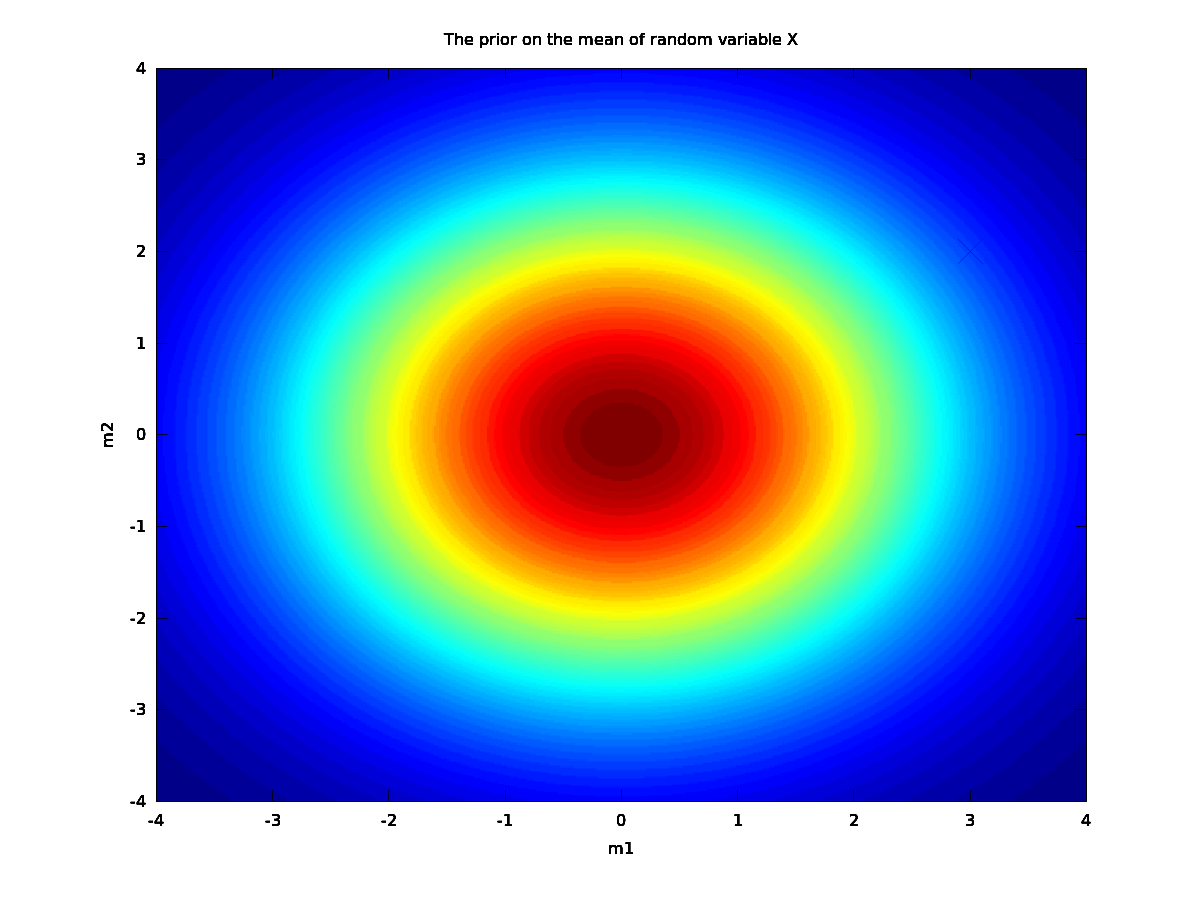
\includegraphics[width=7cm]{prior_of_mean}\\
The prior $p(\mu)$.
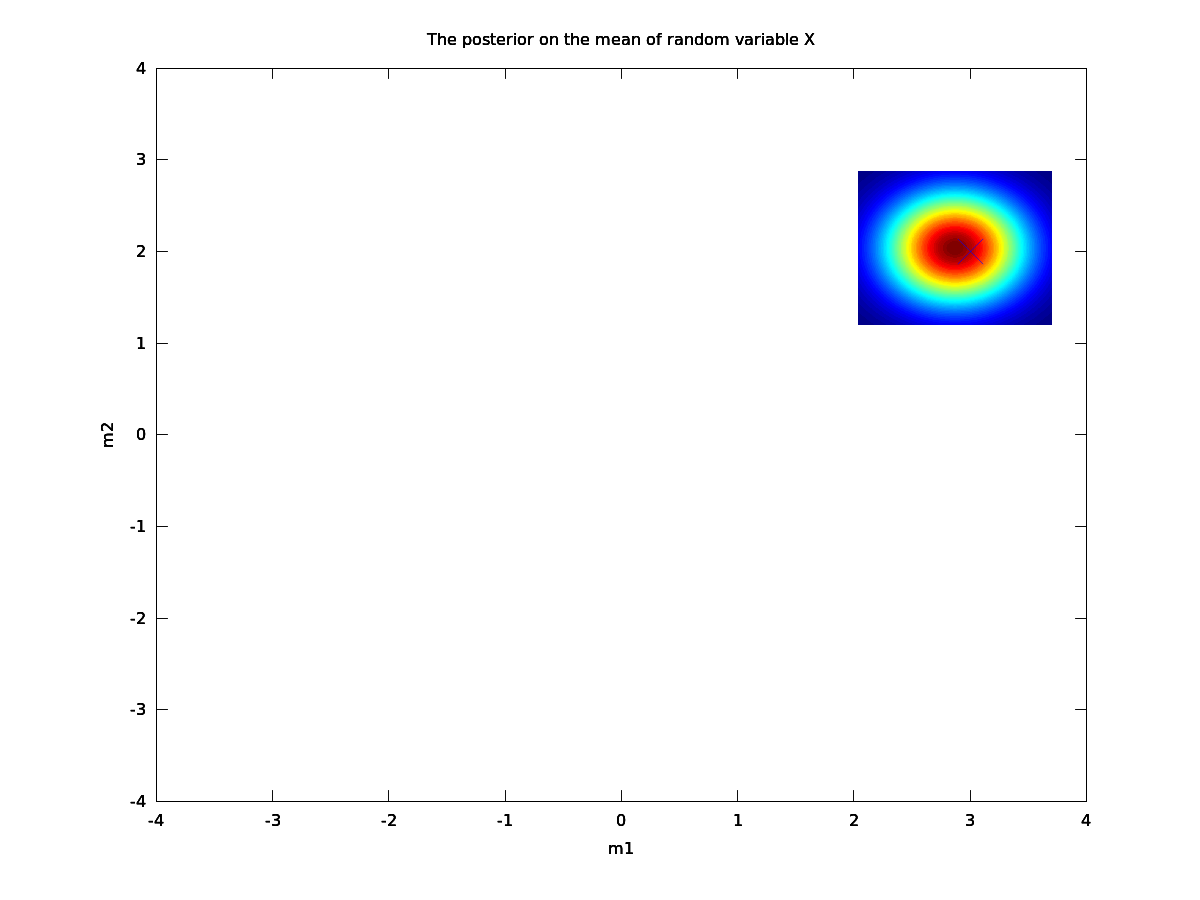
\includegraphics[width=7cm]{posterior_of_mean}\\
The posterior estimate $p(\mu|\mathbf{X}_{1\ldots33})$ (i.e. after
33 observations).
\caption{Bayesian estimation of the mean $\mu$ of RV $\mathbf{x}$ given that
we know the covariance $\Sigma$. The actual position of the mean
is at (3,2) and is marked with a (rather faint) 'X'. The important
point here is not so much that after observing $\mathbf{X}_{1\ldots33}$
the estimate of the mean is pretty close (ML estimation will also
give that), but that the uncertainty about the estimate is also quantified.
Subtly beautiful!}
\label{fig:bayesmeanest2d}
\end{figure}



\subsubsection{Known $\mathbf{\mu}$, unknown $\Sigma$}

\textbf{Dont bother, this does not work.} $\Sigma$ remains uncorrelated
with both $\mathbf{\mu}$ and $\mathbf{X}$, so we can not infer anything
about it. It seems that we will have to bite the bullet and add a
NIW (Normal Inverse Wishart) to EMDW.

Here the linear Gaussian approach will fail us, the model is inherently
non-linear and the conjugate priors no longer are Gaussian (either
gamma or Wishart). However, in the following we will make use of sigma
points to model the result of this non-linear operation once again
with a Gaussian.

Because of symmetry there is $\frac{D(D+1)}{2}$ components we need
to model in $\mathbf{\Sigma}$. It makes sense to model the variances
(on the diagonal) differently from the covariances (off-diagonal)
-- we briefly postpone the discussion of the details of this to the
next paragraph. Assuming that we have a $\frac{D(D+1)}{2}$-dimensional
Gaussian density available for these components, we can proceed to
find its $2\frac{D(D+1)}{2}+1=D^{2}+D+1$ sigma points. Each of these
sigma points represents a different covariance matrix, and this covariance
matrix describes the spread around the known $D$-dimensional mean
vector $\mathbf{\mu}$. Each such combination can thus be represented
by $2D+1$ sigma points giving a total of $(2D+1)(D^{2}+D+1)=2D^{3}+2D^{2}+3D+1$
sigma points, each being a $D$-dimensional sample of $\mathbf{X}$.
Combined with the original $\frac{D(D+1)}{2}$-dimensional $\Sigma$
we therefore have a $\frac{D^{2}+3D}{2}$-dimensional joint $p(\mathbf{X},\Sigma)$.

We now return to the topic of how exactly to model the prior on the
covariances: Because we are modelling a covariance matrix which is
supposed to be positive definite, with a Gaussian which implicitly
has infinite (and thus also negative) support, we are running a severe
risk of running into trouble. Indeed, at this moment I still am unsure
if the procedure I am about to describe is adequate to save our butts,
but lets give it a shot.

It seems that the safest place to start is the correlation coefficient
version of the desired covariance matrix (see \ref{par:corr_coef_form}).
In this normalized version all variances are unity, and the magnitude
of all covariances should be strictly less than one (and even then
we are still not guaranteed that the matrix as a whole is positive
definite).
\begin{itemize}
\item If we now represent these normalised variances $\rho_{ii}$ with Gaussians
with a mean value
\begin{equation}
\mu_{\rho_{ii}}=1,
\end{equation}
 we should try to keep their standard deviations $\sigma_{\rho_{ii}}$small
enough to make negative values of $\rho_{ii}$ very unlikely. Since
samples exceeding about three standard deviations away from the mean
should be rare, this seems to imply that we should choose these standard
deviations at about $\sigma_{\rho_{ii}}=\frac{1}{4}$. But we should
also remember that we are going to represent them via sigma points
which, at least in the standard version we use here, are placed at
about $\sqrt{D+0.5}$ standard deviations away from the mean and this
also should still be positive. Therefore we have
\begin{equation}
\sigma_{\rho_{ii}}\leq\text{min}(\frac{1}{4},\frac{1}{\sqrt{D+0.5}}).
\end{equation}

\item For the off-diagonal correlation coefficients we know that $-1<\rho_{ij}<1$.
Therefore a mean
\begin{equation}
\mu_{\rho_{ij}}=0,
\end{equation}
and standard deviations
\begin{equation}
\sigma_{\rho_{ij}}\leq\text{min}(\frac{1}{4},\frac{1}{\sqrt{\frac{D(D-1)}{2}+0.5}})
\end{equation}
 seems appropriate.
\item As a final step we now need to rescale to the actual non-normalised
variances we want to use. For the normalised version we currently
have:
\[
\mathbf{\rho}\sim\mathcal{N}\left(\left[\begin{array}{c}
\mathbf{1}_{D}\\
\mathbf{0}_{\frac{D(D-1)}{2}}
\end{array}\right],\left[\begin{array}{cc}
\sigma_{\rho_{ii}}^{2}I_{D} & \mathbf{0}\\
\mathbf{0} & \sigma_{\rho_{ij}}^{2}I_{\frac{D(D-1)}{2}}
\end{array}\right]\right).
\]
Assuming that we actually wanted variances $\sigma_{i}^{2}$ as the
expected value of the diagonal elements of $\mathbf{X}$'s covariance
matrix $\Sigma,$ we simply rescale to $\mathbf{\gamma}_{ii}=\sigma_{i}^{2}\mathbf{\rho}_{ii}$
to get:
\begin{equation}
\mathbf{\gamma}\sim\mathcal{N}\left(\left[\begin{array}{c}
\sigma_{1}^{2}\\
\vdots\\
\sigma_{D}^{2}\\
0_{1}\\
\vdots\\
0_{\frac{D(D-1)}{2}}
\end{array}\right],\left[\begin{array}{cccccc}
\sigma_{1}^{4}\sigma_{\rho_{ii}}^{2} & 0 & \hdots & \hdots & \hdots & 0\\
0 & \ddots & \ddots & \ddots & \ddots & \vdots\\
\vdots & \ddots & \sigma_{D}^{4}\sigma_{\rho_{ii}}^{2} & \ddots & \ddots & \vdots\\
\vdots & \ddots & \ddots & \sigma_{1}^{2}\sigma_{2}^{2}\sigma_{\rho_{ij}}^{2} & \ddots & \vdots\\
\vdots & \ddots & \ddots & \ddots & \ddots & 0\\
0 & \hdots & \hdots & \hdots & 0 & \sigma_{(D-1)}^{2}\sigma_{D}^{2}\sigma_{\rho_{ij}}^{2}
\end{array}\right]\right).
\end{equation}



For the istropic case we, of course, simply replace $\sigma_{i}^{2}=\sigma^{2}$.

\end{itemize}

\subsubsection{Both $\mathbf{\mu}$ and $\Sigma$ unknown}

\textbf{Dont bother, this does not work.} $\Sigma$ remains uncorrelated
with both $\mathbf{\mu}$ and $\mathbf{X}$, so we can not infer anything
about it. It seems that we will have to bite the bullet and add a
NIW (Normal Inverse Wishart) to EMDW.

Now things are doubly non-linear -- firstly due to $\Sigma$ being
quadratic, and secondly because we are combining two different sets
of random variables ($\mathbf{\mu}$ and $\Sigma$) into the estimate
densities in the estimate of a third ($\mathbf{X}$). Only do this
if you have non-trivial estimates available for both $\mathbf{\mu}$
and $\Sigma$, otherwise you are very likely to end up with a diagonal
covariance matrix for the final joint, making everything independent.
Not very helpful.

We use the same machinery we implemented for the known $\mathbf{\mu}$,
unknown $\Sigma$ case, but now repeated for each of the $2D+1$ sigma
points of $\mathbf{\mu}$. This gives us an impressive grand total
of $(2D+1)(2D^{3}+2D^{2}+3D+1)$ sigma points and the dimension of
the joint $p(\mathbf{X},\mathbf{\mu},\Sigma)$ is $\frac{D^{2}+5D}{2}$.


\chapter{The Mixture Gaussian (MG) distribution}

\section{Purpose:}
\section{Operators}

\begin{tabular}{lllll}
  Parameterisation         & Operator             & Result                   & Details & Notes\\ \hline
                           & Product              &                          &         & \parbox{0.3\textwidth}{}\\
                           & Divide               &                          &         & \parbox{0.3\textwidth}{}\\
                           & Sum-marginalise      &                          &         & \parbox{0.3\textwidth}{Integrate over subset}\\
                           & Max-marginalise      &                          &         & \parbox{0.3\textwidth}{Observe subset at mode}\\
                           & Observe/reduce       &                          &         & \parbox{0.3\textwidth}{}\\
                           & Normalise            &                          &         & \parbox{0.3\textwidth}{}\\
                           & Dampen               &                          &         & \parbox{0.3\textwidth}{}\\
                           & Distance             &                          &         & \parbox{0.3\textwidth}{}\\
                           & Sample               &                          &         & \parbox{0.3\textwidth}{}\\
\end{tabular}

\chapter{The Conditional Gaussian (CG) distribution} \label{sec:CG}

\section{Purpose}
Let's consider the case where we have a particular discrete RV $D$
dictating which continuous Gaussian applies to a continuous random
vector $X$. (For instance used in a Gaussian classifier where $D$
indicates the class.) We show this as $p(X|D)$. If we now multiply
with $p(D)$ we get the joint $p(X,D)= p(X|D)p(D)$. This looks very
much like a Mixture Gaussian, but with the mixture weights dependent
on the distribution of $D$.  Marginalising $D$ out of this leaves us
with $X$ described by an explicitly mixture Gaussian (i.e. with fixed
weights).  (Carefully note how a CG and an MG differs.)

Now consider the product $p(X|D)p(X)$, something that frequently occur
in a message passing scheme. In general $p(X)$ will match $p(X|D)$
better for certain values of $D$ than for others. Those cases should
result in the product being ``higher'' around the centroid than what
it would be for cases where the two distributions are very different.
This relative scaling will reflect in a non-normalised $g$ value of
the canonical form. I.e. with CGs (and other extensions of it such as
CLGs), we have to explicitly maintain the $g$ value of the canonical
form.

\section{Ramifications:}
Can we only send out a message after having received an incoming
$p(D)$? If so this will have message ordering implications.  Or would
it be possible to send some sort of vacuous message at such a
premature request?

\section{Operators}
\begin{tabular}{lllll}
  Parameterisation         & Operator             & Result                   & Details & Notes\\ \hline
                           & Product              &                          &         & \parbox{0.3\textwidth}{}\\
                           & Divide               &                          &         & \parbox{0.3\textwidth}{}\\
                           & Sum-marginalise      &                          &         & \parbox{0.3\textwidth}{Integrate over subset}\\
                           & Max-marginalise      &                          &         & \parbox{0.3\textwidth}{Observe subset at mode}\\
                           & Observe/reduce       &                          &         & \parbox{0.3\textwidth}{}\\
                           & Normalise            &                          &         & \parbox{0.3\textwidth}{Note, $g$ matters now}\\
                           & Dampen               &                          &         & \parbox{0.3\textwidth}{}\\
                           & Distance             &                          &         & \parbox{0.3\textwidth}{}\\
                           & Sample               &                          &         & \parbox{0.3\textwidth}{}\\
\end{tabular}

\chapter{The Conditional Linear Gaussian (CLG) distribution}

\section{Purpose}
Now we have both a discrete and a continuous conditioning part
$p(Y|X,D)$. I.e. for each different assignment to $D$ we have a
different LG.  For instance, consider a tracking problem where $D$
indicates to which particular state $X_j^{(t)}$ an observation $Y$
should be attributed.

\section{Operators}
\begin{tabular}{lllll}
  Parameterisation         & Operator             & Result                   & Details & Notes\\ \hline
                           & Product              &                          &         & \parbox{0.4\textwidth}{}\\
                           & Divide               &                          &         & \parbox{0.4\textwidth}{}\\
                           & Sum-marginalise      &                          &         & \parbox{0.4\textwidth}{Integrate over subset}\\
                           & Max-marginalise      &                          &         & \parbox{0.4\textwidth}{Observe subset at mode}\\
                           & Observe/reduce       &                          &         & \parbox{0.4\textwidth}{}\\
                           & Normalise            &                          &         & \parbox{0.4\textwidth}{Note, $g$ matters now}\\
                           & Dampen               &                          &         & \parbox{0.4\textwidth}{}\\
                           & Distance             &                          &         & \parbox{0.4\textwidth}{}\\
                           & Sample               &                          &         & \parbox{0.4\textwidth}{}\\
\end{tabular}

\chapter{The Conditional Mixture Gaussian (CMG) distribution}

\section{Purpose:}
\section{Operators}

\begin{tabular}{lllll}
  Parameterisation         & Operator             & Result                   & Details & Notes\\ \hline
                           & Product              &                          &         & \parbox{0.4\textwidth}{}\\
                           & Divide               &                          &         & \parbox{0.4\textwidth}{}\\
                           & Sum-marginalise      &                          &         & \parbox{0.4\textwidth}{Integrate over subset}\\
                           & Max-marginalise      &                          &         & \parbox{0.4\textwidth}{Observe subset at mode}\\
                           & Observe/reduce       &                          &         & \parbox{0.4\textwidth}{}\\
                           & Normalise            &                          &         & \parbox{0.4\textwidth}{Note, $g$ matters now}\\
                           & Dampen               &                          &         & \parbox{0.4\textwidth}{}\\
                           & Distance             &                          &         & \parbox{0.4\textwidth}{}\\
                           & Sample               &                          &         & \parbox{0.4\textwidth}{}\\
\end{tabular}



\chapter{Others}

\begin{itemize}
\item \texttt{Dirichlet<AssignType>}: A Dirichlet prior for categorical
  variables. Unit tests in \texttt{dirichlet.test.cc}.
\item \texttt{Polya<AssignType>}: The combination of a single
  \texttt{Categorical} dependent on a \texttt{Dirichlet} prior, draws
  strongly on the 'Polya' distribution.
\item \texttt{GaussCanonical} (various versions), also with facilities
  for handling Linear Gaussians and Sigma Point Gaussians.  (The Gaussian
  classes are probably in for a major revamp.)
\end{itemize}

\section{Planned}
\begin{itemize}
\item BVG
\item Conditional Gaussian
\item Mixture Gaussian
\item GaussWishart
\end{itemize}

\part{Logarithmic format (planned)}

The above can also be implemented in log format, and I strongly suspect
we want to do that. Log-linear models etc. Probably mostly rely on
different factor operations.

\part{Inference}
\chapter{Basics of message passing}

\section{Loopy message passing}

Figure~\ref{fig:msgpassing} describes one branch of a loopy cluster
graph. It serves as a basic configuration for describing the various
message passing algorithms. For ease of explanation we assume discrete
random variables (i.e. factor marginalisation is done via summation),
but all results also hold for continuous random variables (where
marginalisation is done via integration).

$\Phi_a$ and $\Phi_b$ are the internal factor functions of nodes $a$
and $b$ respectively. (When more than one factor function are
allocated to a cluster, it is their product). As such it is a function
of the random variables involved in those functions, we suppressed
explicit mention of this.

$S_{a,b}$ is the sepset linking nodes $a$ and $b$, i.e. the set of all
variables that those two clusters will exchange information about. It
does so by passing message $\mu_{a,b}$ from node $a$ to $b$ and vice
versa for $\mu_{b,a}$.  We use the notation $\backslash a$ to indicate
the set of all nodes excluding $a$ (i.e. its
complement). Correspondingly:
\begin{align}
  \mu_{\backslash b,a} = \prod_{i \in \backslash b} \mu_{i,a} \nonumber
\end{align}
is the product of all messages entering node $a$, except for the
message $\mu_{b,a}$.

The product of all incoming messages with the cluster internal factors
forms the \emph{cluster belief}:
\begin{align}
  \Psi_a &= \Phi_a \mu_{b,a} \mu_{\backslash b,a} \label{eq:clusterbelief}
\end{align}
for cluster $a$. Similarly the \emph{sepset
  belief} is formed by the product of the two opposing messages
passing through the sepset:
\begin{align}
  \psi_{a,b} &= \mu_{a,b}\mu_{b,a} \label{eq:sepsetbelief}
\end{align}
for sepset $S_{a,b}$.

\begin{figure}[b]
  \begin{centering}
    \psfragfig*[width=0.75\textwidth,crop=pdfcrop,angle=0]{msgpassing}\\
    \caption{Configuration used for explaining message passing
      algorithms. See the text for definitions etc..\label{fig:msgpassing} }
  \end{centering}
\end{figure}
\FloatBarrier

\subsection{Loopy belief \emph{propagation} (a.k.a. the Shafer-Shenoy algorithm)}
This is the most basic belief propagation algorithm upon which the
others build. The details are in Algorithm~\ref{alg:LBP}.

\begin{algorithm}[h]
  \caption{Loopy belief propagation (LBP)}  \label{alg:LBP}
  \begin{description}
  \item[Initialization:] ~\\Form initial messages $\mu_{a,b}$ from all
    source clusters $a$ to their respective destination clusters
    $b$. The standard way to do this is to use vacuous /
    non-informative messages $\mu_{a,b}=1$.  Instead we prefer to
    marginalize each neighbouring cluster to only retain the variables
    specified in the sepset connecting the two clusters i.e.
    \begin{align}
      \mu_{a,b} &= \sum_{\backslash S_{a,b}} \Phi_a. \label{eq:msginit}
    \end{align}
    With a tree structure for our graph these two initializations
    would have turned out to be equivalent. However, in a loopy system
    the order of message passing is important. Our preferred
    initialization allows us to measure how far a message deviates
    from its vacuous version -- using this we can schedule messages in
    order of importance.
  \item[Iteration:]~\\[-2ex]
    \begin{enumerate}
    \item From each source node $a$ to each destination node $b$
      connected to it, take the product of all other messages incoming
      to $a$, (i.e. except $\mu_{b,a}$) with the internal cluster
      factor and then marginalise to only retain the variables
      specified in the sepset $S_{a,b}$:
      \begin{align}
        \mu^{'}_{a,b} &= \sum_{\backslash S_{a,b}} \mu_{\backslash b,a}\Phi_a. \label{eq:msgupdate}
      \end{align}
    \item Monitor convergence by checking the distance
      $d(\mu_{a,b},\mu^{'}_{a,b})$ between the old and new messages. The
      KL-divergence is a good choice for distance. If a message
      converged to within a set margin, its destination cluster needs
      not be propagated further.
    \item $\mu_{a,b} = \mu^{'}_{a,b}.$
    \end{enumerate}
  \item[Termination:]~\\ The above iterations continue until either all
    messages have converged, or a maximum number of iterations were
    completed.
  \end{description}
\end{algorithm}
\FloatBarrier

\subsection{From belief \emph{propagation} to belief \emph{update} (LBU2)}
The trick here is to notice that:
\begin{align}
  \mu^{'}_{a,b} &= \sum_{\backslash S_{a,b}} \mu_{\backslash b,a}\Phi_a \nonumber \\
  &= \sum_{\backslash S_{a,b}} \mu_{\backslash b,a}\Phi_a \mu_{b,a}/\mu_{b,a} \nonumber \\
  &= \left(\sum_{\backslash S_{a,b}} \Psi_a\right)/\mu_{b,a}
  && \text{(from Eq.~\ref{eq:clusterbelief} and using $\backslash S_{a,b}\cap S_{a,b} = \emptyset$)}.  \nonumber
\end{align}
Note in the last step that, since $\mu_{b,a}$ shares no variables with
$\S_{a,b}$, we are free to take it out of the summation. In
Algorithm~\ref{alg:LBU2} we use this to express our message passing
i.t.o. cluster beliefs. It holds some benefits:

\begin{itemize}
\item Graphs with high connectivity can become considerably faster.
\item The full cluster belief can be much more informative. For
  instance, in a discrete model some variable settings can turn out to
  be impossible. Or in a continuous setting where the marginalization
  needs to be approximated, the full cluster belief can focus that
  approximation to the most relevant variable values. This enhances
  convergence of the system.
\end{itemize}

\begin{algorithm}[!h]
  \caption{Basic loopy belief update -- (LBU2)}  \label{alg:LBU2}
  \begin{description}
  \item[Initialization:]~\\[-5mm]
    \begin{enumerate}
    \item Form initial messages as in Algorithm~\ref{alg:LBP}.
    \item In addition each cluster $a$ now forms an initial cluster
      belief $\Psi_a$ as the product of its internal factor(s) with
      all its incoming messages.
    \end{enumerate}
  \item[Iteration:]~\\[-5mm]
    \begin{enumerate}
    \item To send a message from cluster $a$ to cluster $b$, we
      marginalise all variables not contained in the sepset between
      them out, and then we divide by the earlier message from the
      opposite direction, i.e.
      \begin{align}
        \mu^{'}_{a,b} = \left(\sum_{\backslash S_{a,b}} \Psi_a\right)/\mu_{b,a}. \nonumber
      \end{align}
    \item At the destination cluster we need to first remove the
      earlier (previous iteration) version of this message by
      dividing it out. Then the destination cluster gets updated
      by multiplication with the new message, i.e.
      \begin{align}
        \Psi^{'}_{b} = \Psi_b\left(\mu^{'}_{a,b}/\mu_{a,b}\right). \label{eq:clusterupdate}
      \end{align}
    \item Monitor convergence by checking the distance
      $d(\mu_{a,b},\mu^{'}_{a,b})$ between the old and new messages. The
      KL-divergence is a good choice for distance. If a message
      converged to within a set margin, its destination cluster needs
      not be propagated further.
    \item $\mu_{a,b} = \mu^{'}_{a,b}.$
    \end{enumerate}
  \item[Termination:] Same as in Algorithm~\ref{alg:LBP}.
  \end{description}
\end{algorithm}

On the downside, two divisions are required for each message being
passed. And in some cases those divisions can also introduce numerical
sensitivity.

\FloatBarrier
\subsection{Loopy belief \emph{update} (a.k.a. the Lauritzen Spiegelhalter algorithm)}

Now consider the following situation: Initial messages are created as
in Eq~\ref{eq:msginit}, after which the initial cluster and sepset
beliefs are determined from Eqs.~\ref{eq:clusterbelief} and
~\ref{eq:sepsetbelief}. We now want to update the sepset belief to also
reflect the information in messages $\mu_{\backslash b,a}$. From
definition we know this to be:
\begin{align}
  \psi^{'}_{a,b}
  &= \mu^{'}_{a,b}\mu_{b,a} \nonumber \\
  &= \left(\sum_{\backslash S_{a,b}} \mu_{\backslash b,a}\Phi_a\right)\mu_{b,a} && \text{(from Eq.~\ref{eq:msgupdate})} \nonumber\\
  &= \sum_{\backslash S_{a,b}} \Psi_a, && \text{(from Eq.~\ref{eq:clusterbelief})} \label{eq:sepsetupdate}
\end{align}
i.e. marginalising the cluster belief directly gives us the updated sepset belief! Now consider:
\begin{align}
  \Psi_b\frac{\psi^{'}_{a,b}}{\psi_{a,b}}
  &= \Psi_b \frac{\mu^{'}_{a,b}\mu_{b,a}}{\mu_{a,b}\mu_{b,a}} \nonumber \\
  &= \Psi^{'}_b, && \text{(from Eq.~\ref{eq:clusterupdate})}
\end{align}
i.e. we can update a cluster belief by dividing the old sepset belief
out and multiplying the new one in. Note that in contrast to
Algorithm~\ref{alg:LBU2} we now only do one factor division.
\begin{algorithm}[!h]
  \caption{Loopy belief update -- (LBU)}  \label{alg:LBU}
  \begin{description}
  \item[Initialization:]~\\[-5mm]
    \begin{enumerate}
    \item Form initial messages as in Algorithm~\ref{alg:LBP}.
    \item Form cluster beliefs as in Algorithm~\ref{alg:LBU2}.
    \item Furthermore, each sepset $S_{a,b}$ now forms an initial
      sepset belief $\psi_{a,b}$ as the product of the two opposing
      messages passing through it.
    \end{enumerate}
  \item[Iteration:]~\\[-5mm]
    \begin{enumerate}
    \item To send a message from cluster $a$ to cluster $b$, update the sepset belief:
      \begin{align}
        \psi^{'}_{a,b}
        &= \sum_{\backslash S_{a,b}} \Psi_a. \nonumber
      \end{align}
    \item Use this updated sepset belief to update the target cluster belief:
      \begin{align}
        \Psi^{'}_b & = \Psi_b\frac{\psi^{'}_{a,b}}{\psi_{a,b}} \nonumber
      \end{align}
    \item Monitor convergence by checking the distance
      $d(\psi_{a,b},\psi^{'}_{a,b})$ between the old and new sepset beliefs. The
      KL-divergence is a good choice for distance. If it
      converged to within a set margin, its destination cluster needs
      not be propagated further.
    \item $\psi_{a,b} = \psi^{'}_{a,b}.$
    \end{enumerate}
  \item[Termination:] The above iterations continue until either all
    sepset beliefs have converged, or a maximum number of iterations
    were completed.
  \end{description}
\end{algorithm}

\FloatBarrier
\section{Residual error propagation}

To start off, inference is done over some graph of probabilistic
factors. In our case we use an LTRIP clustergraph (see
\texttt{clustergraph.hpp} for details) -- the procedure for configuring
it is nicely explained in \cite{Streicher2017}.

The inference code is contained in \texttt{lbu\_cg.\{hpp,cc\}}. For a
nitty-gritty level of understanding one must be aware of the important
datastructures and their use. The \texttt{loopyBU\_CG} inference
procedure primarily relies on the following three parameters:
\begin{itemize}
\item \texttt{std::vector< rcptr<Factor> > ClusterGraph::factorPtrs}:
  These are the \texttt{Factor}s that the inference is going to
  operate on. See \texttt{clustergraph.hpp} for more detail.
\item \texttt{std::map< Idx2, rcptr<Factor> > ssBeliefs}: This
  contains the marginal beliefs over the sepsets at any given stage of
  computation. The \texttt{Idx2} field is a
  \texttt{std::pair<unsigned,unsigned>} indicating between which two
  factors this sepset resides.
\item \texttt{MessageQueue msgQueue} is a type of priority queue of
  which the important elements are a \texttt{Idx2} recording from
  which factor to which the message is passed, as well as a priority
  value indicating how important this message is. Only priorities
  exceeding a threshold are added to this queue. When it is empty the
  inference is considered converged. (See \texttt{messagequeue.hpp}
  for more detail.) Typically, but not necessarily so, this is empty
  on entry and exit. If not empty on entry it will be taken to contain
  the initial state for messages to be passed. If not empty on exit it
  indicates that the inference procedure was prematurely terminated
  (and can be continued from that state).

\end{itemize}

For explaining a typical inference iteration, let us assume that
\texttt{ssBeliefs} already contains the marginal sepset beliefs
(messages) between factors, \texttt{factorPtrs} already contains the
marginal cluster beliefs (the effect of the current sepset beliefs are
already absorbed in this). The head of \texttt{msgQueue} tells us
which one of those messages currently has the highest priority. From
this we then also know from which factor to which this sepset belief
was passed. At this point the source factor, its destination factor
and the sepset between them is already updated. What now needs to be
done is to update the factors beyond the destination factor as well as
the sepsets between them and our current destination factor.
\begin{itemize}
\item Pop the head of \texttt{msgQueue}. We now use its destination
  index as the new ``source'' factor index for this iteration, and
  all the factors it connects to (excluding our original source
  factor) its destination factors. For each of these destination
  factors:
  \begin{itemize}
  \item Marginalize the source factor to the scope of the sepset
    between the source and destination factors. This becomes the new
    sepset belief. Find the distance between it and the previous
    sepset belief. If this difference exceeds a threshold, record
    this message in the \texttt{msgQueue}.
  \item Divide this new sepset belief by the old sepset belief and
    absorb the result in the destination factor.
  \end{itemize}

\end{itemize}


\section{Continuing after interrupting and modifying the inference procedure}
If the inference is temporarily interrupted, one or more of the
\texttt{std::vector< rcptr<Factor> > ClusterGraph::factorPtrs} can
modified externally before continuing with inference. To do so, use
such modified factors as new source factors and complete one iteration
of message updating as described above. After applying these changes a
call \texttt{loopyBU\_CG} will proceed with the inference procedure.

\pagebreak

\section*{Contributors}
The following people contributed towards developing this
document:\\ ...


\bibliographystyle{ieeetr}
\bibliography{pgm}

\end{document}
